\chapter{Projective Planes}

\section{Incidence Geometry}

In this chapter we follow the exposition of \citep{kiss2019finite}.

\begin{defn}
    An \textsl{incidence geometry} is a triple $\igeo$, where $\pts$ and $\blocks$ are nonempty disjoint sets and $\incidence$ is a subset of $\pts\times\blocks$.
    
    The elements of $\pts$ are called \textsl{points} and are usually denoted with capital letters $A$, $B$, $C$, etc. The elements of $\blocks$ are \textsl{blocks}. They are denoted with lower-case letters such as $\block a$, $\block b$, $\ell$, etc. Finally, $\incidence$ is the \textsl{incidence relation}, and expressions like ``$P$ and $\block b$ are incident'', etc. will mean $P\incidence\block b$.
\end{defn}

\begin{xmpls}${}$
    \begin{enumerate}[a),font=\upshape]
        \item \textbf{Steiner System.} Define the incidence geometry where $\pts=\set{1,2,3,4,5}$, $\blocks$ is the set of parts of $\pts$ having $3$ elements, and $\incidence$ is the membership relation.
        $$
            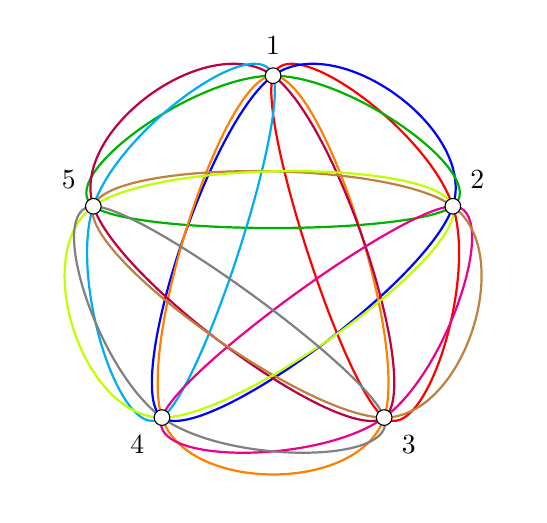
\begin{tikzpicture}[
                point/.style={draw, circle, fill=white, inner sep=2pt, minimum size=5pt},
                curve/.style={thick, tension=0.8}, % Style for the block curves
                scale=0.8
              ]
            
              \def\radius{3cm} % Radius for placing points
            
              % Define Coordinates for the 5 points as vertices of a pentagon
              \coordinate (P1) at (90:\radius);
              \coordinate (P2) at (18:\radius);
              \coordinate (P3) at (-54:\radius); % 306 degrees
              \coordinate (P4) at (-126:\radius); % 234 degrees
              \coordinate (P5) at (162:\radius);
            
              % Define a list of colors for the 10 blocks
              \colorlet{c1}{red}
              \colorlet{c2}{blue}
              \colorlet{c3}{green!70!black}
              \colorlet{c4}{orange}
              \colorlet{c5}{purple}
              \colorlet{c6}{cyan}
              \colorlet{c7}{magenta}
              \colorlet{c8}{brown}
              \colorlet{c9}{lime}
              \colorlet{c10}{gray}
            
              % --- Draw the 10 Blocks (Curves) ---
              % Draw these first so points appear on top.
              % Each command draws a smooth closed curve through 3 specified points.
            
              \draw[curve, c1] plot[smooth cycle] coordinates {(P1) (P2) (P3)}; % Block {1,2,3}
              \draw[curve, c2] plot[smooth cycle] coordinates {(P1) (P2) (P4)}; % Block {1,2,4}
              \draw[curve, c3] plot[smooth cycle] coordinates {(P1) (P2) (P5)}; % Block {1,2,5}
              \draw[curve, c4] plot[smooth cycle] coordinates {(P1) (P3) (P4)}; % Block {1,3,4}
              \draw[curve, c5] plot[smooth cycle] coordinates {(P1) (P3) (P5)}; % Block {1,3,5}
              \draw[curve, c6] plot[smooth cycle] coordinates {(P1) (P4) (P5)}; % Block {1,4,5}
              \draw[curve, c7] plot[smooth cycle] coordinates {(P2) (P3) (P4)}; % Block {2,3,4}
              \draw[curve, c8] plot[smooth cycle] coordinates {(P2) (P3) (P5)}; % Block {2,3,5}
              \draw[curve, c9] plot[smooth cycle] coordinates {(P2) (P4) (P5)}; % Block {2,4,5}
              \draw[curve, c10] plot[smooth cycle] coordinates {(P3) (P4) (P5)}; % Block {3,4,5}
            
              % --- Draw the 5 Points ---
              % Draw points on top of the curves, with labels slightly outside.
              \foreach \i/\pos in {1/above, 2/above right, 3/below right, 4/below left, 5/above left} {
                \node[point, label={[label distance=1pt]\pos:$\i$}] at (P\i) {};
              }
              % Alternatively, place labels inside slightly larger nodes:
              % \foreach \i in {1,...,5} {
              %   \node[draw, circle, fill=white, inner sep=0pt, minimum size=12pt] at (P\i) {\i};
              % }
            \end{tikzpicture}
        $$
        This incidence geometry is known as the Steiner System $S(3,3,5)$.

        \item \textbf{Affine Plane of Order 2.} Here $\pts=\set{1,2,3,4}$, $\blocks$ is the set of parts with $2$ elements and $\incidence$ is the membership relation.
        $$
            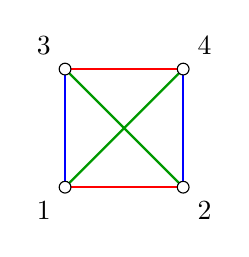
\begin{tikzpicture}[
                scale=1.5, % Adjust scale as needed
                point/.style={draw, circle, fill=white, inner sep=1.5pt, minimum size=4pt}, % Style for points
                line/.style={thick} % Style for lines
              ]
            
              % Define Coordinates for the 4 points (corners of a square)
              \coordinate (P1) at (0,0);   % Point 1 (bottom-left)
              \coordinate (P2) at (1,0);   % Point 2 (bottom-right)
              \coordinate (P3) at (0,1);   % Point 3 (top-left)
              \coordinate (P4) at (1,1);   % Point 4 (top-right)
            
              % --- Draw the 6 Lines (Blocks) ---
              % Grouped and colored by parallel class for clarity
            
              % Parallel Class 1 (Horizontal lines: {1,2} and {3,4})
              \draw[line, red] (P1) -- (P2);
              \draw[line, red] (P3) -- (P4);
            
              % Parallel Class 2 (Vertical lines: {1,3} and {2,4})
              \draw[line, blue] (P1) -- (P3);
              \draw[line, blue] (P2) -- (P4);
            
              % Parallel Class 3 (Diagonal lines: {1,4} and {2,3})
              \draw[line, green!60!black] (P1) -- (P4);
              \draw[line, green!60!black] (P2) -- (P3);
            
              % --- Draw the 4 Points ---
              % Draw points last so they are on top of the lines
              % Labels are placed relative to the point position
              \node[point, label=below left:$1$] at (P1) {};
              \node[point, label=below right:$2$] at (P2) {};
              \node[point, label=above left:$3$] at (P3) {};
              \node[point, label=above right:$4$] at (P4) {};
            
            \end{tikzpicture}
        $$
        This incidence geometry, denoted $\AG(2,2)$, satisfies the following properties:
        \begin{enumerate}[1.]
            \item Every pair of different points defines one, and only one, line (element of $\blocks$).
            \item If the point $P$ is not in the block $\block b$, then there is a unique block $\ell$ such that $P\in\ell$ and $\ell\cap\block b=\emptyset$.
            \item Every block contains (exactly) $2$ points.
            \item Every point belongs to (exactly) $3$ blocks.
        \end{enumerate}
    \end{enumerate}
\end{xmpls}

\begin{ntn}
    Given an incidence geometry\/ $\Gamma=\igeo$ its \textsl{dual} is defined as\/ $\Gamma^*=(\blocks,\pts,\incidence^{-1})$. Clearly, $\Gamma^*$ is an incidence geometry and\/ $\Gamma^{**}=\Gamma$.
\end{ntn}

\begin{ntn}\label{ntn:pts-bks}
    Given a block\/ $\block b$ in an incidence geometry\/ $\igeo$, the \textsl{trace} of\/ $\block b$ is the set\/ $\tr(\block b)$ of points incident with\/ $\block b$. Dually, given a point\/ $A$, the \textsl{pencil} of\/ $A$ is the set\/ $\pl(A)$ of blocks incident with\/ $A$.
\end{ntn}

\section{Projective Plane}

\begin{defns}${}$\label{defn:incidence-geometry}

    Given an incidence geometry $\Gamma=\igeo$,
    \begin{enumerate}[a),font=\upshape]
        \item a set of points is 
            \begin{itemize}
                \item \textsl{collinear} when all its elements are incident with the same block,
                
                \item in \textsl{general position} if no three of them are collinear,

                \item a \textsl{quad} if it consists of $4$ points in general position;
            \end{itemize}

            \item a set of lines is \textsl{concurrent} when there is a point incident with all its elements;
            
            \item a \textsl{triangle} is a non-collinear set of $3$ points;

            \item a \textsl{morphism} from $\Gamma$ to another incidence geometry $\igeo[']$ is a pair $(f,\varphi)$ where $f\colon\pts\to\pts'$ and $\varphi\colon\blocks\to\blocks'$ are maps that satisfy
            $$
                A\incidence\ell\implies 
                    f(A)\incidence'\varphi(\ell)
            $$
            for $A\in\pts$ and $\ell\in\blocks$;

            \item an \textsl{incidence subgeometry} of $\Gamma$ is a triple $\igeo[']$ where $\pts'\subseteq{\pts}$, $\blocks'\subseteq{\blocks}$ and $\incidence'$ is \textsl{induced} by~$\incidence$, i.e., ${\incidence'}={(\pts'\times\blocks')}\cap{\incidence}$.
    \end{enumerate}
    
\end{defns}

\begin{defn}
    An incidence geometry $\igeo$ is a \textsl{projective plane} if it satisfies:
    \begin{enumerate}[
        p$_{\arabic*}$,
        ref=\textsc{p$_\arabic*$},
        font=\scshape]
        \item \label{P1}Every pair of distinct points of $\pts$ is incident with one, and only one, block in~$\blocks$.
        
        \item \label{P2}For every pair of distinct blocks in $\blocks$ there exists one, and only one, point in $\pts$ incident with them.

        \item \label{P3}For every block in $\blocks$ there are at least $3$ distinct points in~$\pts$ incident with the block.

        \item \label{P4}Every point in $\pts$ is incident with, at least, $3$ distinct blocks in~$\blocks$.
    \end{enumerate}
\end{defn}

%\newcommand{\PP}[1]{{\upshape{\textsc{\ref{P#1}}}}}
\newcommand{\PP}[1]{{\upshape\ref{P#1}}}

\begin{rem}
    The dual of a projective plane is a projective plane.
\end{rem}

\begin{ntn}
    Blocks in a projective plane are called \textsl{lines}. Axioms\/ \PP1 and\/ \PP2 allow us to introduce the notation\/ $AB$ to refer to the line incident with the points\/ $A$ and\/ $B$ whenever\/ $A\ne B$. Similarly, given two lines\/ $\block b\ne\block c$ the point incident with both of them will be denoted\/ $\block b\wedge\block c$.
\end{ntn}

\begin{rem}\label{rem:rotation-rule} [Rotation Rule]
    A trivial but useful observation is that if $A$, $B$ and $C$ are distinct, then
    \begin{align}
        A\incidence BC \iff C&\incidence AB \iff B\incidence CA,
        \label{eq:rotation-rule}
    \end{align}
    We will refer to these equivalences as the \textsl{rotation rule}.
\end{rem}

\begin{rem}\label{rem:quad-rule} [Quad Rule]
    From a set of four points $\set{A,B,C,D}$ we can form $\binom{4}{3}=4$ distinct triads, namely
    \[
    \begin{array}{cccc}
        A & B & C & D\\
        \hline
        \textcolor{red}{\mbf\cdot} & \textcolor{red}{\mbf\cdot} & \mbf\cdot \\
        \textcolor{red}{\mbf\cdot} & \textcolor{red}{\mbf\cdot} & & \mbf\cdot \\
        \mbf\cdot & & \textcolor{red}{\mbf\cdot} & \textcolor{red}{\mbf\cdot} \\
        & \mbf\cdot & \textcolor{red}{\mbf\cdot} & \textcolor{red}{\mbf\cdot}
    \end{array}
    \]
    Therefore, to show that these four points form a quad, it suffices to check that none of the triads is collinear. For instance, $C,D\nincidence AB$ and $A,B\nincidence CD$.
\end{rem}

\makeatletter
% page 18
\newcommand\apostrophes[1]{\expandafter\@apostrophes\csname c@#1\endcsname}
\newcommand{\@apostrophes}[1]{%
  \ifcase\numexpr#1\relax
    \or '\hphantom' \or '' \or ''' \or '''' \or '''''%
  \else '''''%
  \fi
}
\makeatother
\AddEnumerateCounter*{\apostrophes}{\@apostrophes}{6}


\begin{lem}\label{lem:alternative-projective-axiom}
    An incidence geometry\/ $\igeo$ is a projective plane if, and only if, it satisfies properties\/ \PP1 and\/ \PP2, and one of the following two conditions:
    \begin{enumerate}[font=\scshape]
        \item[p$_3$\!'\hphantom'] There are four points in general position.
        \item[p$_3$\!''] ${\incidence}\ne\emptyset$ and given two lines, there is always a point not incident with either of them.
    \end{enumerate}
\end{lem}

  
\newcommand{\Ptprime}{{\upshape\textsc{\hyperref[lem:alternative-projective-axiom]{p$_3$\!'}}}}

\newcommand{\Ptdprime}{{\upshape\textsc{\hyperref[lem:alternative-projective-axiom]{p$_3$\!''}}}}

\begin{proof}
    Let $\Gamma$ denote the geometry and suppose that $\Gamma$ conforms to axioms~\PP1, \PP2 and \Ptprime. To verify \PP3 take a line $\ell$. Let $A,B,C,D$ be $4$ points in general position. Without loss of generality, we may assume that $A\nincidence\ell$. Using \PP2, define $P_X=XA\wedge\ell$ for $X=B,C,D$. Since $P_X=P_Y$ would imply that $A,X,Y$ are collinear, we see that $P_B,P_C,P_D$ are distinct and incident with~$\ell$. Thus, $\Gamma$ satisfies \PP3.
    
    Note that the dual $\Gamma^*$ satisfies \PP1, and \PP2. To verify \Ptprime\ take four points $A$, $B$, $C$, $D$ in general position in $\Gamma$. Then the lines $AB$, $BC$, $CD$ and $CA$ define four points in general position in~$\Gamma^*$. Otherwise we would have, say, $AB$, $BC$ and $CD$ concur at a point $O$. Since $O=B$ implies $B\incidence CD$, which is impossible, we deduce that $O\ne B$. Then $B\incidence OB$, and the \rr\ implies that $A\incidence OB$, and $C\incidence OB$, in contradiction with our hypothesis. Hence, $\Gamma^*$ satisfies \Ptprime\ and we can apply what we showed before, i.e., that $\Gamma^*$ satisfies \PP3. This means that $\Gamma$ satisfies~\PP4. Hence, $\Gamma$ is a projective plane.

    Now assume that $\Gamma$ is a projective plane. Pick a point $O$. By \PP4 there are two (actually three) distinct lines $\block a,\block b$ incident with $O$. According to \PP3 we can pick two points $A$ and $A'$ incident with $\block a$ and $B$ and $B'$ incident with $\block b$, all of which are pairwise distinct and distinct from~$O$.
    $$
        \begin{tikzpicture}[scale=0.45,
            dot/.style={circle, fill=black, inner sep=1.5pt} % Style for points
          ]
        
          % 1. Pick a point O
          \coordinate (O) at (0,0);
        
          % 2. Take two distinct lines a, b incident with O
          % Define line 'a' (e.g., slope -1/3)
          \coordinate (a_dir) at (3,-2.2); % Direction vector for line a
          \draw ($(O)!-1.5!(a_dir)$) -- ($(O)!1.5!(a_dir)$) node[right] {$\block a$};
        
          % Define line 'b' (distinct from a, e.g., slope 2/1)
          \coordinate (b_dir) at (1,2.5); % Direction vector for line b
          \draw ($(O)!-1.4!(b_dir)$) -- ($(O)!1.5!(b_dir)$) node[left] {$\block b$};
        
          % 3. Pick two points A and A' incident with a, distinct from O and each other
          % Place A along the positive direction of a_dir from O
          \coordinate (A) at ($(O)!1!(a_dir)$);
          % Place A' along the negative direction of a_dir from O
          \coordinate (Aprime) at ($(O)!-1!(a_dir)$);
        
          % 4. Pick two points B and B' incident with b, distinct from O and each other
          % Place B along the positive direction of b_dir from O
          \coordinate (B) at ($(O)!1.1!(b_dir)$);
          % Place B' along the negative direction of b_dir from O
          \coordinate (Bprime) at ($(O)!-1.2!(b_dir)$);
        
          % --- Draw and label the points ---
          % Ensure labels use math mode for primes: $A'$ and $B'$
          \node[dot, label=right:$O$] at (O) {};
          \node[dot, label=below:$A$] at (A) {};
          \node[dot, label=above:$A'$] at (Aprime) {};
          \node[dot, label=right:$B$] at (B) {};
          \node[dot, label=right:$B'$] at (Bprime) {};
        
        \end{tikzpicture}
    $$
    Let's see that $A,A',B,B'$ are in general position. Otherwise, say $A$, $A'$, and $B$ were collinear. Then $O,B\incidence AA'$ and so $OB=AA'$. Since $O\incidence BB'$, by the \rr\ $B'\incidence OB$. Hence, $\block b=BB'=OB=AA'=\block a$, which isn't the case. It follows that $\Gamma$ satisfies~\Ptprime.

    To see that \Ptdprime\ also holds true when $\Gamma$ is a projective plane, take two distinct lines $\block a$ and $\block b$. By \PP3 there are two points $A\incidence\block a$ and $B\incidence\block b$, both distinct from $O=\block a\wedge\block b$. Then, $OA=\block a$ and $OB=\block b$. Furthermore, by the same axiom there is a third point $C$ on $AB$, distinct from $A$ and $B$. Thus, $C$ cannot be incident with $\block a$ because that would imply $C=\block a\wedge\block c=OA\wedge\block c=A$, which is not. Similarly, $C$ cannot be incident with $\block b$, proving \Ptdprime.

    It remains to be seen that \PP1, \PP2 and P3'' imply P3'. According to P3'' we can pick two points $A$ and $B$ and a line $\block a$ with $A\incidence\block a$ and $B\nincidence\block a$. Let $\block b=AB$. Then $\block a\ne\block b$ and there exists $D$ not incident with either $\block a$ or $\block b$. Let $\block c=BD$ and $C=\block a\wedge\block c$. Pick $E$ not incident with either $\block a$ or $\block c$.
    $$
        \begin{tikzpicture}[
                scale=0.7,
                font=\small,
                point/.style={circle, fill, inner sep=1.1pt, draw=black},
                line/.style={thick},
                initial_line/.style={line, black},
                constructed_line/.style={line, orange},
                second_construction/.style={line, green!60!black}
            ]
            
            % --- Define initial elements ---
            % Define line 'a' using a named path for intersections
            \path[name path=aLine] (-1,0) -- (7,0);
            % Define points A on line 'a' and B not on 'a'
            \coordinate (A) at (1,0);
            \coordinate (B) at (2,3);
            
            % --- Draw initial elements ---
            \draw[initial_line] (-1,0) -- (7,0) node[right] {$\block a$};
            \node[point, label={above left:$A$}] at (A) {};
            \node[point, label={right:$B$}] at (B) {};
            
            % --- First set of constructions ---
            % Define and draw line b = AB
            \path[name path=bLine] ($(A)!-0.5cm!(B)$) -- ($(B)!-0.5cm!(A)$);
            \draw[constructed_line] ($(A)!-0.5cm!(B)$) -- ($(B)!-0.7cm!(A)$) node[above] {\textcolor{black}{$\block b$}};
            
            % Choose and draw point D (not on a or b)
            \coordinate (D) at (4.2,1);
            \node[point, label={above right:$D$}] at (D) {};
            
            % Define and draw line c = BD
            \draw[second_construction, name path=cLine] ($(B)!-0.5cm!(D)$) -- ($(D)!-2.2cm!(B)$) node[below right] {\textcolor{black}{$\block c$}};
            \path[name intersections={of=aLine and cLine, by=C}];
            \node[point, label={above right:$C$}] at (C) {};
            
            
            % --- Final step of construction ---
            % Choose and draw point Y (not on b or c)
            \coordinate (E) at (2.6,1.5);
            \node[point, label={below:$E$}] at (E) {};
            \draw[blue,name path=dLine] ($(D)!-0.3!(E)$) -- ($(D)!2.2!(E)$) node[left] {\textcolor{black}{$\block d$}};
            %\path[name intersections={of=bLine and dLine, by=E}];
            %\node[point, label={[xshift=-4pt] above:$E$}] at (E) {};
            \node[point, label={above right:$C$}] at (C) {};
        \end{tikzpicture}
    $$
    There are two cases: (1)~$E\incidence\block b$ and (2)~$E\nincidence\block b$. In case (1) $A,C,D,E$ form a quad. To see this we can use the \qr:
    %\small
    \[
        \begin{array}{cccc|l}
             A&C&D&E\\
             \hline
             \mbf\cdot&\mbf\cdot&\mbf\cdot& &\leftarrow D\notin\block a=AC\\
             \mbf\cdot&\mbf\cdot&&\mbf\cdot&\leftarrow E\notin\block a=AC\\
             \mbf\cdot&&\mbf\cdot&\mbf\cdot&\leftarrow D\notin\block b=AE\\
             &\mbf\cdot&\mbf\cdot&\mbf\cdot&\leftarrow E\notin\block c=CD
        \end{array}
    \]
    \normalsize
    Note that $\block b=AE$ because $E\incidence\block b$ and $E\nincidence\block a$.
    \needspace{2\baselineskip}
    In case (2) $A,C,E,B$ are in general position:
    %\small
    \[
        \begin{array}{cccc|l}
             A&C&E&B\\
             \hline
             \mbf\cdot&\mbf\cdot&\mbf\cdot& &\leftarrow E\notin\block a=AC\\
             \mbf\cdot&\mbf\cdot&&\mbf\cdot&\leftarrow B\notin\block a=AC\\
             \mbf\cdot&&\mbf\cdot&\mbf\cdot&\leftarrow E\notin\block b=AB\\
             &\mbf\cdot&\mbf\cdot&\mbf\cdot&\leftarrow E\notin\block c=CB
        \end{array}
    \]
    \normalsize
\end{proof}

\begin{rem}\label{rem:point-identification-from-blocks}
    It follows from the lemma that the duals of \Ptprime\ and \Ptdprime\ also hold in a projective plane. These are:
    \begin{enumerate}[font=\upshape\scshape]
        \item[q$_3$\!'\hphantom'] \textit{There are four lines, no three of which are concurrent.}
        \item[q$_3$\!''] \textit{Given two points, there is always a line not incident with either of them.}
    \end{enumerate} 
\end{rem}

\begin{xmpl}${}$\label{xmpl:Fano}
    The Fano plane $S(2, 3, 7)$ uses the vertices of a triangle, the midpoints of the sides, and the center point. The lines are the three sides, the three medians, and the inscribed circle, as shown in the following graph
    $$
        \begin{tikzpicture}[
            scale=1.5,
            point/.style={draw, circle, fill=black, inner sep=1.5pt, minimum size=4pt}
            ]
    
            % Points
            \coordinate (A) at (90:1.5);
            \coordinate (B) at (210:1.5);
            \coordinate (C) at (330:1.5);
            \coordinate (P3) at ($(A)!0.5!(B)$);
            \coordinate (P1) at ($(B)!0.5!(C)$);
            \coordinate (P2) at ($(C)!0.5!(A)$);
            
            % Center
            \coordinate (O) at (0,0);
            
            % Lines
            \draw (A) -- (P3) -- (B);
            \draw (B) -- (P1) -- (C);
            \draw (C) -- (P2) -- (A);
            \draw (A) -- (O) -- (P1);
            \draw (B) -- (O) -- (P2);
            \draw (C) -- (O) -- (P3);
            
            \draw (O) circle (0.75cm);
            
            % Point labels
            \node[point, label=above:$A$] at (A) {};
            \node[point, label=left:$B$] at (B) {};
            \node[point, label=right:$C$] at (C) {};
            \node[point, label=left:$3$] at (P3) {};
            \node[point, label=below:$1$] at (P1) {};
            \node[point, label=right:$2$] at (P2) {};
            \node[point, label={[label distance=2pt]left:$O$}] at (O) {};
        \end{tikzpicture}
    $$
    Let $\block a$, $\block b$, and $\block c$ be, respectively, the sides opposed to $A$, $B$, and $C$. Let $\ell$ be the circle. Finally, let $\block a',\block b',\block c'$ be respectively the medians incident with $A,B,C$.

    A simple inspection of the \textsl{incidence matrix} shows that the Fano plane is a projective plane:
    
    \medskip
    
    \begin{center}
        \begin{tabular}{l|ccccccc}
        &$O$&$A$&$B$&$C$&$1$&$2$&$3$\\
        \hline
        $\ell$&&&&&$1$&$1$&$1$\\
        $\block a$&&&$1$&$1$&$1$\\
        $\block b$&&$1$&&$1$&&$1$&\\
        $\block c$&&$1$&$1$&&&&$1$\\
        $\block a'$&$1$&$1$&&&$1$&&\\
        $\block b'$&$1$&&$1$&&&$1$&\\
        $\block c'$&$1$&&&$1$&&&$1$\\
    \end{tabular}
    \end{center}
\end{xmpl}

\begin{thm}\label{thm:order-is-well-defined}
    If\/ a projective plane\/ $\Pi$ contains a line incident with\/ $n+1$ points, then
    \begin{enumerate}[a),font=\upshape]
        \item Every line of\/ $\Pi$ is incident with\/ $n+1$ points,
        \item Every point of\/ $\Pi$ is incident with\/ $n+1$ lines,
        \item $\Pi$ contains\/ $n^2+n+1$ points and the same number of lines.
    \end{enumerate}
\end{thm}

\begin{proof}${}$
    \begin{enumerate}[a),font=\upshape]
        \item Let $\ell$ be a line incident with $n+1$ points, labeled $A_0,\dots,A_n$. Take a point $P$ not incident with $\ell$. The $n+1$ lines $PA_i$ for $0\le i\le n$ are distinct and no other line is incident with $P$ because such a line must intersect $\ell$ at some of the $A_i$. This means that every point not incident with a line incident with $n+1$ points in a projective plane is incident with $n+1$ lines. Since $\Pi^*$ satisfies this condition for the line $P$, any point $\block c$ not incident with $P$ in $\Pi^*$ is incident with $n+1$ lines. Translating to $\Pi$ this shows that any line not incident with $P$ is incident with $n+1$ points. To see that any given line $\block a$ that is incident with $P$ has the same property it suffices to apply this partial result to any point $Q$ not incident with either $\block a$ or $\ell$. Note that such a point exists by \PP4 (applied to $A_j=\block a\wedge\ell$) and by \PP3.
        $$
        \begin{tikzpicture}[scale=0.8,font=\small,
            dot/.style={circle, fill=black, inner sep=1.5pt} % Style for points
          ]
        
          % Define and draw line \ell (e.g., the x-axis)
          \coordinate (A_start) at (-5.5,0); % Start point for drawing \ell
          \coordinate (A_end) at (5.5,0);   % End point for drawing \ell
        
        
          % Define points A_0, ..., A_n on line \ell
          % Example: n=4, j=2. Adjust coordinates for different look/spacing.
          \coordinate (A0) at (-4,0);
          \coordinate (A1) at (-2,0);
          \coordinate (Aj) at (0,0);    % Choose A_j as the origin for convenience
          \coordinate (An) at (3.5,0);
        
            \draw (A_start) -- ($(A1)!0.2!(Aj)$);
            \draw ($(Aj)!0.25!(A1)$) -- ($(Aj)!0.3!(An)$);
            \draw ($(An)!0.3!(Aj)$) -- (A_end) node[below right] {$\ell$};
        
          % Draw the specified points on \ell and label them
          \node[dot, label=below:$A_0$] at (A0) {};
          \node[dot, label=below:$A_1$] at (A1) {};
          \node[dot, label=below:$A_j$] at (Aj) {}; % Use j in the label
          \node[dot, label=below:$A_n$] at (An) {}; % Use n in the label
        
          % Indicate intermediate points with dots (...)
          % Place dots between A1 and Aj, and between Aj and An
          \node at ($(A1)!0.5!(Aj)$) {$\dots$};
          \node at ($(Aj)!0.5!(An)$) {$\dots$};
        
          % Define point P not on \ell
          \coordinate (P) at (1.5, 2.5);
        
          % Define and draw line 'a' passing through P and Aj
          % Extend the line segment P--Aj in both directions using calc library
          % ($(A)!factor!(B)$) gets point along line AB relative to A
          % Negative factor goes backward
          \draw ($(P)!1.5!(Aj)$) -- ($(P)!-0.5!(Aj)$) node[above right] {$\block a$};
        
          % Define point Q not on \ell or a
          % Line a goes through (0,0) and (1.5, 2.5). Slope is 2.5/1.5 = 5/3. Eq: y=(5/3)x.
          % Choose Q, e.g., (-2, 2). Not on \ell (y=0). Not on a (2 != (5/3)*(-2)).
          \coordinate (Q) at (-2, 2);
        
          % Draw points P and Q and label them
          \node[dot, label=above:$P$] at (P) {};
          \node[dot, label=left:$Q$] at (Q) {};
          \draw[orange,dashed] ($(Q)!-0.5!(Aj)$) -- ($(Q)!1.4!(Aj)$);
        \end{tikzpicture}
        $$
    
      \item This is the dual of a).
    
      \item Take a point $O$. By part b) the number of lines incident with $O$ is $n+1$. By part a) each of these lines is incident with $n+1$ points, one of which is $O$. So we have a total of $(n+1)n+1$ points in~$\Pi$.
    \end{enumerate}   
\end{proof}

\begin{defn}
    The \textsl{order} of a projective plane is $n$ when there is a line incident with $n+1$ points (or a point incident with $n+1$ lines).
\end{defn}

\begin{rem}
    Theorem~\ref{thm:order-is-well-defined} shows that the notion of order is well-defined. In addition, the order of $\Pi$ equals the order of $\Pi^*$.

    According to \PP3 (and \PP4) the order is always at least $2$. The Fano plane has order $2$.
\end{rem}

\begin{cor}\label{cor:non-incident-lines-at-P}
    Let\/ $\Pi$ be a projective plane of order\/ $n$ and\/ $P$ a point of\/ $\Pi$. Then, the number of lines in\/ $\Pi$ not incident with\/~$P$ is\/ $n^2$.
\end{cor}

\begin{proof}
    By the theorem, the number of lines in $\Pi$ is $n^2+n+1$, and $n+1$ of them are incident with $P$. 
\end{proof}

\begin{xmpl}\label{xmpl:pg(2,k)}
    Let $\kappa$ be an arbitrary field and $\V$ a three-dimensional vector space over $\kappa$. Moreover, let $\pts$ be the set of one-dimensional subspaces, $\blocks$ the set of two-dimensional subspaces, and define the incidence relation $\incidence$ as the subspace relation. Then $\igeo$ is a projective plane.
    
    If we describe one-dimensional subspaces with a generator and two-dimensional subspaces with a generator of their orthogonal subspace, we have the following representation:
    \begin{description}
        \item[Points] are given in projective coordinates $[x_0:x_1:x_2]$ under the relation
        $$
            [x_0:x_1:x_2]\sim[y_0:y_1:y_2]
            \iff\exists\,\lambda\in\kappa^*\;
            (y_0,y_1,y_2) = \lambda(x_0,x_1,x_2).
        $$

        \item[Lines] are given by the projective coordinates $(u_0:u_1:u_2)$ of a generator of the orthogonal subspace to the one-codimensional subspace. Here we use parentheses instead of square brackets to distinguish the notation between lines and points.

        \item[Incidence:] The point $[x_0:x_1:x_2]$ is incident with the line $(u_0:u_1:u_2)$ if, and only if, $u_0x_0+u_1x_1+u_2x_2=0$.
    \end{description}
    Note that three points $[x_0:x_1:x_2]$, $[y_0:y_1:y_2]$ and $[z_0:z_1:z_2]$ are collinear if, and only if,
    $$
        \det\begin{pmatrix}
            x_0&x_1&x_2\\
            y_0&y_1&y_2\\
            z_0&z_1&z_2
        \end{pmatrix}=0
    $$
\end{xmpl}

\begin{ntn}
    The projective plane defined in\/ {\upshape Example~\ref{xmpl:pg(2,k)}} is denoted by\/ $\PG(2,\kappa)$. When\/ $\kappa=\Fpn$ is a field of\/ $q=p^n$ elements, the projective plane is known as the \textsl{Galois plane}\/ $\PG(2,q)$.
\end{ntn}

\begin{rem}
    In the case of $\PG(2,\kappa)$ the \rr\ corresponds with the following
    \begin{description}
        \item[\ $\to$] 
        \textit{If\/ $\vect v_1$, $\vect v_2$, $\vect v_3$ are pairwise linearly independent vectors in a\/ $\kappa$-vector space\/ $\V$ of dimension\/ $3$, then}
        \[
            \vect v_1\in\lsp{\vect v_2,\vect v_3}
            \iff \vect v_3\in\lsp{\vect v_1,\vect v_2}
            \iff \vect v_2\in\lsp{\vect v_3,\vect v_1}.
        \]
    \end{description}
\end{rem}

\begin{rem}\label{rem:order-of-galois-plane}
    The order of $\PG(2,q)$ is $q$. Indeed, there are $q^2$ points of the form $[1:x:y]$, plus $q$ of the form $[0:1:y]$, plus $[0:0:1]$.
\end{rem}

\begin{prop}\label{prop:Fano=PG(2,2)}
    The Fano plane is $\mathrm{PG}(2,2)$.
\end{prop}

\begin{proof}
    Based on the follow representation of the Fano plane
        $$
        \begin{tikzpicture}[
            scale=1.5,
            font=\small,
            point/.style={draw, circle, fill=black, inner sep=1.5pt, minimum size=4pt}
            ]
    
            % Points
            \coordinate (A) at (90:1.5);
            \coordinate (B) at (210:1.5);
            \coordinate (C) at (330:1.5);
            \coordinate (P3) at ($(A)!0.5!(B)$);
            \coordinate (P1) at ($(B)!0.5!(C)$);
            \coordinate (P2) at ($(C)!0.5!(A)$);
            
            % Center
            \coordinate (O) at (0,0);
            
            % Lines
            \draw (A) -- (P3) -- (B);
            \draw (B) -- (P1) -- (C);
            \draw (C) -- (P2) -- (A);
            \draw (A) -- (O) -- (P1);
            \draw (B) -- (O) -- (P2);
            \draw (C) -- (O) -- (P3);
            
            \draw (O) circle (0.75cm);
            
            % Point labels
            \node[point, label=above:$A$] at (A) {};
            \node[point, label=left:$B$] at (B) {};
            \node[point, label=right:$C$] at (C) {};
            \node[point, label=left:$3$] at (P3) {};
            \node[point, label=below:$1$] at (P1) {};
            \node[point, label=right:$2$] at (P2) {};
            \node[point, label={[label distance=2pt]left:$O$}] at (O) {};
        \end{tikzpicture}
    $$
    define the point and line bijection
    \begin{align*}
        A&\mapsto[1:0:0]
        &B&\mapsto[0:1:0]
        &C&\mapsto[0:0:1]
        &O&\mapsto[1:1:1]\\
        3&\mapsto[1:1:0]
        &2&\mapsto[1:0:1]
        &1&\mapsto[0:1:1].
    \end{align*}
    and
    \begin{align*}
        AB&\mapsto(0:0:1),&(z&=0)\\
        AC&\mapsto(0:1:0),&(y&=0)\\
        BC&\mapsto(1:0:0),&(x&=0)\\
        A1&\mapsto(0:1:1),&(y&=z)\\
        B2&\mapsto(1:0:1),&(x&=z)\\
        C3&\mapsto(1:1:0),&(x&=y)\\
        13&\mapsto(1:1:1),&(x&=y+z).
    \end{align*}
    It is easily checked that these maps form a collineation between the Fano plane and $\PG(2,2)$.
\end{proof}

\begin{rem}\label{rem:order-2=PG(2,2)}
    The same argument used to build a collineation between the Fano pane and $\PG(2,2)$ can be used to show that every projective plane of order~$2$ is isomorphic two these planes. In fact, any triangle $ABC$ in the abstract projective plane $\Pi$ can be used to define a partial map $A\mapsto[1:0:0]$, $B\mapsto[0:1:0]$ and $C\mapsto[0:0:1]$, which can be extended in a unique way to an isomorphism between $\Pi$ and $\PG(2,2)$, as follows: map the third point of $AB$ to $[1:1:0]$, the third point of $AC$ to $[1:0:1]$ and the third point of $BC$ to $[1:1:0]$. Finally, map the remaining point of $\Pi$ to $[1:1:1]$. The mapping of lines easily follows.
\end{rem}

\begin{thm}\label{thm:orde-3=PG(2,3)}
    Any\/ projective\/ plane\/ of\/ order\/ $3$\/ is\/ isomorphic\/ to\/ $\mathrm{PG}(2,3)$.
\end{thm}

\begin{proof}
    Label the points of the projective plane $\Pi$ as $P_1,\dots,P_{13}$. Then, consider the following pointwise map
    \begin{align*}
        P_1 &\mapsto[1:0:0]  &\quad  P_8  &\mapsto[0:1:1] \\
        P_2 &\mapsto[0:1:0]  &\quad  P_9  &\mapsto[0:1:2] \\
        P_3 &\mapsto[0:0:1]  &\quad  P_{10} &\mapsto[1:1:1] \\
        P_4 &\mapsto[1:1:0]  &\quad  P_{11} &\mapsto[1:1:2] \\
        P_5 &\mapsto[1:2:0]  &\quad  P_{12} &\mapsto[1:2:1] \\
        P_6 &\mapsto[1:0:1]  &\quad  P_{13} &\mapsto[1:2:2] \\
        P_7 &\mapsto[1:0:2]
    \end{align*}
    The lines of $\PG(2,3)$ are
    \begin{align*}
        &x = 0, &&y = 0, &&z = 0,\\
        &x + y = 0, &&x + 2y = 0, &&x + z = 0,\\
        &x + 2z = 0, &&y + z = 0, &&y + 2z = 0,\\
        &x + y + z = 0, &&x + y + 2z = 0,\\
        &x + 2y + z = 0, &&x + 2y + 2z = 0.
    \end{align*}
    Without loss of generality we may assume that the labels we have chosen correspond to the subsets of collinear points in $\Pi$.
\end{proof}

\begin{thm}\label{thm:desargues} {\upshape[Desargues (1639)]}
    In the projective plane $\PG(2,\kappa)$ let\/ $A_1$, $A_2$, $A_3$ and\/ $B_1$, $B_2$, $B_3$ be vertices of two triangles in such a position that the lines\/ $A_iB_i$ for $1\le i\le 3$ pass through a point\/ $O$. Denote\/ $C_k=A_iA_j\wedge B_iB_j$, where\/ $\set{i,j,k}= \set{1,2,3}$. Then the points\/ $C_1$, $C_2$, $C_3$ are collinear.
\end{thm}

\begin{proof} Let's summarize the elements of the theorem in the following picture
    \begin{equation}\label{tik:desargues1}
    \vcenter{\hbox{
    \begin{tikzpicture}[scale=0.6]
        % Define the point O (center of perspectivity)
        \coordinate (O) at (0,6);
        \node at (O) [above] {$O$};
        
        % Define triangle A vertices
        \coordinate (A1) at (-2,3.4);
        \coordinate (A2) at (1.5,3);
        \coordinate (A3) at (0,4);
        
        % Define triangle B vertices
        \coordinate (OA1_end) at ($(O)!1.7!(A1)$);
        \draw[name path=OA1] (O) -- (OA1_end);
        \coordinate (B1) at ($(O)!0.8!(OA1_end)$);

        \coordinate (OA3_end) at ($(O)!3.5!(A3)$);
        \draw[name path=OA3] (O) -- (OA3_end);
        \coordinate (B3) at ($(O)!0.9!(OA3_end)$);

        \coordinate (OA2_end) at ($(O)!2!(A2)$);
        \draw[name path=OA2] (O) -- (OA2_end);
        \coordinate (B2) at ($(O)!0.95!(OA2_end)$);

        % Label the vertices
        \node at (A1) [above,xshift=-0.15cm] {$A_1$};
        \node at (A2) [above right] {$A_2$};
        \node at (A3) [above left] {$A_3$};
        
        \node at (B1) [below,yshift=-0.15cm] {$B_1$};
        \node at (B2) [below] {$B_2$};
        \node at (B3) [below right] {$B_3$};

        % Draw the triangle A with thick lines
        \draw[very thick] (A1) -- (A2);
        \draw[very thick] (A2) -- (A3);
        \draw[very thick] (A3) -- (A1);
        
        % Draw the triangle B with thick lines
        \draw[very thick] (B1) -- (B2);
        \draw[very thick] (B2) -- (B3);
        \draw[very thick] (B3) -- (B1);
        
        % Define the relevant lines
        % C3 = A1A2 with B1B2
        \draw[dotted,name path=A1A2] (A1) -- ($(A1)!-1.5!(A2)$);
        \draw[dotted,name path=B1B2] (B1) -- ($(B1)!-0.8!(B2)$);
        \path[name intersections={of=A1A2 and B1B2, by=C3}];
        \fill (C3) circle (2pt) node[above] {$C_3$};
        
        % C2= A1A3 with B1B3
        \draw[dotted,name path=A1A3] (A1) -- ($(A1)!-0.8!(A3)$);
        \draw[dotted,name path=B1B3] (B1) -- ($(B1)!-0.3!(B3)$);
        \path[name intersections={of=A1A3 and B1B3, by=C2}];
        \fill (C2) circle (2pt) node[above left] {$C_2$};

        % C1= A2A3 with B2B3
        \draw[dotted,name path=A2A3] (A2) -- ($(A2)!-2.6!(A3)$);
        \draw[dotted,name path=B2B3] (B2) -- ($(B2)!-0.9!(B3)$);
        \path[name intersections={of=A2A3 and B2B3, by=C1}];
        \fill (C1) circle (2pt) node[above] {$C_1$};

        % Join the intersections
        \draw[dashed] ($(C3)!-0.051!(C1)$) -- ($(C1)!-0.05!(C3)$) node[right]{$\ell$};
    \end{tikzpicture}
    }}
    \end{equation}
    First observe that if $A_i=B_i$ for some $i$, say $i=1$, then $C_2=C_3$ since both equal $A_1=B_1$, and the theorem is trivial in this case.

    Let $\V$ be the three-dimensional $\kappa$-vector space underlying the projective plane $\PG(2, \kappa)$. In what follows, for each point $A_i$ in the plane, $\vect a_i$ will denote a generator of the one-dimensional subspace corresponding to $A_i$. Similarly, $\vect b_i$ and $\vect c_i$ will denote generators for the points $B_i$ and $C_i$, respectively.

    Since $A_i\ne B_i$ we may assume that $\vect a_i$ and $\vect b_i$ are linearly independent. Therefore, for $i=1,2,3$ there exist $\lambda_i,\mu_i\in\kappa$ such that $\vect o= \lambda_i\vect a_i+\mu_i\vect b_i$. It follows that
    \begin{align*}
        \lambda_1\vect a_1-\lambda_2\vect a_2
            &= \mu_2\vect b_2-\mu_1\vect b_1
                \in A_1A_2\wedge B_1B_2=C_3\\
        \lambda_3\vect a_3-\lambda_1\vect a_1
            &= \mu_1\vect b_1-\mu_3\vect b_3
                \in A_1A_3\wedge B_1B_3=C_2\\
        \lambda_2\vect a_2-\lambda_3\vect a_3
            &= \mu_3\vect b_3-\mu_2\vect b_2
                \in A_2A_3\wedge B_2B_3=C_1.
    \end{align*}
    The sum of the \lhs of these three equations leads to a linear dependency relation
    $$
        \vect 0 = \gamma_3\vect c_3 + \gamma_2\vect c_2
            + \gamma_3\vect c_1,
    $$
    where $\gamma_i\vect c_i$ equals, for $i=3,2,1$, the leftmost hand side of each of the previous equations.
    
    This relation cannot be trivial. Otherwise, $A_1=A_2=A_3$. Thus, $\vect c_1$, $\vect c_2$ and $\vect c_3$ are in the plane defined by $(\gamma_1:\gamma_2:\gamma_3)$, meaning that $C_1$, $C_2$ and $C_3$ are aligned.
\end{proof}

\begin{thm}\label{thm:ostrom}{\upshape\citep{Ostrom1957Trans}}
    In a finite projective plane, let\/ $\block a_1, \block a_2$ and\/ $\block a_3$ be three distinct\/ lines through a point\/ $O$. Let\/ $P$ and\/ $Q$ be any two points not on\/ $\block a_1$, $\block a_2$ or\/ $\block a_3$. Consider\/ the set of triangles with one vertex each on\/ $\block a_1$, $\block a_2$, and\/ $\block a_3$, one side passing through\/ $P$ and the other side going through\/ $Q$. At least one pair of triangles of this set satisfies Desargues's Theorem.
\end{thm}

\begin{proof}
    Let $\Pi$ be a projective plane of order $n\ge3$. As shown in the picture below, let $\block x=PQ$ and let $X_i=\block a_i\wedge\block x$ ($1\le i\le 3$). Choose a point $A_3$ in $\block a_3$, $A_3\ne O,X_3$. It defines a triangle $\triangle (A_1A_2A_3)$, where $A_1=\block a_1\wedge A_3P$ and $A_2=\block a_2\wedge A_3Q$. Note that there are $n-1$ possible triangles, each corresponding to a unique selection of~$A_3$.
    $$
    \begin{tikzpicture}[scale=0.6,font=\small]
        % Define the point O (center of perspectivity)
        \coordinate (O) at (0,6);
        \fill (O) circle (2pt) node[above,xshift=3pt] {$O$};
        
        % Define triangle A vertices
        \coordinate (A1) at (-2,3.4);
        \coordinate (A2) at (1.5,3);
        \coordinate (XA) at (0,4);
        
        % Define triangle B vertices
        \coordinate (OA1_end) at ($(O)!1.7!(A1)$);
        \draw[name path=OA1] (O) -- (OA1_end) node[below]{$\block a_1$};
        \coordinate (B1) at ($(O)!0.8!(OA1_end)$);

        \coordinate (OXA_end) at ($(O)!3.5!(XA)$);
        \draw[name path=OXA] (O) -- (OXA_end) node[below]{$\block a_3$};
        \coordinate (XB) at ($(O)!0.9!(OXA_end)$);

        \coordinate (OA2_end) at ($(O)!2!(A2)$);
        \draw[name path=OA2] (O) -- ($(OA2_end)!-0.1!(O)$) node[below]{$\block a_2$};
        \coordinate (B2) at ($(O)!0.95!(OA2_end)$);

        % Label the vertices
        \node at (A1) [above,xshift=-0.15cm] {$A_1$};
        \node at (A2) [above right] {$A_2$};
        \node at (XA) [above left] {$A_3$};
        
        \node at (B1) [below,yshift=-0.15cm] {$B_1$};
        \node at (B2) [below left,xshift=6pt] {$B_2$};
        \node at (XB) [below left] {$B_3$};

        % Draw the triangle A with thick lines
        \draw[very thick] (A1) -- (A2);
        \draw[gray] (A2) -- (XA);
        \draw[gray] (XA) -- (A1);
        
        % Draw the triangle B with thick lines
        \draw[thick,dashed,gray] (B1) -- (B2);
        \draw[gray,dashed] (B2) -- (XB);
        \draw[gray,dashed] (XB) -- (B1);
        
        % DX= A1XA with B1XB
        \draw[gray,name path=A1XA] (A1) -- ($(A1)!-0.8!(XA)$);
        \draw[gray,name path=B1XB,dashed] (B1) -- ($(B1)!-0.3!(XB)$);
        \path[name intersections={of=A1XA and B1XB, by=P}];
        \fill (P) circle (2pt) node[above,xshift=2pt] {$P$};

        % X= A2XA with B2XB
        \draw[gray,name path=A2XA] (A2) -- ($(A2)!-2.6!(XA)$);
        \draw[gray,name path=B2XB,dashed] (B2) -- ($(B2)!-0.9!(XB)$);
        \path[name intersections={of=A2XA and B2XB, by=Q}];
        \fill (Q) circle (2pt) node[above,xshift=3pt] {$Q$};

        % Join the intersections
        \draw[name path=L] ($(P)!-0.1!(Q)$) -- ($(P)!1.1!(Q)$) node[right]{$\block x$};

        % Reduce domain
        \path[name intersections={of=OA2 and L, by=X2}];
        \fill (X2) circle (2pt) node[above,xshift=0.2cm] {$X_2$};
        \path[name intersections={of=OXA and L, by=X3}];
        \fill (X3) circle (2pt) node[yshift=0.1cm,xshift=0.4cm] {$X_3$};
        \path[name intersections={of=OA1 and L, by=X1}];
        \filldraw[fill=black, draw=black] (X1) circle (2pt) node[yshift=0.1cm,xshift=0.4cm] {$X_1$};
    \end{tikzpicture}
    $$
    Since, by construction, $A_1A_2$ cannot be incident with $X_1$, $X_2$, $P$ or $Q$, there are, at most $n-3$ possible intersections of $A_1A_2$ with $\block x$. Therefore, the map
    \begin{align*}
        D\colon\tr(\block a_3)\setminus\set{O,X_3}
            &\to\tr(\block x)\\
            A_3&\mapsto A_1A_2\wedge\block x
    \end{align*}
    is not injective. Thus, if $D(A_3)=D(B_3)$, the resulting triangles $\triangle(A_1A_2A_3)$ and $\triangle(B_1B_2B_3)$ form a Desarguesian configuration.
    
\end{proof}

\begin{defn} {\upshape[Pappus Configuration]}
    Let\/ $\block a$ and\/ $\block b$ be two distinct lines in a projective plane.
    Let\/ $A_1, A_2, A_3$ be three distinct points on line\/ $\block a$, and\/ $B_1, B_2, B_3$ three distinct points on line\/ $\block b$.
    
    Let the \textsl{diagonal} points be defined as $X_1 = A_2B_3\wedge A_3B_2$, $X_2 = A_1B_3\wedge A_3B_1$ and $X_3 = A_1B_2 \wedge A_2B_1$.
    
    The \textsl{Pappus configuration} is the specific incidence structure consisting of these points and lines. The configuration is \textsl{closed} when the diagonal points are aligned.
    
    A so-called \textsl{nondegenerate} instance of this closed structure is a\/ $(9_3)$ configuration, meaning each of the 9 points lies on exactly 3 of the 9 lines, and each of the 9 lines contains exactly 3 of the 9 points.
    $$
        \begin{tikzpicture}[
            scale=0.7,
            font=\small,
            point/.style={circle, fill=black, inner sep=1.5pt, draw=black},
            point_intersect/.style={point, orange!80!black, fill=orange},
            line_base/.style={black},
            line_cross/.style={orange, thin},
            line_pappus/.style={green!40!black, thick}
            ]
            
            % --- Define the two non-parallel base lines 'a' and 'b' ---
            \coordinate (a_start) at (-1,1);
            \coordinate (a_end) at (8,0);
            \coordinate (b_start) at (-1,3);
            \coordinate (b_end) at (8,4);
            
            % Create named paths for intersection calculations later
            \path[name path global=line_a] (a_start) -- (a_end);
            \path[name path global=line_b] (b_start) -- (b_end);
            
            % Draw the base lines, extending them for a better visual
            \draw[line_base] ($(a_start)!-0.2cm!(a_end)$) -- ($(a_end)!-0.2cm!(a_start)$) node[right] {$\block a$};
            \draw[line_base] ($(b_start)!-0.2cm!(b_end)$) -- ($(b_end)!-0.2cm!(b_start)$) node[right] {$\block b$};
            
            % --- Define and draw the points on the lines ---
            % Points on line a
            \path (a_start) -- (a_end)
                coordinate[pos=0.1](A1){}
                coordinate[pos=0.5](A2){}
                coordinate[pos=0.9](A3){};
            
            % Points on line b
            \path (b_start) -- (b_end)
                coordinate[pos=0.15](B1){}
                coordinate[pos=0.55](B2){}
                coordinate[pos=0.95](B3){};
            
            % Draw and label the points using loops
            \foreach \i/\pos in {1/below, 2/below, 3/below} {
                \node[point, label=\pos:$A_\i$] at (A\i) {};
            }
            \foreach \i/\pos in {1/above, 2/above, 3/above} {
                \node[point, label=\pos:$B_\i$] at (B\i) {};
            }
            
            % --- Define paths for the hexagon's sides (A1-B2-A3-B1-A2-B3) ---
            % These are needed for the intersections library
            \path[name path global=line_A1B2] (A1) -- (B2); \path[name path global=line_B1A2] (B1) -- (A2);
            \path[name path global=line_A2B3] (A2) -- (B3); \path[name path global=line_B2A3] (B2) -- (A3);
            \path[name path global=line_A3B1] (A3) -- (B1); \path[name path global=line_B3A1] (B3) -- (A1);
            
            % --- Draw the hexagon's sides ---
            \draw[line_cross] (A1) -- (B2); \draw[line_cross] (B1) -- (A2);
            \draw[line_cross] (A2) -- (B3); \draw[line_cross] (B2) -- (A3);
            \draw[line_cross] (A3) -- (B1); \draw[line_cross] (B3) -- (A1);
            
            % --- Find and draw the intersection points of opposite sides ---
            % X = A1B2 intersect B1A2
            \path[name intersections={of=line_A1B2 and line_B1A2, by=X_coord}];
            \coordinate (X) at (X_coord);
            
            % Y = A2B3 intersect B2A3
            \path[name intersections={of=line_A2B3 and line_B2A3, by=Y_coord}];
            \coordinate (Y) at (Y_coord);
            
            % Z = A3B1 intersect B3A1
            \path[name intersections={of=line_A3B1 and line_B3A1, by=Z_coord}];
            \coordinate (Z) at (Z_coord);
            
            % --- Draw the Pappus Line through X, Y, Z ---
            % Extend the line beyond the intersection points for clarity
            \draw[line_pappus,dashed] ($(Y)!-2.1cm!(Z)$) -- ($(Z)!-3.5cm!(Y)$);
            
            % Label the points X, Y, Z
            \node[point_intersect, label={above,xshift=-1pt,yshift=-1pt:$X_3$}] at (X) {};
            \node[point_intersect, label={above,xshift=1pt:$X_1$}] at (Y) {};
            \node[point_intersect, label={above,yshift=-1pt:$X_2$}] at (Z) {};
        \end{tikzpicture}
    $$
\end{defn}

\begin{thm}\label{thm:pappus} {\upshape[Pappus]}
    Every Pappus configuration in\/ $\PG(2,\kappa)$ is closed.
\end{thm}

\begin{proof}
    By hypothesis $A_i$, $B_i,$ and $X_i$ are one-dimensional linear subspaces of a three-dimensional $\kappa$-vector space $\V$, for $i \in \{1, 2, 3\}$. We denote their respective generators $\vect a_i$, $\vect b_i$ and $\vect x_i$.

    Consider the point $C = \block a \wedge \block b$. If $C$ coincides with $A_1$ or $B_1$, then $X_2=X_3$, and the conclusion follows trivially. Therefore, we may assume that $C$, $A_1$, and $B_1$ are distinct\/ and, consequently, not collinear. Let $\vect c$ be a generator for $C$. The vectors $(\vect c, \vect a_1, \vect b_1)$ form a basis for $\V$. We can choose coordinates such that $\vect c=(1,0,0)$, $\vect a_1=(0,1,0)$, and $\vect b_1=(0,0,1)$.

    In this coordinate system, the subspace $\block a$ is represented by $z=0$ and the subspace $\block b$ by $y=0$. By appropriately scaling the generators, we can further set $a,b \in \kappa \setminus \{0,1\}$ such that:
    \begin{align*}
        \vect a_1&=(0,1,0),&\vect a_2&=(1,1,0),&\vect a_3=(a,1,0)\\
        \vect b_1&=(0,0,1),&\vect b_2&=(1,0,1),&\vect b_3=(b,0,1)
    \end{align*}

    The line $A_1B_2$ is represented by the plane $x-z=0$, and $A_2B_1$ by $x-y=0$. Their intersection $X_3$ is thus given by $x=y=z$. Choosing a suitable scaling factor, we set $\vect x_3=(1,1,1)$.

    Similarly, $A_1B_3$ corresponds to the plane $x-bz=0$, and $A_3B_1$ to $x-ay=0$. Their intersection $X_2$ can be represented by $\vect x_2=(ab,b,a)$.

Furthermore, $A_2B_3$ corresponds to the plane $x-y-bz=0$, and $A_3B_2$ to $x-ay-z=0$. Their intersection $X_1$ is represented by $\vect x_1=(ab-1,b-1,a-1)$.

Consequently, we observe that $\vect x_3 = \vect x_2 - \vect x_1$. This implies $\vect x_3 \in \langle\vect x_1, \vect x_2\rangle$, from which it follows that $X_1, X_2,$ and $X_3$ are collinear.
    
\end{proof}

\if{false}
\begin{thm}
    Let\/ $\block a$ and\/ $\block b$ be two distinct\/ lines in a projective plane of order at least\/ $3$. Given two points\/ $P$ and\/ $Q$ not incident with either\/ $\block a$ or\/ $\block b$, there exists a closed Pappus configuration which includes\/ $\block a$ and\/ $\block b$ such that two of its three diagonal points coincide with\/ $P$ and\/~$Q$.
\end{thm}

\begin{proof}
    Starting with the initial configuration, fix a point $A_2$ in $\block a$ and define
    \begin{align*}
        B_1=\block b\wedge A_2P,\quad B_3=\block b\wedge A_2Q.
    \end{align*}
    For every $B_2$ in $\block b$, distinct from the intersection $C=\block a\wedge\block b$, define
    \begin{align*}
        A_1=\block a\wedge B_2P,\quad A_3=\block a\wedge B_2Q
    \end{align*}
    as shown below
    $$
        \begin{tikzpicture}[
            font=\small,
            point/.style={circle, fill=black, inner sep=1.5pt, draw=black},
            point_intersect/.style={point, orange!80!black, fill=orange},
            line_base/.style={black},
            line_cross/.style={orange, thin},
            line_pappus/.style={green!40!black, thick}
            ]
            
            % --- Define the two non-parallel base lines 'a' and 'b' ---
            \coordinate (a_start) at (-1,1);
            \coordinate (a_end) at (8,0);
            \coordinate (b_start) at (-1,3);
            \coordinate (b_end) at (8,4);
            
            % Create named paths for intersection calculations later
            \path[name path global=line_a] (a_start) -- (a_end);
            \path[name path global=line_b] (b_start) -- (b_end);
            
            % Draw the base lines, extending them for a better visual
            \draw[line_base] ($(a_start)!-0.2cm!(a_end)$) -- ($(a_end)!-0.2cm!(a_start)$) node[right] {$\block a$};
            \draw[line_base] ($(b_start)!-0.2cm!(b_end)$) -- ($(b_end)!-0.2cm!(b_start)$) node[right] {$\block b$};
            
            % --- Define and draw the points on the lines ---
            % Points on line a
            \path (a_start) -- (a_end)
                coordinate[pos=0.1](A1){}
                coordinate[pos=0.5](A2){}
                coordinate[pos=0.9](A3){};
            
            % Points on line b
            \path (b_start) -- (b_end)
                coordinate[pos=0.15](B1){}
                coordinate[pos=0.55](B2){}
                coordinate[pos=0.95](B3){};
            
            % Draw and label the points using loops
            \foreach \i/\pos in {1/below, 2/below, 3/below} {
                \node[point, label=\pos:$A_\i$] at (A\i) {};
            }
            \foreach \i/\pos in {1/above, 2/above, 3/above} {
                \node[point, label=\pos:$B_\i$] at (B\i) {};
            }
            
            % --- Define paths for the hexagon's sides (A1-B2-A3-B1-A2-B3) ---
            % These are needed for the intersections library
            \path[name path global=line_A1B2] (A1) -- (B2); \path[name path global=line_B1A2] (B1) -- (A2);
            \path[name path global=line_A2B3] (A2) -- (B3); \path[name path global=line_B2A3] (B2) -- (A3);
            \path[name path global=line_A3B1] (A3) -- (B1); \path[name path global=line_B3A1] (B3) -- (A1);
            
            % --- Draw the hexagon's sides ---
            \draw[line_cross] (A1) -- (B2);
            \draw[line_cross,black] (B1) -- (A2);
            \draw[line_cross,black] (A2) -- (B3);
            \draw[line_cross] (B2) -- (A3);
            \draw[line_cross,dashed] (A3) -- (B1); \draw[line_cross,dashed] (B3) -- (A1);
            
            % --- Find and draw the intersection points of opposite sides ---
            % X = A1B2 intersect B1A2
            \path[name intersections={of=line_A1B2 and line_B1A2, by=X_coord}];
            \coordinate (X) at (X_coord);
            
            % Y = A2B3 intersect B2A3
            \path[name intersections={of=line_A2B3 and line_B2A3, by=Y_coord}];
            \coordinate (Y) at (Y_coord);
            
            % Z = A3B1 intersect B3A1
            \path[name intersections={of=line_A3B1 and line_B3A1, by=Z_coord}];
            \coordinate (Z) at (Z_coord);
            
            % --- Draw the Pappus Line through X, Y, Z ---
            % Extend the line beyond the intersection points for clarity
            \draw[line_pappus] ($(Y)!-2.1cm!(Z)$) -- ($(Z)!-3.5cm!(Y)$) node[left]{\textcolor{black}{$\block d$}};
            
            % Label the points X, Y, Z
            \node[point_intersect, label={above,xshift=-1pt,yshift=-1pt:$P$}] at (X) {};
            \node[point_intersect, label={above,xshift=1pt:$Q$}] at (Y) {};
            \node[point_intersect, label={above,yshift=-1pt:$X_2$}] at (Z) {};
        \end{tikzpicture}
    $$
\end{proof}
\fi

\begin{defn}
    The projective plane $\Pi'=\igeo[']$ is a \textsl{projective subplane} (a \textsl{subplane} for short) of the projective plane $\Pi$, if it is an incidence subplane of~$\Pi$.
\end{defn}

\begin{thm}{\upshape [Bruck 1965]}\label{thm:bruck}
    If a projective plane\/ $\Pi_n$ of order\/ $n$ contains a subplane \/$\Pi_s$ of order\/ $s<n$, then either\/ $n=s^2$ or\/ $n\ge s^2+s$. Moreover, $n=s^2$ if, and only if, every line of $\Pi_n$ is either tangent or secant to $\Pi_s$.
\end{thm}

\begin{proof}
    Let $P$ be a point of $\Pi_s$. Among the $n+1$ lines of $\Pi_n$ incident with $P$, exactly $s+1$ belong to the subplane $\Pi_s$. Choose one line $t$ incident with $P$ but not contained in $\Pi_s$; such a line exists because $n > s$. Note that $t$ cannot be incident with any other point of $\Pi_s$, for otherwise it would belong to $\Pi_s$. We may thus regard $t$ as a \emph{tangent} to $\Pi_s$ at $P$.
    
    Since there are $s^2 + s + 1$ points in $\Pi_s$, and for each such $P$ there are exactly $n - s$ tangents (i.e., lines of $\Pi_n$ incident with $P$ but not in $\Pi_s$), the total number of tangents to $\Pi_s$ is
    \[
        \#\mathrm{tangents} = (s^2 + s + 1)(n - s).
    \]
    
    Moreover, $\Pi_s$ contains exactly $s^2 + s + 1$ lines, each intersecting $\Pi_s$ in more than one point; these are the \emph{secants}. Hence, the number of lines in $\Pi_n$ satisfies
    \begin{align*}
        n^2 + n + 1 &= \#\text{lines} \\
                    &\ge \#\text{tangents} + \#\text{secants} \\
                    &= (s^2 + s + 1)(n - s) + (s^2 + s + 1),
    \end{align*}
    where equality is attained if, and only if, every line of $\Pi_n$ intersects $\Pi_s$ (i.e., there are no lines disjoint from $\Pi_s$).
    
    Simplifying the inequality:
    \begin{align*}
        n^2+\Ccancel[Violet]n+\bcancel1
            &\ge s^2n + sn + \Ccancel[Violet]n - s^3 - \Ccancel[teal]{s^2}
                - \Ccancel[BrickRed]s + \Ccancel[teal]{s^2}
                + \Ccancel[BrickRed]s + \bcancel1,
    \end{align*}
    which yields:
    \[
        n(n - s) \ge s^2(n - s),
    \]
    and since $n > s$, we may cancel $n - s$ to conclude
    \[
        n \ge s^2.
    \]
    As noted above, equality holds if, and only if, every line of $\Pi_n$ meets $\Pi_s$.

    Suppose now that $n > s^2$, and let $\ell$ be a line of $\Pi_n$ that is disjoint from $\Pi_s$. Consider the map
    \[
        \blocks_s \longrightarrow \tr(\ell),
        \quad
        \block x \longmapsto \block x \wedge \ell,
    \]
    where $\blocks_s$ denotes the set of lines of $\Pi_s$ and $\tr(\ell)$ the set of points on $\ell$ [cf.~Notation~\ref{ntn:pts-bks}]. This map is well-defined and injective, since if two distinct lines $\block a,\block b \in \Pi_s$ intersected $\ell$ at the same point, then their intersection point $\block a\wedge\block b$ would lie on $\ell$ and thus belong to both $\Pi_s$ and $\ell$, contradicting the assumption that $\ell$ is disjoint from $\Pi_s$.

    As a consequence, the number of lines in $\Pi_s$ must be less than or equal to the number of points on $\ell$, that is,
    \[
        s^2 + s + 1 \le n + 1,
    \]
    which implies that $n \ge s^2 + s$.
\end{proof}

\begin{defn}\label{defn:Baer-plane}
    A \textsl{Baer plane} is a subplane of order $s$ of a projective plane of order~$s^2$.
\end{defn}

\begin{prop}
    If\/ $A$ is the incidence matrix of a projective plane of order\/~$n$, then
    \[
        AA^T = U + nI,
    \]
    where $I$ is the identity and\/ $U$ the all-ones matrix.
\end{prop}

\begin{proof}
    Let the rows of $A$ index lines and the columns points. Then the entries of $A$ are:
    \[
        a_{ij} = 
            \begin{cases}
            1
                &\text{if the $i$th line is incident with the $j$th point},\\
            0   &\text{otherwise}.
        \end{cases}
    \]
    The product $AA^T$ is the square matrix whose $(i,k)$th entry is
    \[
        (AA^T)_{ik} = \sum_{j=1}^{n^2+n+1} a_{ij} a_{kj},
    \]
    which counts the number of points incident with both the $i$th and the $k$th lines. Thus,
    \[
        (AA^T)_{ik} = 
            \begin{cases}
                n+1 & \text{if } i = k, \\
                1   & \text{if } i \ne k,
            \end{cases}
    \]
    i.e., $AA^T = U + nI$, as desired.
\end{proof}

\begin{test}\label{test:Fano}
    In the case of Fano's plane [cf.~Example~\ref{xmpl:Fano}] we have
    \[
        \begin{pmatrix}
        0 & 0 & 0 & 0 & 1 & 1 & 1 \\
        0 & 0 & 1 & 1 & 1 & 0 & 0 \\
        0 & 1 & 0 & 1 & 0 & 1 & 0 \\
        0 & 1 & 1 & 0 & 0 & 0 & 1 \\
        1 & 1 & 0 & 0 & 1 & 0 & 0 \\
        1 & 0 & 1 & 0 & 0 & 1 & 0 \\
        1 & 0 & 0 & 1 & 0 & 0 & 1
        \end{pmatrix}
        \begin{pmatrix}
        0 & 0 & 0 & 0 & 1 & 1 & 1 \\
        0 & 0 & 1 & 1 & 1 & 0 & 0 \\
        0 & 1 & 0 & 1 & 0 & 1 & 0 \\
        0 & 1 & 1 & 0 & 0 & 0 & 1 \\
        1 & 1 & 0 & 0 & 1 & 0 & 0 \\
        1 & 0 & 1 & 0 & 0 & 1 & 0 \\
        1 & 0 & 0 & 1 & 0 & 0 & 1
        \end{pmatrix}
        =
        \begin{pmatrix}
        3 & 1 & 1 & 1 & 1 & 1 & 1 \\
        1 & 3 & 1 & 1 & 1 & 1 & 1 \\
        1 & 1 & 3 & 1 & 1 & 1 & 1 \\
        1 & 1 & 1 & 3 & 1 & 1 & 1 \\
        1 & 1 & 1 & 1 & 3 & 1 & 1 \\
        1 & 1 & 1 & 1 & 1 & 3 & 1 \\
        1 & 1 & 1 & 1 & 1 & 1 & 3
        \end{pmatrix}
    \]
\end{test}

\begin{cor}\label{cor:incidence-squared-sums}
    Let\/ $A$ be the incidence matrix of a projective plane of order\/~$n$. Let\/ $v=n^2+n+1$ and let\/ $\mathtt x=(x_1,\dots,x_v)$ be a column vector. Then\/ $\mathtt y=A\mathtt x$ satisfies
    $$
        y_1^2+\cdots+y_v^2 = n(x_1^2+\cdots+x_v^2)
            + (x_1+\cdots+x_v)^2.
    $$
\end{cor}

\begin{proof}
    By the proposition we have
    \begin{align*}
        y_1^2+\cdots+y_v^2 &= \mathtt y^T\mathtt y\\
            &= \mathtt x^TA^T\!A\mathtt x\\
            &= n\mathtt x^T\mathtt x+\mathtt x^TU\mathtt x
                &&;\ AA^T=nI+U\\
            &= n(x_1^2+\cdots+x_v^2)+(x_1+\cdots+x_v)^2.
    \end{align*}
\end{proof}

\begin{lem}\label{lem:characteristic-polynomial-AA^T-projective-plane}
    Let\/ $A$ be the incidence matrix of a projective plane of order\/~$n$. Then:
    \begin{enumerate}[a), font=\upshape]
        \item the eigenvalues of\/ $AA^T$ are\/ $(n + 1)^2$, with multiplicity one, and\/ $n$, with multiplicity\/ $n^2 + n$;
        
        \item $A$ is nonsingular over the field of rational numbers.
    \end{enumerate}
\end{lem}

\begin{proof} By definition, the characteristic polynomial of $AA^T$ is
    \small
    \begin{align*}
        \chi_{AA^T}(\lambda) 
                &= \det\begin{bmatrix}
                n + 1 - \lambda & 1 & \cdots & 1 \\
                1 & n + 1 - \lambda & \cdots & 1 \\
                \vdots & \vdots & \ddots & \vdots \\
                1 & 1 & \cdots & n + 1 - \lambda
            \end{bmatrix},
        \intertext{subtracting the first row from any other row:}
            &= \det \begin{bmatrix}
                n + 1 - \lambda & 1 & 1 & \cdots & 1 \\
                -n + \lambda & n - \lambda & 0 & \cdots & 0 \\
                -n + \lambda & 0 & n - \lambda & \cdots & 0 \\
                \vdots & \vdots & \vdots & \ddots & \vdots \\
                -n + \lambda & 0 & 0 & \cdots & n - \lambda
            \end{bmatrix},
        \intertext{adding to the first column all other columns:}
            &= \det \begin{bmatrix}
                (n + 1)^2 - \lambda & 1 & \cdots & 1 \\
                0 & n - \lambda & \cdots & 0 \\
                \vdots & \vdots & \ddots & \vdots \\
                0 & 0 & \cdots & n - \lambda
            \end{bmatrix}\\
            &= ((n+1)^2-\lambda)(n-\lambda)^{n^2+n}.
    \end{align*}
    \normalsize
    Evaluating $\lambda$ at $0$, we see that $\det A^2\ne0$. Therefore, $A$ is nonsingular.
\end{proof}

\begin{test}
    In the case of Fano's incidence matrix, Test~\ref{test:Fano}, we have
    \begin{align*}
        \det(AA^T) &=
            \det\begin{pmatrix}
                3 & 1 & 1 & 1 & 1 & 1 & 1 \\
                1 & 3 & 1 & 1 & 1 & 1 & 1 \\
                1 & 1 & 3 & 1 & 1 & 1 & 1 \\
                1 & 1 & 1 & 3 & 1 & 1 & 1 \\
                1 & 1 & 1 & 1 & 3 & 1 & 1 \\
                1 & 1 & 1 & 1 & 1 & 3 & 1 \\
                1 & 1 & 1 & 1 & 1 & 1 & 3
            \end{pmatrix}\\
            &= 576.
    \end{align*}
    Moreover, for $n=2$, we get
    $$
        (n+1)^2n^{n^2+n} = 3^22^6 = 576.
    $$

\end{test}

\begin{xmpl}\label{xmpl:hall-plane} {\upshape[Hall's Free Extension Process]}
    This process is constructive. It begins with a partial projective plane, which is a set of points and lines with an incidence relation that satisfies some, but not all, axioms of a projective plane. The goal is to extend this partial structure to a complete projective plane by freely adding new elements (points and lines) in such a way that the extended structure satisfies all the axioms of a projective plane.

    In describing this process, we will rely on weaker versions of axioms~\PP1 and \PP2, stated as follows:
    \begin{enumerate}
        \item[P1'.] Any pair of points lies on \emph{at most} one line.
        \item[P2'.] Any pair of lines meets in \emph{at most} one point.
    \end{enumerate}
    These weaker versions ensure that in the process we don't violate \PP1 and \PP2 by an excess of incidences. The idea is to add new incidences, in an attempt to fulfill \PP1 or \PP2 at every step.

    What follows is an algorithmic description of the process:
    \begin{enumerate}[1.]
        \item \textbf{Identify Incomplete Configurations:} \textit{Determine pairs of points not yet connected by a line and pairs of lines not yet intersecting at a point.}

        Start with an incidence matrix in which the rows index lines and columns index points. This matrix must satisfy P1' and P2', although it may fail to satisfy \PP1 or \PP2. For example, start with

        \vspace{-2\parskip}
        \small
        \begin{equation}\label{eq:T1}
            T_1 = \begin{array}{l|cccc}
                &A_1&A_2&A_3&A_4\\
                \hline\rule{0pt}{9pt}
                \ell_1&1&1\\
                \ell_2&1&&1\\
                \ell_3&1&&&1\\
                \ell_4&&1&1\\
                \ell_5&&1&&1\\
                \ell_6&&&1&1
            \end{array}            
        \end{equation}
        \normalsize
        Here, \PP1 and P2' are satisfied but not \PP2: $\ell_1\cap\ell_6=\ell_2\cap\ell_5=\ell_3\cap\ell_4=\emptyset$. 

        \item \textbf{Add New Elements:} \textit{For each pair of points or lines, add a new line or point to establish the incidence required by\/ \PP1 or\/ \PP2, ensuring that the addition still satisfies\/ {\upshape P1'} and\/ {\upshape P2'}.}
        
        In the table we are building, we add more points so that \PP2 is satisfied:
        \small
        \setlength{\tabcolsep}{3pt}
        \begin{align}\label{eq:T2}
            T_2 = \begin{array}{l|cccc|ccc}
                &A_1 &A_2 &A_3 &A_4 &A_5 &A_6 &A_7\\
                \hline\rule{0pt}{9pt}
                \ell_1 &1 &1 &&&1\\
                \ell_2 &1 &&1 &&&1\\
                \ell_3 &1 &&&1 &&&1\\
                \ell_4 &&1 &1 &&&&1\\
                \ell_5 &&1 &&1 &&1\\
                \ell_6 &&&1 &1 &1
            \end{array}            
        \end{align}
        \normalsize
        Our table satisfies P1' and \PP2 but not \PP1 (no line joins the new points).

        \item \textbf{Iterate:} \textit{Repeat the process iteratively, each time by extending the partial plane by adding new elements to resolve remaining incomplete configurations.}

        In our table, we need to add new lines representing $A_5A_6$, $A_5A_7$, and $A_6A_7$.

        \vspace{-2\parskip}
        \small
        \setlength{\tabcolsep}{3pt}
        \begin{align}\label{eq:T3}
            T_3=\begin{array}{l|cccc|ccc}
                &A_1 &A_2 &A_3 &A_4 &A_5 &A_6 &A_7\\
                \hline\rule{0pt}{9pt}
                \ell_1 &1 &1 &&&1\\
                \ell_2 &1 &&1 &&&1\\
                \ell_3 &1 &&&1 &&&1\\
                \ell_4 &&1 &1 &&&&1\\
                \ell_5 &&1 &&1 &&1\\
                \ell_6 &&&1 &1 &1\\
                \hline
                \ell_7 &&&&&1 &1\\
                \ell_8 &&&&&1 &&1\\
                \ell_9 &&&&&&1 &1
            \end{array}
        \end{align}
        \normalsize
        Since some new intersections, e.g., $\ell_1\cap\ell_9$, are empty, we keep iterating by adding new points.

        \vspace{-2\parskip}
        \small
        \setlength{\arraycolsep}{3pt}
        \begin{align}\label{eq:T4}
            T_4=\begin{array}{l|cccc|ccc|cccccc}
                &A_1 &A_2 &A_3 &A_4 &A_5 &A_6 &A_7
                &A_8 &A_9 &A_{10} &A_{11} &A_{12} &A_{13}\\
                \hline\rule{0pt}{9pt}
                \ell_1 &1&1&&&1&&&1&&&&&\\
                \ell_2 &1 &&1 &&&1&&&1&&&&\\
                \ell_3 &1 &&&1 &&&1&&&1&&&\\
                \ell_4 &&1 &1 &&&&1&&&&1&&\\
                \ell_5 &&1 &&1 &&1&&&&&&1&\\
                \ell_6 &&&1 &1 &1&&&&&&&&1\\
                \cline{1-8}
                \ell_7 &&&&&1 &1&&&&1&1&&\\
                \ell_8 &&&&&1&&1&&1&&&1&\\
                \ell_9 &&&&&&1&1&1&&&&&1
            \end{array}
        \end{align}
        
        \normalsize

        \item \textbf{Complete:} \textit{Continue the process (possibly \textsl{ad infinitum}) until all pairs of distinct points are connected by a unique line, and all pairs of distinct lines intersect at a unique point, resulting in a complete projective plane.}

        This construction continues for a countable number of steps. The infinite incidence matrix satisfies axioms~\PP1 and \PP2, because it does from a certain step on. More precisely, if points $A$ and $B$ have been defined in step $i$, then the line $AB$ is also defined in step~$i$ or it will be in step $i+1$. Axiom~\hyperref[lem:alternative-projective-axiom]{P3'} is satisfied by \hyperref[eq:T1]{$T_1$}, and preserved in all subsequent tables. Note also that if we transpose \hyperref[eq:T1]{$T_1$}, the incidence geometry it induces satisfies~\hyperref[lem:alternative-projective-axiom]{P3''}.
    \end{enumerate}
\end{xmpl}


\begin{xmpl}\label{xmpl:cyclic-planes}{\upshape[Cyclic Planes]}
    Let $v=n^2+n+1$ and consider a regular $v$-gon in the Euclidean plane. Let $O$ be the center of the circumscribed circle. Number the vertices from $0$ to $v-1$ and think of them as the elements of $\Z_v$.
    \begin{equation}\label{picture:cyclic-13}%\nonumber
        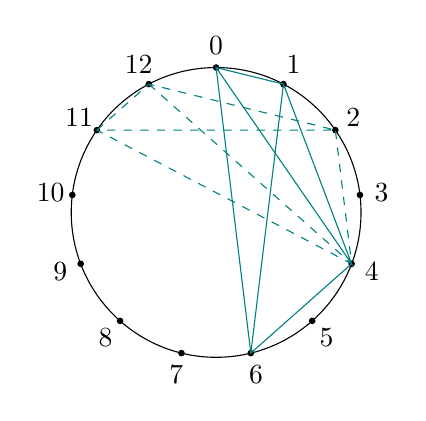
\begin{tikzpicture}[
            scale=0.8,
            baseline=(center_ref.base)]
            \coordinate (center_ref) at (0,0);
            % Draw the circle
            \def\r{2.3}
            \draw (0,0) circle (\r);
            
            % Draw the 13 points and labels
            \foreach \i in {0,...,12} {
                % Calculate angle in degrees (starting from top and going clockwise)
                \pgfmathsetmacro{\angle}{90 - \i * 360 / 13}
                
                % Calculate coordinates on the circle
                \pgfmathsetmacro{\x}{\r*cos(\angle)}
                \pgfmathsetmacro{\y}{\r*sin(\angle)}
                
                % Define the point
                \coordinate (P\i) at: (\x, \y);

                % Place point
                \fill (P\i) circle (1.5pt);
                
                % Calculate label position slightly outside the circle
                \pgfmathsetmacro{\labelx}{1.15 * \x}
                \pgfmathsetmacro{\labely}{1.15 * \y}

                % Place label
                \node at (\labelx, \labely) {\i};
            }
            % Draw a "line"
            \draw[teal]
                (P0) -- (P1) -- (P4) -- (P0) -- (P6) -- (P4);
            \draw[teal] (P1) -- (P6);

            \draw[teal,dashed]
                (P11) -- (P12) -- (P2) -- (P11) -- (P4) -- (P2);
            \draw[teal,dashed] (P12) -- (P4);
        \end{tikzpicture}
    \end{equation}
    Given two indices $i$ and $j$, define the distance $\delta(i,j)$ as the smallest representative in the set $\{0,1,2,\dots,v-1\}$ of either $i-j$ or $j-i$; that is, $\delta(i,j)$ is the minimum number of sides separating vertices $i$ and $j$ in the $v$-gon. In this setting, a rotation around the center $O$ is given by the map $x \mapsto x + r$, where $r\in\Z_v$.
    
    Since $\delta(0,i)=i$ for $1\le i\le(v-1)/2$, the set of all possible positive values of~$\delta$ is
    $$
        \set{1, \dots, (v-1)/2)},
    $$
    which has cardinality $(v-1)/2 = \binom{n+1}{2}$.
    
    Let $X$ denote an $(n+1)$-gon included in the complete $v$-gon. Introduce the set of pairwise distances between its vertices:
    $$
        \Delta(X) = \{\delta(i,j) \mid i \ne j \in X\}.
    $$
    Since $\Delta(X)$ contains at most $\binom{n+1}{2}$ elements, the set
    $$
        \mathcal{D} = \{X : |\Delta(X)| = \tbinom{n+1}{2}\}
    $$
    consists of \textsl{totally irregular} $(n+1)$-gons, i.e., $(n+1)$-gons whose vertices are at pairwise distinct distances.\footnote{Depending on the value of $n$, the set $\mathcal D$ may be empty. As picture \eqref{picture:cyclic-13} shows, $\mathcal D\ne\emptyset$ for $n=3$. However, $\mathcal D$ is known to be empty for $n=6$.}
    
    Assume that $n$ is such that $\mathcal D$ is not empty. Fix one such polygon $R \in \mathcal{D}$, and let $\mathcal{B}$ be the set of its rotations:
    $$
        \blocks = \set{R + r \mid r \in \Z_v}.
    $$
    We claim that the incidence geometry $\igeo$, where $\pts$ is the set of vertices of the $v$-gon and $\incidence$ is the membership relation, defines a projective plane.
    
    To verify axiom~\PP1, take any two distinct points $i$ and $j$. Without loss of generality, we may assume that $\delta(i,j)=j-i$. The definition of $R$ implies that there exist $i', j'\in R$ with $j'-i'=j-i$. Let $R'=R+i-i'$. Since $i'\in R$, $0\in R-i'$ and so $i\in R+i-i'=R'$. Similarly, $j\in R+j-j'=R'$ and so $i,j\in R'$. Now suppose that $i,j\in R'+k$ for some $k$. Since $i$ and $j$ are the only vertices in $R'$ whose distance is $j-i$, and $i+k$ and $j+k$ are at the same distance and belong to $R'+k$, we deduce that $k=0\pmod v$.

    For axiom~\PP2, take any two distinct blocks $R+i$ and $R+j$. Without loss of generality we may assume that $\delta(i,j)=j-i$. Since the vertices of $R$ realize all possible distances between vertices in the $v$-gon, there exist $i',j'\in R$ with $j'-i'=j-i$. Therefore, $j'+i=i'+j\in(R+i)\cap(R+j)$. Now suppose that $k\in(R+i)\cap(R+j)$. We can write $k=k_1+i=k_2+j$ for $k_1,k_2\in R$. Then $k_1-k_2=j-i=j'-i'$, which implies that $k_1=j'$ (and $k_2=i'$). Hence, $k=j'+i$ is the same point we identified before.

    The proof follows from Lemma~\ref{lem:alternative-projective-axiom} because $n+1<n^2+n+1=v$ and so~\hyperref[lem:alternative-projective-axiom]{P3'} is trivially satisfied.
\end{xmpl}

\begin{xmpl}\label{xmpl:triangular-Fano}
    Consider the representation of the Fano plane [cf.~Example~\ref{xmpl:Fano}], and a variant of it, where $\blocks=\set{T+i\mid i\in\Z_7}$, with $T=\set{0,1,3}$.
    $$
        \begin{tikzpicture}[
            scale=0.9,
            every node/.style={font=\small},
            point/.style={draw, circle, fill=black, inner sep=1.5pt, minimum size=4pt},
            line_style/.style={opacity=0.8, color=teal}
          ]
          \coordinate (0) at (90:1.5);
          \coordinate (5) at (210:1.5);
          \coordinate (3) at (330:1.5);
        
          \coordinate (4) at ($(0)!0.5!(5)$);
          \coordinate (2) at ($(5)!0.5!(3)$);
          \coordinate (1) at ($(3)!0.5!(0)$);
        
          \coordinate (6) at (0,0);
        
          \draw (0) -- (4) -- (5);
          \draw (5) -- (2) -- (3);
          \draw[line_style] (3) -- (1) -- (0);
        
          \draw (0) -- (6) -- (2);
          \draw (5) -- (6) -- (1);
          \draw (3) -- (6) -- (4);
          \draw[line_style,dashed] (6) circle (0.75cm);
        
          \node[point,label={[above,font=\small]$0$}] at (0) {};
          \node[point,label={
            [below,yshift=-4pt,
            font=\small]$5$}] at (5) {};
          \node[point,label={
            [below,yshift=-4pt,
            font=\small]$3$}] at (3) {};
          \node[point,label={[left,font=\small]$4$}] at (4) {};
          \node[point,label={
            [below,yshift=-4pt,
            font=\small]$2$}] at (2) {};
          \node[point,label={[right,font=\small]$1$}] at (1) {};
          \node[point, label={
            [label distance=2pt,
            font=\small]left:$6$}] at (6) {};
        \end{tikzpicture}
        %
        \qquad
        %
        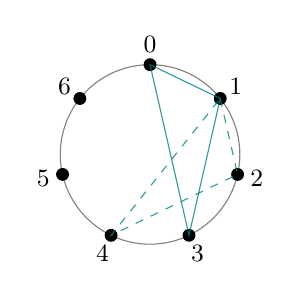
\begin{tikzpicture}[
            scale=0.6,
            every node/.style={font=\small},
            point/.style={circle, fill=black, inner sep=1.5pt, draw=black},
            line_style/.style={opacity=0.8, color=teal}
        ]
        \def\r{1.9};
        \draw[gray] (0,0) circle (\r);
        
        % --- Define the 7 points on a circle ---
        \foreach \i in {0,...,6} {
            % Calculate angle in degrees (starting from top and going clockwise)
            \pgfmathsetmacro{\angle}{90 - \i * 360 / 7}
            
            % Calculate coordinates on the circle
            \pgfmathsetmacro{\x}{\r*cos(\angle)}
            \pgfmathsetmacro{\y}{\r*sin(\angle)}
            
            % Define the point
            \coordinate (p\i) at (\x, \y);
            % Place point
            \node[point] at (p\i) {};
            
            % Calculate label position slightly outside the circle
            \pgfmathsetmacro{\labelx}{1.22 * \x}
            \pgfmathsetmacro{\labely}{1.22 * \y}
            % Place label
            \node at (\labelx, \labely) {\small$\i$};
        }
    
        % --- Draw a couple of lines (the translates of the difference set {0,1,3}) ---
        % Each line is a triangle connecting three points.
        \draw[line_style] (p0) -- (p1) -- (p3) -- cycle;
        \draw[line_style, dashed] (p1) -- (p2) -- (p4) -- cycle;
        \end{tikzpicture}
    $$
    The isomorphism between both representations shows that the Fano plane is cyclic.
\end{xmpl}

\section{Affine Plane}

\begin{defn}
    An incidence geometry $\igeo$ is an \textsl{affine plane} if it satisfies the following properties
    \begin{enumerate}[
        {a}$_\arabic*$,
        ref=\textsc{a$_\arabic*$},
        font=\upshape\scshape]
        \item\label{A1} Every pair of distinct points of $\pts$ is incident with one, and only one, block in~$\blocks$.
        
        \item\label{A2} If $P\nincidence\ell$ for some $P\in\pts$ and $\ell\in\blocks$, then there is a unique $\ell'\in\blocks$ such that $P\incidence\ell'$, and $Q\nincidence\ell'$ whenever $Q\incidence\ell$. 

        \item\label{A3} For every block in $\blocks$ there are at least $2$ distinct points in~$\pts$ incident with the block.

        \item\label{A4} Every point in $\pts$ is incident with, at least, $3$ distinct blocks in~$\blocks$.
    \end{enumerate}
\end{defn}



\begin{rem}\label{rem:projective-line=affine}
    An affine plane can be obtained from a projective plane by removing one line and all the points incident with that line and restricting the incidence relation accordingly.

    As with projective planes, in the case of affine planes we shall use the usual geometric terminology: \textit{a point is on a line}, \textit{two points are joined by a line}, etc.
\end{rem}

\begin{xmpl}\label{xmpl:ag(2,k)}
    Let $\kappa$ be a field. Consider the projective plane $\PG(2,\kappa)$ introduced in Example~\ref{xmpl:pg(2,k)}. If we remove the line whose projective coordinates are $(1:0:0)$, i.e., the projective line with equation $x_0=0$, then the points can be uniquely represented by vectors $(1,x,y)$ and the lines by vectors $(1,a,b)$, and the incidence relation becomes $ax+by+1=0$. This affine plane, denoted by $\AG(2,\kappa)$, is clearly isomorphic to the Euclidean plane $\kappa^2$. If $\kappa=\Fpn$ is a field of $q=p^n$ elements, this plane is denoted $\AG(2,q)$ and it is called the \textsl{affine Galois plane}.
\end{xmpl}

\begin{defn}
    Two lines $\block a$ and $\block b$ in a projective plane are said to be \textsl{parallel}, denoted $\block a\parallel\block b$, if either $\block a=\block b$ or $\block a\cap\block b = \emptyset$.
\end{defn}

\begin{rem}
     The parallel relation is transitive (hence an equivalence relation). Indeed, take $\block a \parallel b$ and $\block b \parallel c$. Suppose, for a contradiction, that $\block a\nparallel c$. In particular, $\block a\ne\block b$ and $\block b\ne\block c$. Pick a point $P$ in $\block a \cap\block c$. Since $\block b$ is disjoint from both $\block a$ and $\block c$, it does not contain $P$. But then we would have two lines, namely $\block a$ and $\block c$, which are disjoint from $\block b$ and incident with $P$, in contradiction with axiom~\ref{A2} applied to $P$ and $\block b$.
\end{rem}

\begin{defn}{\upshape[Projective Closure]}\label{defn:projective-closure}
    Let $\Lambda=\igeo$ be an affine plane. To obtain its \textsl{projective closure}, we adjoin a new block $\ell_\infty$ and a new set of points $\mathcal{P}_\infty$, one for each class in $\blocks/{\parallel}$. Each point $P \in \mathcal{P}_\infty$ is declared incident with the lines in the corresponding parallel class and with $\ell_\infty$. We define the projective closure $\bar\Lambda = (\bar{\pts}, \bar{\blocks}, \bar{\incidence})$, where $\bar{\pts} = \pts \cup \pts_\infty$ and $\bar{\blocks} = \blocks \cup \{\ell_\infty\}$ and $\bar\incidence$ is the extension of $\incidence$ that adds the new incidences involving $\pts_\infty$ and $\ell_\infty$, namely
    $$
    P\mathrel{\bar\incidence} a \iff P\in\pts_\infty
                    \text{ and }a \in P, \text{ or }
                P\in\pts_\infty
                    \text{ and }a=\ell_\infty.
    $$
\end{defn}

\begin{thm}\label{thm:projective-closure}
    The projective closure of an affine plane is a projective plane.
\end{thm}

\begin{proof}
    In what follows we will use the notation of the definition of projective closure.
    \begin{description}
        \item[\rm\textit{$\bar\Lambda$ satisfies} \PP1:] Take two distinct points $A$ and $B$ in $\bar\pts$. If both points are in $\pts$, by \ref{A1}, there is only one line in $\blocks$ incident with both of them. Moreover, $\ell_\infty$ cannot be incident with any of them because it is exclusively incident with points in $\pts_\infty$.

        If $A\in\pts$ and $B\in\pts_\infty$, then \ref{A2} implies that there is precisely one line $\block b$ incident with $A$ in the equivalence class $B$, i.e., such that $A\mathrel{\bar\incidence}b$ and $B\mathrel{\bar\incidence}b$.

        \item[\rm\textit{$\bar\Lambda$ satisfies} \PP2:] Take two distinct lines $\block a$ and $\block b$ in $\bar\blocks$. First consider the case where both lines are in $\blocks$. If there is a point $A$ incident with both of them, no other point $B\ne A$ can be incident with $\block a$ and $\block b$ because of~\PP1. If $\block a\parallel b$, then both define the very same point in $\pts_\infty$. Again, \PP1 ensures that no other point might be in $\block a$ and $\block b$.

        In the case where $\block b=\ell_\infty$, the class of $\block a$ in $\blocks/{\parallel}$ is incident with $\block a$ and with~$\ell_\infty$. Because of \PP1, no other point is incident with both lines.

        \item[\rm\textit{$\bar\Lambda$ satisfies} \PP3:] To see that $\ell_\infty$ is incident with at least $3$ points, it is enough to take $A\in\pts$ and use \PP4 to obtain $3$ incident lines $\block a$, $\block b$ and $\block c$. These lines define three different points in $\pts_\infty$. For a line $\block a\ne\ell_\infty$, take two points incident with $\block a$, as provided by axiom~\ref{A2} and add to them the class of $\block a$ in $\blocks/{\parallel}$.

        \item[\rm\textit{$\bar\Lambda$ satisfies} \PP4:] By \ref{A4}, we only have to consider points in $\pts_\infty$. Let $\block a$ be a line and let $\block a_\infty$ denote its equivalence class in $\blocks/{\parallel}$. Pick a point $A\in\pts$ incident with $\block a$. Let $\block t\in\blocks$ be another line incident with $A$, distinct from~$\block a$. Use axiom~\ref{A3} to pick another point $B\ne A$, incident with $\block t$. By axiom~\ref{A2}, there is a line $\block b\ne\block a$, incident with $B$ and parallel to $\block a$. Then $\block a$, $\block b$, and $\ell_\infty$ are incident with $\block a_\infty$.  
    \end{description}
\end{proof}

\begin{cor}\label{cor:projective-closure}
    If an affine plane\/ $\Lambda$ has a line incident with\/ $n$ points, then:
    \begin{enumerate}[a), font=\upshape]
        \item every line of\/ $\Lambda$ is incident with\/ $n$ points,
        \item every point of\/ $\Lambda$ is incident with\/ $n + 1$ lines,
        \item $\Lambda$ has\/ $n^2$ points and\/ $n^2 + n$ lines in total.
    \end{enumerate}
    The number\/ $n$ is called the \textsl{order} of the affine plane\/ $\Lambda$.
\end{cor}

\begin{proof}
    This is a direct consequence of the theorem and Theorem \ref{thm:order-is-well-defined} applied to the projective closure of~$\Lambda$.
\end{proof}

\begin{thm}
    There exists a projective plane of order\/ $n$ if, and only if, there exists an affine plane of order\/~$n$.
\end{thm}

\begin{proof}
    This is an immediate consequence of Remark~\ref{rem:projective-line=affine} and Corollary~\ref{cor:projective-closure}.
    
\end{proof}

\begin{xmpl}\label{xmpl:AG(2,k)-as-a-complex-plane}
    Let $f$ be an irreducible polynomial of degree two over the field $\kappa$; let $K = \kappa(\iq)$ be the quadratic extension of $\kappa$, where $\iq$ is a root of $f$.  
    The elements of $K$ can be written in the form $a + b\iq$, where $a, b \in \kappa$.
    
    There is a bijection
    \begin{align*}
        \zeta\colon\AG(2,\kappa)&\to K\\
        (x,y)&\mapsto x+y\iq.
    \end{align*}
    This bijection maps the line $(c:a:b)$ onto the subset of $K$
    \[
        \set{x+y\iq \in K\mid ax+by+c= 0}.
    \]  
\end{xmpl}


\begin{thm}
    Consider four points\/ $P_j = (a_j, b_j)$, $1\le j\le 4$, of\/ $\AG(2, \kappa)$, with $P_1\ne P_2$ and $P_3\ne P_4$. Let\/ $z_j=\zeta(P_j) \in K$ in the model of\/ {\upshape Example~\ref{xmpl:AG(2,k)-as-a-complex-plane}}. Then the lines determined by\/ $P_1P_2$ and\/ $P_3P_4$ are parallel if, and only if, there exists\/ $\lambda \in \kappa$ such that
    \[
        z_4 - z_3 = \lambda(z_2 - z_1).
    \]
\end{thm}

\begin{proof}
    Let $(\alpha : \beta : \gamma)$ represent the coefficients of the linear equation
    \[
        \alpha x + \beta y + \gamma = 0.
    \]
    For this projective point to correspond to the line $P_iP_j$, we require
    \[
        \begin{pmatrix}
            a_i & b_i \\
            a_j & b_j
        \end{pmatrix}
        \begin{pmatrix}
            \alpha \\
            \beta
        \end{pmatrix}
        =
        -\gamma
        \begin{pmatrix}
            1 \\
            1
        \end{pmatrix}.
    \]
    Let $d$ denote the determinant of the matrix on the left-hand side (\lhs). Multiplying by the adjugate yields
    \[
        \begin{pmatrix}
            d\alpha \\
            d\beta
        \end{pmatrix}
        =
        -\gamma
        \begin{pmatrix}
            b_j - b_i \\
            a_i - a_j
        \end{pmatrix}.
    \]
    Assuming $d \ne 0$, we may rescale by $d$ and obtain the equation
    \[
        (b_j - b_i)x + (a_i - a_j)y + (a_jb_i - a_ib_j) = 0,
    \]
    which, as a matter of fact, is the equation of the line $P_iP_j$ whenever $P_i \ne P_j$. In particular,
    \begin{align*}
        P_1P_2 \parallel P_3P_4
        &\iff
            \det\begin{pmatrix}
                b_2 - b_1 & a_1 - a_2 \\
                b_4 - b_3 & a_3 - a_4
            \end{pmatrix}
            = 0 \\
        &\iff\exists\,\lambda\in\kappa^*\;\text{such that }
            \begin{cases}
                b_4 - b_3 = \lambda(b_2 - b_1)\\
                a_3 - a_4 = \lambda(a_1 - a_2)
            \end{cases}\\
        &\iff z_4 - z_3 = \lambda(z_2 - z_1).
    \end{align*}
\end{proof}

\begin{cor}
    Three distinct points, $P_j = (a_j, b_j)$, $1\le j\le 3$, of\/ $\AG(2,q)$ are collinear if, and only if,
    \begin{equation}\label{eq:z-diff}
        (z_2 - z_3)^{q-1} = (z_2 - z_1)^{q-1}
    \end{equation}
    holds for the elements\/ $z_j = a_j + b_j i \in \Fq[q^2]$.
\end{cor}

\begin{proof}
    By the Theorem applied to case $P_4=P_2$, we see that the three points are collinear if, and only if, there exists $\lambda\in\Fq$ such that
    $$
        z_2-z_3 = \lambda(z_2-z_1).
    $$
    Since $\lambda^{q-1}=1$, the \textit{only if} part is clear. Now suppose that equality \eqref{eq:z-diff} is satisfied and let $\lambda=(z_2-z_3)/(z_2-z_1)$. Then $\lambda\in\kappa^*$, since it satisfies the polynomial equation $x^{q-1}-1=0$, whose solutions all lie in~$\kappa$.


\end{proof}

\begin{xmpl}\label{xmpl:affine-moulton}{\upshape[Affine Moulton Plane]}
    The \textsl{affine Moulton plane} has the same points as the Euclidean plane, but it bends all lines with positive slope to halve their slope as they cross from the lower- (below the $x$-axis) to the upper-half plane (above the axis). 
    $$
        \begin{tikzpicture}[scale=0.65]
            % Axis
            \draw[->,very thick] (-3.5,0) -- (4.3,0) node[right] {$x$};
            
            % Line a: negative slope
            \draw[name path=a] (-3,2.5) -- (3,-0.4) node[right] {$\block a$};
            
            % Line b: negative slope
            \draw[name path=b] (-3,0.5) -- (3,-1.5) node[right] {$\block b$};
            
            % Line v: vertical line
            \draw[name path=v] (1,-2.5) -- (1,3) node[above]{$\block v$};
            
            % Line d: positive slope with bending
            \def\x0{-3}
            \def\y0{-2}
            \def\xi{0.3}
            \def\xh{3}
            \draw[name path=d1] (\x0,\y0) -- (\xi,0);
            \pgfmathsetmacro{\m}{-\y0/(\xi-\x0}
            \pgfmathsetmacro{\mh}{\m/2}
            
            % Define the y-intercept (b value)
            \pgfmathsetmacro{\b}{\y0-\m*\x0}
            \pgfmathsetmacro{\bh}{-\mh*\xi}
            
            % Draw the line using two points
            \draw[name path=d2] (\xi,0) -- (3,{\m/2*3+\b}) node[right]{$\block d$};
            \draw[name path=ds,dashed] (\xi,0) -- (1.6,{\m*1.6+\b});
            
            % Line e: positive slope with bending
            \def\x0{-1.2}
            \def\y0{-2.5}
            \def\xi{-0.5}
            \def\xh{0.1}
            \draw[name path=e1] (\x0,\y0) -- (\xi,0);
            \pgfmathsetmacro{\m}{-\y0/(\xi-\x0)}
            \pgfmathsetmacro{\mh}{\m/2}
            
            % Define the y-intercept (b value)
            \pgfmathsetmacro{\b}{\y0-\m*\x0}
            \pgfmathsetmacro{\bh}{-\mh*\xi}
            
            % Draw the line using two points
            \draw[name path=e2] (\xi,0) -- (0.4,{\mh*0.4+\bh}) node[above,xshift=3pt]{$\block e$};
            \draw[name path=ds,dashed] (\xi,0) -- (0.01,{\m*0.01+\b});
        \end{tikzpicture}
    $$
    In the picture, lines $\block a$, $\block b$ and $\block v$ are the same in both the Moulton plane and the Euclidean plane. However, lines $\block e$ and $\block d$, which belong to the Moulton plane, differ from the Euclidean ones in that they have their slopes halved in the upper half-plane.

    In order to verify axiom~\ref{A1} in the Moulton plane it is enough to consider the case of two points $(x_0,y_0)$ and $(x_1,y_1)$ such that $x_0<x_1$ and $y_0<0<y_1$.
    \begin{equation}\label{picture:moulton-m}
        \begin{tikzpicture}[
            scale=1,
            baseline=(center_ref.base)
            ]
            \coordinate (center_ref) at (0,0);
            % Axis
            \draw[->,very thick] (-3.5,0) -- (4.3,0) node[right] {$x$};
            
            % Line d: positive slope with bending
            \def\x0{-3.0}
            \def\y0{-2}
            \def\u{1.0}
            \def\v{0.7}
            \pgfmathsetmacro{\xi}{(2*\v*\x0-\y0*\u)/(2*\v-\y0)}
            \draw[name path=d1] (\x0,\y0) -- (\xi,0);
            \pgfmathsetmacro{\mh}{\v/(\u-\xi)};
            \pgfmathsetmacro{\m}{\mh*2};
            
            % Define the y-intercept (b value)
            \pgfmathsetmacro{\b}{\y0-\m*\x0}
            \pgfmathsetmacro{\bh}{\v-\mh*\u}

            % Draw the line using two points
            \draw[name path=d2] (\xi,0) -- (2.5,{\mh*2.5+\bh}) node[right]{$\block d$};
            \draw[name path=ds,dashed] (\xi,0) -- (1.6,{\m*1.6+\b});

            \coordinate (A) at ({\x0+1},{\m*(\x0+1)+\b});
            \draw[fill=black] (A) circle (2pt) node[below right] at (A) {$(x_0,y_0)$};

            \coordinate (B) at ({\xi+2},{\mh*(\xi+2)+\bh});
            \draw[fill=black] (B) circle (2pt) node[below right]{$(x_1,y_1)$};

            \coordinate (C) at ({\xi},0);
            \draw[fill=white] (C) circle (2pt) node[below,yshift=-3pt]{$c$};
        \end{tikzpicture}        
    \end{equation}
    Our goal is to determine the value of $c$ and the slope $m$ of the line passing through $(x_0, y_0)$ and $(c, 0)$.  
    To that end, we consider the system
    \begin{align}\label{eq:moulton-m}
        m &= \frac{-y_0}{c-x_0},\nonumber\\
        \frac{m}{2} &= \frac{y_1}{x_1-c}.
    \end{align}
    From these equations, we deduce
    \[
        c y_0 - y_0 x_1 = 2c y_1 - 2y_1 x_0,
    \]
    which leads to
    \[
        c = \frac{2y_1x_0 - y_0x_1}{2y_1 - y_0}.
    \]
    Now that $\block c$ is known, the value of $m$ follows from the first equation.

    To verify axiom~\ref{A2}, observe that two lines fail to meet if, and only if, they do not intersect in either the lower or the upper half-plane. This occurs precisely when they are both horizontal, both vertical, or share the same slope in the corresponding half-plane---and therefore, in both half-planes.

    axioms~\ref{A3} and \ref{A4} are trivial in this incidence geometry.
\end{xmpl}

\begin{xmpl}\label{xmpl:parabola-plane}{\upshape[Parabolic Affine Plane]}
    Starting from the Euclidean plane, this model uses the same points and takes as lines all the translations of the function $x\mapsto x^2$, plus the translations of the vertical line with equation $x=0$.
    $$
        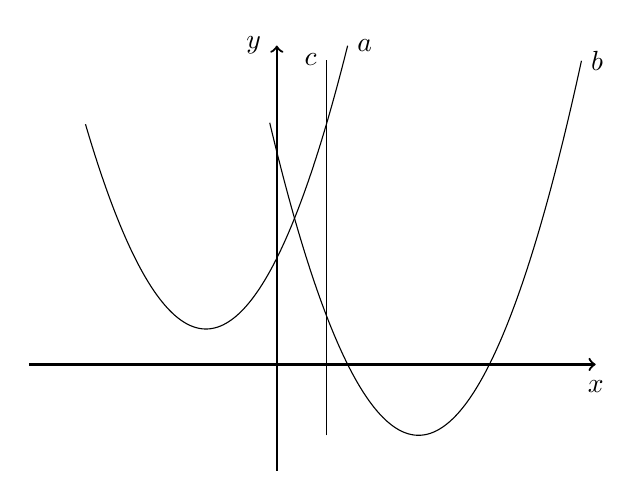
\begin{tikzpicture}[scale=0.9]
            % Axes
            \draw[->,thick] (-3.5,0) -- (4.5,0) node[below,yshift=-2pt] {$x$};
            \draw[->,thick] (0,-1.5) -- (0,4.5) node[left,xshift=-2pt] {$y$};
        
            % Vertical line
            \draw (0.7,-1) -- (0.7,4.3) node[left] {$\block c$};
        
            % First parabola: y = (x-2)^2 - 1
            \draw[domain=-0.1:4.3, samples=100, smooth, variable=\x]
                plot ({\x}, {(\x-2)*(\x-2) - 1}) node[right] {$\block b$};
        
            % Second parabola: y = (x+1)^2 + 1
            \draw[domain=-2.7:1, samples=100, smooth, variable=\x]
                plot ({\x}, {(\x+1)*(\x+1) + 0.5}) node[right] {$\block a$};
        \end{tikzpicture}
    $$
    Let $f(x)=x^2$. Given two points $(x_0,y_0)$ and $(x_1,y_1)$, to verify axiom~\ref{A1}, i.e., that they define a unique parabolic line, it is enough to show that the equations
    $$
        y_0=f(x_0+a)+b,\quad y_1=f(x_1+a)+b
    $$
    have only one solution $(a,b)$ when $x_0\ne x_1$. This translates into
    $$
        y_0-b=(x_0+a)^2\quad\text{and}\quad y_1-b=(x_1+a)^2,
    $$
    i.e.,
    $$
        y_1-y_0=(x_0+x_1+2a)(x_1-x_0)\quad\text{and}\quad
            b=y_0-(x_1+a)^2.
    $$
    Clearly, there is only one solution because we can solve the first for $a$ and then get $b$ from the second.

    To verify axiom~\ref{A2}, it suffices to prove it when the block is $y=x^2$ and the point $(x_0,y_0)$ is such that $y_0\ne x_0^2$. In this case, we must verify that there is a unique pair $(a,b)$ with $y_0=(x_0-a)^2+b$ and $x^2\cap (x-a)^2+b=\emptyset$. One solution is $(a,b)=(0,y_0-x_0^2)$. Moreover, any other solution $(c,d)$ would satisfy $(x_0-c)^2+d=y_0$ and $x^2\cap(x-c)^2+d=\emptyset$. But this can only happen if $c=0$, since otherwise, $2cx=d-c^2$ could be solved for $x$. Thus, $c=0$ and therefore $d=y_0-x_0^2=b$, which makes $(c,d)$ identical to the solution~$(a,b)$.

    Axioms~\ref{A3} and \ref{A4} are trivial.
\end{xmpl}

\begin{xmpl}{\upshape[Latin Squares]}
    A \textsl{Latin square of order} $n$ is an $n\times n$ matrix in which each row and each column is a permutation of $\set{0,\dots,n-1}$.
    
    More precisely, let $A = (a_{ij})$ be an $n \times n$ matrix with entries in $\nset[0]{n-1}$. Define its \textsl{entry function}
    \begin{align*}
        \ev A\colon\nset n\times\nset n&\to\nset[0]{n-1}\\
        (i,j)&\mapsto a_{ij}.
    \end{align*}
    Then $A$ is a Latin square if, for every $i,j\in\nset n$, the slice functions $\ev A(\,\cdot\,,j)$ and $\ev A(i,\,\cdot\,)$ are bijections from $\nset n$ to $\nset[0]{n-1}$. Since the domain and codomain of the slice functions are finite sets of the same cardinality, bijection, injection, and surjection are equivalent in this context.
    
    This means that every $i\in\nset[0]{n-1}$ appears exactly once in each row and each column of $A$. For example, the following matrix is a Latin square of order $4$:
    \[
        \begin{bmatrix}
        0 & 1 & 2 & 3 \\
        1 & 0 & 3 & 2 \\
        2 & 3 & 0 & 1 \\
        3 & 2 & 1 & 0
    \end{bmatrix}
    \]
    If $\sigma$ is a permutation of $\nset[0]{n-1}$, then the matrix $A^\sigma = (\sigma(a_{ij}))$ is also a Latin square of order $n$, since
    \[
        \ev{A^\sigma}(\,\cdot\,,j) = \sigma \circ \ev A(\,\cdot\,,j)
        \quad\text{and}\quad
        \ev{A^\sigma}(i,\,\cdot\,) = \sigma \circ \ev A(i,\,\cdot\,).
    \]
    Two Latin squares $A = (a_{ij})$ and $B = (b_{ij})$ are said to be \textsl{orthogonal}, written $A \perp B$, if the pairs $(a_{ij}, b_{ij})$ are all distinct. Equivalently, the map
    \begin{align*}
        (\ev A,\ev B)\colon\nset n\times\nset n
            &\to\nset[0]{n-1}\times\nset[0]{n-1}\\
            (i,j)&\mapsto(a_{ij}, b_{ij})
    \end{align*}
    is an injection. Again, bijectivity is equivalent here to injectivity or surjectivity.
    
    Here is an example of two orthogonal Latin squares of order $4$:
    \[
        \begin{bmatrix}
        0 & 1 & 2 & 3 \\
        1 & 0 & 3 & 2 \\
        2 & 3 & 0 & 1 \\
        3 & 2 & 1 & 0
        \end{bmatrix}
        \quad
        \begin{bmatrix}
        0 & 1 & 2 & 3 \\
        2 & 3 & 0 & 1 \\
        3 & 2 & 1 & 0 \\
        1 & 0 & 3 & 2
        \end{bmatrix}
        \quad\longrightarrow\quad
        \begin{matrix}
        (0,0) & (1,1) & (2,2) & (3,3) \\
        (1,2) & (0,3) & (3,0) & (2,1) \\
        (2,3) & (3,2) & (0,1) & (1,0) \\
        (3,1) & (2,0) & (1,3) & (0,2)
        \end{matrix}
    \]
    Let $\sigma$ be a permutation of $\nset[0]{n-1}$ and $A$, $B$ Latin squares of order $n$. Then
    \begin{equation}\label{eq:latin-orthogonal}
        A \perp B \iff A^\sigma \perp B
        \tag{$\star$}
    \end{equation}
    because
    \[
        (\ev{A^\sigma}, \ev B) = (\sigma \times \id) \circ (\ev A, \ev B).
    \]
    A set $\set{A_1, A_2, \dots, A_m}$ of Latin squares of order $n$ is said to be a set of \textsl{mutually orthogonal Latin squares} (abbreviated $\mols$) if $A_h\perp A_k$ for every pair $h\ne k$.
    
    For example, the following Latin squares form a $\mols$:
    \[
        A =
        \begin{bmatrix}
        0 & 1 & 2 & 3 & 4 \\
        1 & 2 & 3 & 4 & 0 \\
        2 & 3 & 4 & 0 & 1 \\
        3 & 4 & 0 & 1 & 2 \\
        4 & 0 & 1 & 2 & 3
        \end{bmatrix}
        \quad
        B =
        \begin{bmatrix}
        0 & 2 & 4 & 1 & 3 \\
        1 & 3 & 0 & 2 & 4 \\
        2 & 4 & 1 & 3 & 0 \\
        3 & 0 & 2 & 4 & 1 \\
        4 & 1 & 3 & 0 & 2
        \end{bmatrix}
        \quad
        C =
        \begin{bmatrix}
        0 & 3 & 1 & 4 & 2 \\
        1 & 4 & 2 & 0 & 3 \\
        2 & 0 & 3 & 1 & 4 \\
        3 & 1 & 4 & 2 & 0 \\
        4 & 2 & 0 & 3 & 1
        \end{bmatrix}
    \]
\end{xmpl}

\begin{prop}
    Let\/ $N(n)$ denote the maximal number of\/ $\mols$ of order\/~$n$. Then, $N(n)\le n-1$.
\end{prop}

\begin{proof}
    Let $\set{A_1,\dots,A_m}$ be a $\mols$ of order $n$. According to \eqref{eq:latin-orthogonal} we may assume, without loss of generality, that the first row of every matrix is $(0,1,\dots,n-1)$. This has two consequences
    \begin{enumerate}[i)]
        \item $\ev{A_k}(1,1)=0$, for $k=1,\dots,m$, and
        \item $(\ev{A_h},\ev{A_k})(1,j)=(j-1,j-1)$, for $1\le h,k\le m$ and $j=1,\dots,n$. 
    \end{enumerate}
    Now consider the set $E=\set{\ev{A_k}(2,1)\mid 1\le k\le m}$. Clearly, ii) implies that the map
    \begin{align}\label{map:eval-21}
        \ev{}\colon\nset m&\to E\\
        k&\mapsto\ev{A_k}(2,1)\nonumber
    \end{align}
    is injective. In particular, $m\le|E|$. Since $0\notin E$ by i), we have $E\subseteq\nset{n-1}$. Hence, $m\le|E|\le n-1$.

\end{proof}

\begin{defn}
    A set of $\mols$ of order $n$ is \textsl{complete} when it has $n-1$ elements.
\end{defn}

\begin{lem}\label{lem:mols-P1}
    Let $\set{L_1,\dots,L_{n-1}}$ be a complete set of $\mols$ of order $n$, where $L_m=(b^m_{ij})_{1\le i,j\le n}$. Then, given $1\le x,y,a,b\le n$, with $x\ne a$ and $y\ne b$, there exists one, and only one, $m$ such that $b^m_{xy}=b^m_{ab}$.
\end{lem}

\begin{proof}
    According to \eqref{eq:latin-orthogonal} we may assume, without loss of generality, that the $x$th row of every matrix is $(0,1,\dots,n-1)$. Thus, $b^m_{xj}=j-1$ for all $m$ and all $j$.
    The map
    \begin{align}\label{map:ev-ab}
        \ev{}\colon\nset{n-1}
            &\to\nset[0]{n-1}\setminus\set{b-1}\\
        m&\mapsto \ev{A_m}(a,b)
    \end{align}
    is well-defined because $a\ne x$ and so $\ev{A_m}(a,b)\ne\ev{A_m}(x,b)=b-1$.
    
    The same reasoning used to deduce the injectivity of \eqref{map:eval-21} shows that~$\ev{}$ is injective: if $e$ is the common value of $\ev{A_r}(a,b)$ and $\ev{A_s}(a,b)$ then $(e,e)$ would be repeated twice in the set of pairs $(\ev{A_r}(i,j),\ev{A_s}(i,j))$, the second being for $(i,j)=(x,e+1)$. In consequence, $\ev{}$ is a bijection and so there is exactly one value of $m$ such that $b^m_{xy}=b^m_{ab}$, as desired.
    
\end{proof}

\begin{thm}\label{thm:mols-equivalence}
    Let\/ $n\ge2$. Then there exists a projective plane of order\/ $n$ if, and only if, there exists a complete set of $\mols$ of order\/~$n$.
\end{thm}

\begin{proof}
    Let $\set{L_1,\dots,L_{n-1}}$ be a complete set of $\mols$. For $1\le m<n$, put $L_m=(b^m_{ij})_{1\le i,j\le n}$. We define an incidence geometry $\Pi=\igeo$ as follows.
    
    \small
    \textit{Points:}
    $$
        \pts=\set{(x,y)\mid 1\le x,y\le n}\cup\set{(m)\mid0\le m<n}\cup\set{(\infty)},
    $$
    where
    \begin{enumerate}[-]
        \item $(x, y)$: These are the ``ordinary'' or affine points. Think of them like the points on a standard Cartesian grid, where $x$ and $y$ are coordinates. There are $n^2$ such points.
        \item $(m)$: These are $n$ additional points, representing points at infinity for lines with finite slopes. Each $m$ corresponds to a unique slope.
        \item $(\infty)$: This is one special point, representing the point at infinity for vertical lines.
    \end{enumerate}
    \textit{Lines:}
    $$
        \blocks = \set{[m,b]\mid 0\le m,b<n} \cup \set{[a]\mid 0\le a<n} \cup \set{[\infty]},
    $$
    where
    \begin{enumerate}[-]
        \item $[m, b]$: These are $n^2$ lines, representing ``ordinary'' lines with finite slopes. Each $m$ represents the slope and each $b$ the ``$y$-intercept''.
        \item $[a]$: These are $n$ additional lines, representing vertical lines. Each $a$ corresponds to an $x$-coordinate.
        \item $[\infty]$: This is one special line, representing the line at infinity.
    \end{enumerate}
    \textit{Incidence:}
    \begin{enumerate}[1.]
        \item Affine Points and Ordinary Lines (forming an Affine Plane):
        \begin{enumerate}[-]
            \item An affine point $(x, y)$ is incident with a vertical line $[a]$ if and only if $x = a$.
            \begin{enumerate}[$\to$]
                \item This is like saying a point $(x,y)$ is on the vertical line $x=a$ if its $x$-coordinate is $a$.
            \end{enumerate}
            \item An affine point $(x, y)$ is incident with a horizontal line $[0, b]$ if and only if $y = b$.
            \begin{enumerate}[$\to$]
                \item This is like saying a point $(x,y)$ is on the horizontal line $y=b$ if its $y$-coordinate is $b$.
            \end{enumerate}
            \item For lines with non-zero slope $m$, an affine point $(x, y)$ is incident with all the lines $[m, b]$ precisely when $b = b^m_{xy}$.
            \begin{enumerate}[$\to$]
                \item This is the core of the $\mols$ connection. For each possible slope $m$ (excluding 0 and vertical), there's a Latin square $L_m$. The value $b^m_{xy}$ essentially acts as the ``$y$-intercept'' for a line of slope $m$ passing through $(x, y)$. The orthogonality of the Latin squares ($\mols$ property) is crucial here to ensure that any two distinct lines $[m_1, b_1]$ and $[m_2, b_2]$ (with $m_1, m_2 \ne 0$, and not both $m_1=m_2$ and $b_1=b_2$) intersect at exactly one affine point.
            \end{enumerate}
        \end{enumerate}
        \item Affine Points and the Line at Infinity:
        \begin{enumerate}[-]
            \item An affine point $(x, y)$ is never incident with the line $[\infty]$.
            \begin{enumerate}[$\to$]
                \item Affine points are ``finite'' and do not lie on the ``line at infinity''.
            \end{enumerate}
        \end{enumerate}
        \item Points at Infinity and Ordinary Lines:
        \begin{enumerate}[-]
            \item A point at infinity $(m)$ is incident with a line $[s,b]$ if, and only if, $s = m$.
            \begin{enumerate}[$\to$]
                \item The point $(m)$ represents the slope $m$. So, any line with slope $s$ passes through the point at infinity corresponding to $s$. This links parallel lines (which share a slope $m$) to a common ``ideal point''~$(m)$.
            \end{enumerate}
            \item A point at infinity $(m)$ is never incident with a vertical line $[a]$.
            \begin{enumerate}[$\to$]
                \item Points $(m)$ represent finite slopes, while vertical lines have an infinite slope.
            \end{enumerate}
        \end{enumerate}
        \needspace{2\baselineskip}
        \item The Special Point $(\infty)$ and Ordinary Lines:
        \begin{enumerate}[-]
            \item The point $(\infty)$ is incident with all lines of type $[a]$ (vertical lines).
            \begin{enumerate}[$\to$]
                \item The point $(\infty)$ represents the ``vertical direction''. All vertical lines are considered parallel and thus meet at this single point at infinity.
            \end{enumerate}
            \item The point $(\infty)$ is not incident with lines of type $[m, b]$ (lines with finite slopes).
            \begin{enumerate}[$\to$]
                \item This reinforces that $(\infty)$ is specifically for vertical lines, not those with finite slopes.
            \end{enumerate}
        \end{enumerate}
        \item Points at Infinity and the Line at Infinity:
        \begin{enumerate}[-]
            \item Any point at infinity $(m)$ is always incident with the line $[\infty]$.
            \begin{enumerate}[$\to$]
                \item All points at infinity (representing slopes, both finite and vertical) lie on the ``line at infinity''.
            \end{enumerate}
            \item The special point $(\infty)$ is incident with the line $[\infty]$.
            \begin{enumerate}[$\to$]
                \item The point at infinity for vertical lines also lies on the line at infinity.
            \end{enumerate}
        \end{enumerate}
    \end{enumerate}
    \normalsize

    Let's now prove that $\Pi$ satisfies axioms~\PP1, \PP2 and \hyperref[lem:alternative-projective-axiom]{P3'}.

    \begin{description}
        \item[\rm P1.] Take two distinct points $P\ne Q$. There are several cases.
        
        \textit{Case\/ }1: $P=(x,y)$ and $Q=(a,b)$. If $x=a$, then $y\ne b$ and so $P,Q\incidence {[a]}$ and $P\nincidence {[0,b]}$. If $y=b$, then $x\ne a$ and so $P,Q\incidence{[0,b]}$ and $P\nincidence{[0,b]}$. If $x\ne a$ and $y\ne b$, then $b^m_{x,y}=b^m_{a,b}$ for precisely one value of $m$, as shown in Lemma~\ref{lem:mols-P1}.

        \textit{Case\/ }2: $P=(x,y)$ and $Q=(m)$. The line $[m,b^m_{xy}]$ is incident with both $P$ and $Q$. It is the only one, by part~3.~``Points at Infinity and Ordinary Lines'' above.

        \textit{Case\/ }3: $P=(x,y)$ and $Q=(\infty)$. The ``vertical''line $[x]$ is the only one that joins $P$ and $Q$.

        \textit{Case\/ }4: $P=(m_1)$ and $Q=(m_2)$. These two points are incident with~$[\infty]$ (and no other line).

        \textit{Case\/ }5: $P=(m_1)$ and $Q=(\infty)$. Idem Case 4 just considered.

        \item[\rm P2.] Take two distinct lines $\block a$ and $\block b$. There are several cases.

        \textit{Case\/ }1: $\block a=[r,a]$ and $\block b=[s,b]$. If $r=s$ and their common value is $m$, then both lines meet at the infinite point $(m)$, and no other. If $r\ne s$ and $r=0$, both lines meet at $(x,a)$ where $x$ is the only index such that $b^s_{xa}=b$.

        \textit{Case\/ }2: $\block a=[r,a]$ and $\block b=[b]$. If $r=0$, both lines meet (exclusively) at $(b,a)$. If $r\ne0$, both lines meet at $(b,y)$, where $y$ is the only index such that $b^r_{by}=a$.

        \textit{Case\/ }3: $\block a=[r,a]$ and $\block b=[\infty]$. Then both lines meet at $(r)$.

        \textit{Case\/ }4: $\block a=[a]$ and $\block b=[b]$. Here the common point of incidence is $(\infty)$.

        \textit{Case\/ }5: $\block a=[a]$ and $\block b=[\infty]$. These lines meet (only) at the vertical direction~$(\infty)$.

        \item[\rm P3'.] We may assume that the first row of every matrix is $(0,\dots,n-1)$. The points $(1,1)$, $(1,2)$, $(2,1)$ and $(2,2)$ are in general position:
        \begin{itemize}
            \item[-] $(1,1)(1,2)=[1]$ and $(2,1),(2,2)\notin[1]$,
            \item[-] $(1,1)(2,1)=[0,1]$ and $(1,2),(2,2)\notin[0,1]$,
            \item[-] $(1,1)(2,2)=[m,0]$, where $m$ is the only index such that $b^m_{22}=b^m_{11}=0$ (see Lemma~\ref{lem:mols-P1}). Moreover, $(1,2)\notin[m,0]$ because $b^m_{12}=1\ne0$, and $(2,1)\notin[m,0]$ because $b^m_{21}\ne b^m_{11}=0$,
            \item[-] $(1,2)(2,1)=[m,1]$, where $m$ is the only index such that $b^m_{21}=1$ (Lemma~\ref{lem:mols-P1}). Moreover, $(1,1)\notin[m,1]$ because $b^m_{11}=0\ne1$, and $(2,2)\notin[m,1]$ because $b^m_{22}\ne b^m{12}=1$.
            \item[-] $(2,1)(2,2)=[2]$ and $(1,1),(1,2)\notin[2]$.
        \end{itemize}
    \end{description}

    \medskip

    For the converse, suppose that $\Pi=\igeo$ is a projective plane of order~$n$. Fix a line $\ell$ to be the line at infinity in the affine plane $\Lambda=(\pts_\Lambda,\blocks_\Lambda,\incidence_\Lambda)$ obtained by removing it. Additionally, fix two points $X\ne Y$ incident with $\ell$. These will, respectively, play the roles of the horizontal and vertical directions. More precisely, define
    \begin{align*}
        \pl(X)\setminus\set\ell
            &= \set{\block h_1,\dots,\block h_n},\\
        \pl(Y)\setminus\set\ell
            &= \set{\block v_1,\dots,\block v_n}.
    \end{align*}
    Then the map
    \begin{align*}
        \lambda\colon\nset n\times\nset n &\to \pts_\Lambda\\
        (i,j) &\mapsto \block h_i\wedge\block v_j
    \end{align*}
    is well-defined because\/ $\block h_i\wedge\block v_j\nincidence\ell$. We claim that $\lambda$ is injective. Suppose, towards a contradiction, that\/ $\block h_i\wedge\block v_j=\block h_{i'}\wedge\block v_{j'}$, and let\/ $A$ denote the common point. Then\/ $A\incidence\block h_i,\block h_{i'}$, which forces\/ $A=X$ unless\/ $i=i'$. But\/ $A\ne X$ by construction, hence\/ $i=i'$. Similarly, $j=j'$, and injectivity is established. By cardinality,~$\lambda$ is a bijection.
    
    Fix an enumeration
    $$
        \tr(\ell)\setminus\set{X,Y}
            =\set{M_1,\dots,M_{n-1}}
            \stackrel\cong\longrightarrow\nset{n-1}.
    $$
    For every $m\in\nset{n-1}$, fix an enumeration of $\pl(M_m)\setminus\set\ell$
    \begin{align*}
    \pl(M_m)\setminus\set\ell
        =\set{\block m_1,\dots,\block m_n}
        &\stackrel{\sigma_m}\longrightarrow\nset[0]{n-1}\\
    \block m_k&\longmapsto k-1.
    \end{align*}
    For each $m\in\nset{n-1}$ define the $n\times n$ matrix $L_m$ with coefficients in $\nset[0]{n-1}$ by $L_m=\sigma_m\circ\iota_m\circ\lambda$, as shown in the following diagram
    $$
        \begin{tikzcd}
            \nset n\times\nset n
                    \arrow[r,"L_m"]
                    \arrow[d,"\lambda"']
                &\nset[0]{n-1}\\
            \pts_\Lambda
                    \arrow[r,"\iota_m"']
                &{\set{\block m_1,\dots,\block m_n}}
                    \arrow[u,"\sigma_m"']
        \end{tikzcd}
    $$
    where $\iota_m(A)=\block m_k\iff A\incidence\block m_k$.

    \textbf{Each $L_m$ is a Latin square.} To verify this it suffices to show that, for each pair\/ $(i,j)$, the restrictions\/ $L_m(i,\,\cdot\,)$ and\/ $L_m(\,\cdot\,,j)$ are injective. Since\/ $\sigma_m$ is a bijection, it is enough to check that the compositions\/ $\iota_m\circ\lambda(i,\,\cdot\,)$ and\/ $\iota_m\circ\lambda(\,\cdot\,,j)$ are injections.

    Suppose, for contradiction, that\/ $A\ne B$ are finite points both incident with\/ $\block h_i$ (respectively,\/ $\block v_j$) and with some\/ $\block m_k$. Then\/ $AB=\block h_i$ (respectively,\/ $\block v_j$) and also\/ $AB=\block m_k$, contradicting the definitions of\/ $M$ and\/ $X$ (respectively,\/ $Y$).

    
    \textbf{If $h\ne k$ then $L_h\perp L_k$.} By cardinality it is enough to show that the map
    \begin{align*}
        (L_h,L_k)\colon\nset n\times\nset n
            &\to\nset[0]{n-1}\times\nset[0]{n-1}\\
        (i,j)&\mapsto(L_h(i,j),L_k(i,j))
    \end{align*}
    is injective. Suppose
    $$
        L_h(i,j)=L_h(i',j')\quad\text{and}\quad
        L_k(i,j)=L_k(i',j'),
    $$
    i.e.,
    \begin{align*}
        A%\hphantom{'}
            = \block h_i\wedge\block v_j\incidence\block m_h,\quad
        A' 
            =\block h_{i'}\wedge\block v_{j'}\incidence\block m_h,\\
        A%\hphantom{'}
            =\block h_i\wedge\block v_j\incidence\block m_k,\quad
        A'
            =\block h_{i'}\wedge\block v_{j'}\incidence\block m_k.
    \end{align*}
    Since $A$ (as well as $A'$) belongs in $\pts_\Lambda$ and $\block m_h\wedge\block m_k=M\incidence\ell$, we arrive at a contradiction.

    The last two facts establish that $\set{L_1,\dots,L_{n-1}}$ is a $\mols$.

\end{proof}

%\newcommand{\iu}{{\mkern1mu i\mkern1mu}}
\newcommand{\iu}{\sqrt{-1}}
\begin{prop}
    Let\/ $\Z[\iu]$ be the ring of Gaussian integers. If\/ $p\in\Z$ is an odd prime, then the following are equivalent
    \begin{enumerate}[a),font=\upshape]
        \item $p\equiv1\pmod 4$
        \item $x^2+1$ is reducible in $\Z/p\Z[x]$
        \item $p$ is not prime in\/ $\Z[\iu]$
        \item $p=a^2+b^2$ for some $a,b\in\Z$.
    \end{enumerate}
\end{prop}

\begin{proof}
    See \citep{LC-Hopf}, Prime Ideals.
\end{proof}

\begin{cor}\label{cor:sum-of-squares}
    A positive integer\/ $n$ is the sum of two perfect squares if, and only if, each prime divisor of the form\/ $4k+3$ has an even exponent in the prime factorization of\/~$n$.
\end{cor}

\begin{proof}
    Write
    $$
        n=2^mp_1^{e_1}\cdots p_h^{e_h}q_1^{d_1}\cdots q_k^{d_k},
    $$
    where every $p_i\equiv1\pmod4$ and every $q_j\equiv3\pmod4$. By the proposition, each $q_j$ is prime in $\Z[\iu]$ and we have $p_i=a_i^2+b_i^2=N^2(a_i+b_i\iu)$. Therefore, using the fact that $N^2$ is multiplicative, we obtain
    \begin{equation}
        p_1^{e_1}\cdots p_h^{e_h}=N^2(a+b\iu)=a^2+b^2,
            \tag{$\star$}
    \end{equation}
    where
    $$
        a+b\iu=(a_1+b_1\iu)^{e_1}\cdots(a_h+b_h\iu)^{e_h}.
    $$
    Now suppose that $n=u^2+v^2=(u+v\iu)(u-v\iu)$ for some $u,v\in\Z$. Since each $q_j$ is prime in $\Z[\iu]$, we deduce that $q_j\mid u+v\iu$ or $q_j\mid u-v\iu$. Hence, in any case, $q_j\mid u$ and $q_j\mid v$. Thus, $q_j^2\mid u^2,v^2$. Dividing $u^2$ and $v^2$ by the maximum exponent of $q_j^2$ that divides both, we obtain a factor of $n$ that is also a sum of two squares and that is not divisible by any prime $q_j$. This means that $d_j$ is even.

    Now suppose that each $d_j$ is even and let's verify that $n$ is a sum of two squares. From ($\star$) we deduce that
    $$
        n=2^e(u^2+v^2),
    $$
    for some integers $u$ and $v$, where $e=0$ or $e=1$. In the case $e=0$, the conclusion is obvious. Suppose that $e=1$. Then we would have
    \begin{align*}
        n &= 2(u^2+v^2)\\
            &= (1+\iu)(u+v\iu)(1-\iu)(u-v\iu)\\
            &= (u-v+(u+v)\iu)(u-v-(u+v)\iu)\\
            &= (u-v)^2+(u+v)^2.
    \end{align*}
\end{proof}

\begin{cor}\label{cor:sum-of-two-rational-squares}
    If a positive integer is the sum of two rational squares, then it is the sum of two integer squares.
\end{cor}

\begin{proof}
    Suppose that $n=u^2+v^2$ is an integer with $u,v\in\Q$. Let $\block d$ be an integer such that $a=ud$ and $b=vd$ are integers. Then
    $$
        nd^2=a^2+b^2.
    $$
    By the previous corollary, every prime factor of $a^2+b^2=nd^2$ of the form $4k+3$ has an even exponent. Since the same is true for $d^2$, it must also be the case for~$n$. Using the same corollary again, we deduce that $n$ is the sum of two integer squares.
\end{proof}

\begin{rem}
    Recall that the \textsl{squared norm} of quaternions is given by
    $$
        N^2(x_1+x_2\iq+x_3\jq+x_4\kq)=x_1^2+x_2^2+x_3^2+x_4^2.
    $$
\end{rem}

\begin{thm}\label{thm:euler-4-squares}
    Let
    $$
        \omega=x_1+x_2\iq+x_3\jq+x_4\kq
        \quad\text{and}\quad
        \rho=y_1+y_2\iq+y_3\jq+y_4\kq
    $$
    be two quaternions. Then
    $\omega\rho=z_1+z_2\iq+z_3\jq+z_4\kq$, where
    \begin{equation}\label{eq:euler-4-squares}
        \begin{aligned}
            z_1 &= x_1y_1 - x_2y_2 - x_3y_3 - x_4y_4 \\
            z_2 &= x_1y_2 + x_2y_1 + x_3y_4 - x_4y_3 \\
            z_3 &= x_1y_3 + x_3y_1 + x_4y_2 - x_2y_4 \\
            z_4 &= x_1y_4 + x_4y_1 + x_2y_3 - x_3y_2.
        \end{aligned}
    \end{equation}
    Moreover,
    \begin{equation}\label{eq:multiplicative-N2}
        N^2(\omega\rho)=N^2(\omega)N^2(\rho).
    \end{equation}
\end{thm}

\begin{proof}
    These identities can be verified by direct computation. We omit the details.\footnote{The algebraic identity is due to Euler, who proved it in 1748, a century before the introduction of quaternions by Hamilton in 1843.}
\end{proof}

\begin{cor}\label{cor:nonsingular-4-square-matrix}
    The matrix
    $$
        \begin{pmatrix}
            y_1 &-y_2   &-y_3   &-y_4\\
            y_2 &\phantom-y_1   &\phantom-y_4   &-y_3\\
            y_3 &\phantom-y_1   &\phantom-y_2   &-y_4\\
            y_4 &\phantom-y_1   &\phantom-y_3   &-y_2
        \end{pmatrix}
    $$
    is nonsingular unless $y_1=y_2=y_3=y_4=0$.
\end{cor}

\begin{proof}
    Let $B$ denote the matrix under consideration. In vector and matrix notation \eqref{eq:euler-4-squares} translates into $\mathtt z=B\mathtt x$. Since \eqref{eq:multiplicative-N2} implies that the ring of quaternions has no zero divisors, the conclusion is clear. 
\end{proof}


\begin{thm}\label{thm:lagrange} {\upshape[Lagrange]}
    Every positive integer is the sum of four perfect squares.
\end{thm}

\begin{proof}
    According to Theorem~\ref{thm:euler-4-squares}, it is enough to prove that every odd prime is the sum of four integer squares.\footnote{By Lemma~\ref{cor:sum-of-squares}, we could restrict ourselves to primes congruent with $3$ modulo~$4$.}.
    
    Consider an odd prime $p$. Since the equation $x^2=y^2$ in $\Fpn[]$ implies that $x=\pm y$, the sets
    $$
        A=\set{a^2\mid0\le a\le (p-1)/2}
        \quad\text{and}\quad
        B=\set{-b^2-1\mid0\le b\le (p-1)/2}
    $$
    have, each of them, $(p+1)/2$ elements. Moreover, $|A\cup B|\le p$ as both are subsets of $\Fpn[]$. Hence, $A\cap B\ne\emptyset$, i.e., there exist $0\le a,b\le(p-1)/2$ such that $a^2+b^2+1\equiv0\pmod p$. In other words, there exists an integer $n$ such that $np = a^2+b^2+1^2+0^2$.

    Let $m$ be the minimum positive integer such that $mp$ is a sum of four squares. If $m=1$, we are done. Suppose for a contradiction that $m>1$. Write
    $$
        mp = x_1^2+x_2^2+x_3^2+x_4^2.
    $$
    Define
    \begin{align*}
        y_1&\equiv \phantom-x_1\pmod m\\
        y_2&\equiv -x_2\pmod m\\
        y_3&\equiv -x_3\pmod m\\
        y_4&\equiv -x_4\pmod m\\
    \end{align*}
    with $(-m+1)/2\le y_i\le m/2$.\footnote{Note that there are $m$ integers between $(-m+1)/2$ and $m/2$.} It follows that
    $$
        y_1^2+y_2^2+y_3^2+y_4^2\equiv mp\equiv0\pmod m
    $$
    Moreover, since $y_i^2\le m^2/4$, we deduce that
    $$
        y_1^2+y_2^2+y_3^2+y_4^2=rm
    $$
    for some $r\le m$. If $r=m$, then $y_i=m/2$ and $x_i=m(k_i+1/2)$, for $1\le i\le 4$. Thus,
    \begin{align*}
        mp &= x_1^2+x_2^2+x_3^2+x_4^2\\
            &= m^2(\underbrace{k_1^2+k_1+k_2^2+k_2+k_3^2+k_3+k_4^2+k_4+1}_k),
    \end{align*}
    implying that $p=mk$, which is impossible because $1<m<p$ and $k\ge1$. In consequence, $r<m$.

    With the notation of \eqref{eq:euler-4-squares}, we have
    \begin{equation}\label{eq:recursion}
        mprm = (x_1^2+x_2^2+x_3^2+x_4^2)(y_1^2+y_2^2+y_3^2+y_4^2)
    \end{equation}
    with
    \begin{align*}
        z_1 &= x_1y_1 - x_2y_2 - x_3y_3 - x_4y_4
            \equiv x_1^2+x_2^2+x_3^2+x_4^2 \equiv0\pmod m\\
        z_2 &= x_1y_2 + x_2y_1 + x_3y_4 - x_4y_3
            \equiv -x_1x_2+x_2x_1-x_3x_4+x_4x_3=0\pmod m\\
        z_3 &= x_1y_3 + x_3y_1 + x_4y_2 - x_2y_4
            \equiv -x_1x_3+x_3x_1-x_4x_2+x_2x_4=0\pmod m\\
        z_4 &= x_1y_4 + x_4y_1 + x_2y_3 - x_3y_2
            \equiv -x_1x_4 + x_4x_1 -x_2x_3+x_3x_2=0\pmod m
    \end{align*}
    Then, from \eqref{eq:recursion} we get
    $$
        (z_1/m)^2 + (z_2/m)^2 +(z_3/m)^2 +(z_4/m)^2 = rp,
    $$
    which contradicts the definition of $m$.
\end{proof}

\begin{lem}\label{lem:quadratic-criterion-for-sum-of-squares}
    Let\/ $\zeta_1,\dots,\zeta_{v+1}$ be linearly independent linear forms with coefficients in\/ $\Q$. Suppose\/ $\vartheta_1,\dots,\vartheta_{v+1},\omega$ are\/ $\Q$-linear combinations of\/ $\zeta_1,\dots,\zeta_{v+1}$ satisfying
    \begin{equation}\label{eq:minimum-v}
        \vartheta_1^2+\cdots+\vartheta_v^2 + n\vartheta_{v+1}^2
            = \zeta_1^2+\cdots+\zeta_{v+1}^2 + \omega^2,
    \end{equation}
    for some integer\/ $n$. Then\/ $n$ is the sum of two integer squares.
\end{lem}

\begin{proof}
    Fix\/ $n$, and suppose that\/ $v$ is minimal among all integers for which an identity of the form~\eqref{eq:minimum-v} holds. If $v=0$ then $n\vartheta_1^2 = \zeta_1^2 + \omega^2$, and the conclusion follows from Corollary~\ref{cor:sum-of-two-rational-squares} by evaluating this equation at any rational point outside the kernel of $\vartheta_1$.

    Assume for a contradiction that $v>0$. For $1\le i\le v+1$ express the linear dependency of $\vartheta_i$ on $\zeta_1,\dots,\zeta_{v+1}$ as $\vartheta_i=\vartheta_i(\zeta_1,\dots,\zeta_{v+1})$. In particular,
    $$
        \vartheta_1 = c_1\zeta_1+\cdots+c_{v+1}\zeta_{v+1}.
    $$
    After replacing $\vartheta_1$ with $-\vartheta_1$ if needed, we may assume that $c_1\ne1$. Introduce
    $$
        \theta = \frac1{1-c_1}\vartheta_1(0,\zeta_2,\dots,\zeta_{v+1})
    $$
    and define
    \begin{align*}
        \bar\omega &= \omega(\theta,\zeta_2,\dots,\zeta_{v+1})\\
        \bar\vartheta_i &=
            \vartheta_i(\theta,\zeta_2,\dots,\zeta_{v+1})
            &&;\ 2\le i\le v+1.
    \end{align*}
    Since $\theta-c_1\theta=\vartheta_1-c_1\zeta_1$, we have
    \begin{align*}
        \bar\vartheta_1
            &= c_1\theta+c_2\zeta_2+\cdots+c_{v+1}\zeta_{v+1}\\
            &= \theta - \vartheta_1 + c_1\zeta_1
                + \vartheta_1 - c_1\zeta_1\\
            &= \theta.
    \end{align*}
    Therefore, evaluating \eqref{eq:minimum-v} at $(\theta,\zeta_2,\dots,\zeta_{v+1})$, we get
    $$
        \cancel{\bar\vartheta_1^2}+\bar\vartheta_2^2\cdots+\bar\vartheta_v^2+n\bar\vartheta_{v+1}^2
            = \cancel{\theta^2}+\zeta_2^2+\cdots+\zeta_{v+1}^2
                +\bar\omega^2.
    $$
    Thus, $\bar\vartheta_2,\dots,\bar\vartheta_{v+1}$ are rational linear forms in $\zeta_2,\dots,\zeta_{v+1}$ that contradict the minimality of $v$.

\end{proof}


\begin{thm}\label{thm:bruck-ryser} {\upshape[Bruck--Ryser]}
    Assume that\/ $n\equiv 1,2\pmod4$ and there is a projective plane of order\/ $n$. Then\/ $n$ is the sum of two squares.
\end{thm}

\begin{proof}
    Firstly observe that $v=n^2+n+1\equiv 3\pmod4$. It follows that $v+1$ is a multiple of $4$.

    Following Corollary \ref{cor:incidence-squared-sums} along with its notation, if $A$ is the incidence matrix of a projective plane of order $n$ and $(y_1,\dots,y_v)= A(x_1,\dots,x_v)$, we can write
    $$
        y_1^2+\cdots+y_v^2 = n(x_1^2+\cdots+x_v^2)
            + (x_1+\cdots+x_v)^2.
    $$
    Introduce $w=x_1+\cdots+x_v$ and add a new variable $x_{v+1}$. If $\mathtt x=(x_1,\dots,x_{v+1})$ and $\mathtt y=(y_1,\dots,y_v,x_{v+1})$, then the previous equation becomes
    \begin{equation}\label{eq:basic-quadratic}
        y_1^2+\cdots+y_v^2+ny_{v+1}^2 = n(x_1^2+\cdots+x_{v+1}^2) + w^2,
    \end{equation}
    with $w=(1,\dots,1,0)^T\mathtt x$ and $\mathtt y=A'\mathtt x$, where
    $$
        A'=\begin{bmatrix}
            A&0\\
            0&1
        \end{bmatrix}.
    $$
    Since $4\mid v+1$, we can divide the sum $x_1^2+\cdots+x_{v+1}^2$ into $(v+1)/4$ groups, each consisting of a sum $x^2_i+x^2_{i+1}+x^2_{i+2}+x^2_{i+3}$, for $i=1,5,9,\dots,v-2$.

    By Theorem \ref{thm:lagrange}, we can write $n$ as the sum of four squared integers. Thus, applying Theorem~\ref{thm:euler-4-squares}, we obtain
    $$
        n(x^2_i+x^2_{i+1}+x^2_{i+2}+x^2_{i+3})
            = z^2_i+z^2_{i+1}+z^2_{i+2}+z^2_{i+3},
    $$
    where
    $$
        (z_i,z_{i+1},z_{i+2},z_{i+3})
            =B_i(x_i,x_{i+1},x_{i+2},x_{i+3})
    $$
    for some nonsingular integer matrix $B_i$ [cf.~Corollary~\ref{cor:nonsingular-4-square-matrix}]. By summing up these $(v+1)/4$ equations, we arrive at
    \begin{equation}\label{eq:squares-relation}
        y_1^2+\cdots+y_v^2+ny_{v+1}^2
            = z_1^2+\cdots+z_{v+1}^2 + w^2.
    \end{equation}
    Moreover, the integer block matrix $B=\diag(B_1,B_5,\dots,B_{v-2})$ is nonsingular and satisfies
    $$
        (z_1,\dots,z_{v+1}) = B(x_1,\dots,x_{v+1}).
    $$
    Therefore, we can write $\mathtt x=B^{-1}\mathtt z$ and deduce
    \begin{equation}\label{eq:linear-relations}
        \quad\mathtt y=A'B^{-1}\mathtt z
        \quad\text{and}\quad
        w=(1,\dots,1,0)^TB^{-1}\mathtt z,
    \end{equation}
    which shows that there are $v+2$ linear forms $y_1,\dots,y_{v+1},w$ in $z_1,\dots,z_{v+1}$ that satisfy \eqref{eq:squares-relation}. The conclusion is now a direct consequence of Lemma~\ref{lem:quadratic-criterion-for-sum-of-squares}.
    
\end{proof}

\begin{defn}
    A \textsl{$2$-$(v,k,\lambda)$-design} is an incidence geometry\/ $\igeo$, where\/ $|\pts|=v$, and the elements of\/ $\blocks$ are certain\/ $k$-element subsets of\/~$\pts$. The key property is that any two distinct points are contained in exactly\/ $\lambda$ blocks.
\end{defn}

\begin{xmpl}\label{xmpl:triangular-design}
    The \textsl{triangular design}\/ $2$-$(5,3,3)$, whose blocks are all the triangles. The  picture below highlights the block $OAB$.
    $$
        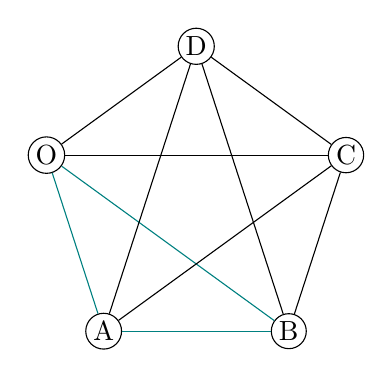
\begin{tikzpicture}
            [scale=2,
            every node/.style={circle,
            draw,
            fill=white,
            inner sep=1pt}]
            % Define positions of the 5 vertices
            \foreach \i/\name in {1/O, 2/A, 3/B, 4/C, 5/D} {
            \node (P\i) at (90+360/5*\i:1) {\name};
            }
            
            % Draw all edges of the complete graph K5
            \foreach \i in {1,...,5} {
            \foreach \j in {1,...,5} {
            \ifnum \i<\j
            \pgfmathsetmacro{\isSpecial}{
            ((\i==1 && \j==2)
            || (\i==1 && \j==3)
            || (\i==2 && \j==3))
            ? 1 : 0}
            \ifnum\isSpecial=1
            \draw[teal] (P\i) -- (P\j);
            \else
            \draw (P\i) -- (P\j);
            \fi
            \fi
            }
            }
        \end{tikzpicture}
    $$
    Since there are five points we have $v=5$. Blocks are triangles, hence $k=3$. Finally, $\lambda=3$ because given two points, any other of the three remaining points defines a new block containing the two points.

    The number of blocks is $b=\binom53=10$. The number of blocks containing a given point is $r=\binom42=6$ because we have to choose $2$ points from the remaining~$4$.

    The incidence matrix is
    $$
        A=\begin{bmatrix}
            1 & 1 & 1 & 1 & 1 & 1 & 0 & 0 & 0 & 0 \\
            1 & 1 & 1 & 0 & 0 & 0 & 1 & 1 & 1 & 0 \\ 
            1 & 0 & 0 & 1 & 1 & 0 & 1 & 0 & 0 & 1 \\
            0 & 1 & 0 & 1 & 0 & 1 & 1 & 0 & 1 & 1 \\
            0 & 0 & 1 & 0 & 1 & 1 & 0 & 1 & 1 & 1
        \end{bmatrix}
    $$
    and
    $$
        AA^T=\begin{pmatrix}
                6 & 3 & 3 & 3 & 3 \\
                3 & 6 & 3 & 3 & 3 \\
                3 & 3 & 6 & 3 & 3 \\
                3 & 3 & 3 & 6 & 3 \\
                3 & 3 & 3 & 3 & 6
            \end{pmatrix}
    $$
    with $\det(AA^T)=1458$.
\end{xmpl}

\begin{defn}
    Given a projective plane $\igeo$, a \textsl{flag} is an incident pair $(C,\block a)$ with $C \in \pts$ and $\block a \in \blocks$.\footnote{The term also applies to a sequence of incidences. It comes from the idealized image of a flagpole where the contact point on the floor is incident with the line of the pole, and the pole with the surface of the flag's fabric.}  
    Flags are sometimes written in the alternate order $(\block a,C)$.
\end{defn}


\section{Exercises}

\begin{exr}\label{exr:design-basic-combinatory}
    Given a\/ $2$-$(v,k,\lambda)$-design, determine the number of blocks containing a given point (usually denoted by\/ $r$) and the total number of blocks (usually denoted by\/ $b$).

    \textrm{\small\upshape \textbf{Gemini 2.5 Pro Hint:} Select an arbitrary point $x_0$ from the set of $v$ points. Consider the set of all flags $(y,B)$, where $B$ is a block containing $x_0$, and $y$ is a point within that same block $B$ such that $y \neq x_0$.
    The task is to determine the size of this set of flags by counting it in two distinct ways. This will lead to an equation from which $r$ can be found.}
\end{exr}

\begin{solution} Fix $O\in\pts$ and put $\pts'=\pts\setminus\set O$. Let $\blocks'$ be the set of blocks containing $O$. Consider the set of \textsl{flags}
        $$
        F = \set{(A,\block a)\in\pts'\times\blocks'\mid A\in\block a}.
        $$
        Here is a partial illustration of $F$:
    $$
        \begin{tikzpicture}[scale=0.8,
            point_node/.style={circle,
                fill=black,
                inner sep=2pt,
                draw=black}, % Style for marked points (X,x)
            axis_label/.style={font=\small},
            annotation_box/.style={draw,
                rounded corners}, % Temporarily removed opacity options
            annotationText/.style={scale=0.7,
                text centered} % Style for text within annotation boxes
            ]
            
            % Define coordinates for axis limits
                \coordinate (Origin) at (0,0);
                \coordinate (Xmax) at (4.5,0); % X-axis limit for drawing
                \coordinate (Ymax) at (0,5.5); % Y-axis limit for drawing
            
            % Draw axes
                \draw[-Stealth, thick] (Origin) -- (Xmax) node[anchor=north west] {$\mathcal{P}'$}; % X-axis for points
                \draw[-Stealth, thick] (Origin) -- (Ymax) node[anchor=south east] {$\mathcal{B}'$}; % Y-axis for blocks
            
            % Points on X-axis (elements of P')
            % Node names on the axis will be A, B, C, placed at (1,0), (2,0), (3,0)
            \foreach \xpos/\pointlabel in {1/A, 2/B, 3/C} {
                \node[axis_label, below] at (\xpos,0) (\pointlabel) {$\pointlabel$};
                \draw (\xpos,0.1) -- (\xpos,-0.1); % Tick mark
            }
            
            % Blocks on Y-axis (elements of B')
            % Node names on the axis will be blocka, blockb, blockc, blockd
            \foreach \ypos/\blocklabel/\blocknodename in {1/a/blocka, 2/b/blockb, 3/c/blockc, 4/d/blockd} {
                \node[axis_label, left] at (0,\ypos) (\blocknodename) {$\blocklabel$};
                \draw (0.1,\ypos) -- (-0.1,\ypos); % Tick mark
            }
            
            % --- Incidences based on the example scenario ---
            \node[point_node] (Aa) at (1,1) {}; % Incidence (A,a)
            \node[point_node] (Ab) at (1,2) {}; % Incidence (A,b)
            \node[point_node] (Ad) at (1,4) {}; % Incidence (A,d)
            \node[point_node] (Bc) at (2,3) {}; % Incidence (B,c)
            \node[point_node] (Cd) at (3,4) {}; % Incidence (C,d)
            
            % --- Emphasizing the details as requested ---
            
            % Detail 1: Point A is in lambda blocks from B'. (Here, lambda=3 for A)
            \draw[blue!60, loosely dashed] let \p1 = (Ymax) in (1,0) -- (1, {\y1/1pt}); % TEST 2: Draw line to where Ymax's y-value should be
            \node[draw=blue!60,
                fill=blue!10,
                annotation_box,
                annotationText,
                text width=4.8cm
            ] at (2.9,5.0)
            {Point $A \in \mathcal{P}'$ is in $\block a,\block b,\block d \in \mathcal{B}'$. \\ This illustrates that $\lambda\ge3$.};
            
            % Detail 2: A point B is in a block (e.g., B in c)
            \node[draw=green!50!black,
                fill=green!10,
                annotation_box,
                annotationText,
                text width=2.8cm] at ($(Bc)+(1.5,-0.4)$)
            {Point $B \in \mathcal{P}'$ is in block $\block c \in \mathcal{B}'$.};
            
            % Detail 3: A block d contains multiple points (e.g., A and C are in d)
            \draw[red!60, loosely dashed]
                ($(Origin |- blockd.center)+(0.0,0)$) -- ($(Xmax |- blockd.center)+(0,0)$);
            \node[draw=red!60,
                fill=red!10,
                annotation_box,
                annotationText,
                text width=3.5cm
            ] at (2.25, -1.0)
            {Block $\block d \in \mathcal{B}'$ contains points $A, C \in \mathcal{P}'$.};
        \end{tikzpicture}
    $$
    Then $r=|\blocks'|$, and since each of these blocks has $k-1$ points in $\pts'$, we deduce that $|F|=(k-1)r$.
    
    On the other hand, since there are $v-1$ points in $\pts'$, and for each of these points there are $\lambda$ blocks in $\blocks'$, we have $|F|=(v-1)\lambda$.
    
    In consequence, $(k-1)r=(v-1)\lambda$ and so
    \small
    $$
    r = \lambda\frac{v-1}{k-1}.
    $$
    \normalsize
    $\to$ In our example, $r=3(5-1)/(3-1)=6$. These are
    $$
    \blocks'=\set{ OAB, OAC, OAD, OBC, OBD, OCD}.
    $$
    
    \normalsize
    
    For the second part, consider the set of flags
    $$
        G = \set{(A,\block a)\in\pts\times\blocks\mid A\in\block a}.
    $$
    This set satisfies $|G|=bk$, where $b=|\blocks|$, because every block has $k$ points.

    On the other hand $|G|=vr$, since every point belongs to precisely $r$ blocks. It follows that
    $$
        b=\frac{vr}{k} = \lambda\frac{v^2-v}{k^2-k}.
    $$
\end{solution}

\begin{exr}\label{exr:design-projective-plane}
    Show that a\/ $2$-$(n^2+n+1, n+1, 1)$ design is a projective plane if\/ $n \geq 2$. (Note that this can be regarded as an alternative definition of finite projective planes.)
\end{exr}

\begin{solution}
    Since $\lambda=1$, axiom~\PP1 is automatically met.
    
    For axiom~\PP2, suppose, for a contradiction, that $\block a\ne\block b\in\blocks$, don't satisfy it. There are two cases (i)~$\block a\cap\block b=\emptyset$ and (ii)~$A\ne B\in\block a\cap\block b$.

    In case (i) let $\block a=\set{A_1,\dots,A_k}$ and $\block b=\set{B_1,\dots,B_k}$. The blocks $A_iB_j$ are distinct. Indeed, if $\block c=A_iB_j=A_{i'}B_{j'}$ with $j\ne j'$, then $\block c=B_jB_{j'}=\block b$ and $A_i\in\block b$, which is not the case. Thus $\block c=A_iB_j=A_{i'}B_j$ and the same argument shows that $i=i'$. This shows that there are at least $k^2+2$ blocks in the design, i.e.,
    \begin{align*}
        n^2+2n+3 &= k^2+2\\
            &\le b\\
            &= \lambda\frac{v(v-1)}{k(k-1)}\\
            &=\frac{(n^2+n+1)(n^2+n)}{(n+1)n}\\
            &= n^2+n+1,
    \end{align*}
    which is impossible.

    Case (ii) is also impossible because it violates~\PP1.

    To complete the proof, it suffices to show condition P3' from Lemma~\ref{lem:alternative-projective-axiom}, namely that given two lines $\block a\ne\block b$, there is always a point not incident with either of them. Suppose the contrary. Then we would have $v=2k-1$, which is impossible when $n\ge2$ because it translates into $n^2+n+1=2(n+1)-1$ or $n(n-1)=0$. Since the order $n$ is assumed to be at least $2$, this is a contradiction.

\end{solution}

\begin{test}
    From Example~\ref{xmpl:triangular-design}, we have $r=6$ and $b=10$, which agree with
    \begin{align*}
        \lambda\frac{v-1}{k-1}&=3\frac42=6
        \intertext{and}
        \lambda\frac{v(v-1)}{k(k-1)}&=3\frac{5\cdot4}{3\cdot2}
            =10.
    \end{align*}
\end{test}

\begin{exr}\label{exr:design-affine-plane}
    Show that a\/ $2$-$(n^2, n, 1)$ design is an affine plane if\/ $n \geq 2$.
\end{exr}

\begin{solution}
    Since $\lambda=1$, axiom~\ref{A1} is automatically met.

    Firstly observe that, by Exercise~\ref{exr:design-basic-combinatory}, the number of blocks is
    $$
        b=\lambda\frac{v-1}{k-1}=\frac{n^2-1}{n-1}=n+1.
    $$
    Now consider a point $A$ and a block $\block a$ with $A\notin\block a$. Suppose that axiom~\ref{A2} doesn't hold. There are two possibilities: (i)~every block passing through $A$ intersects $\block a$, or (ii)~there are (at least) two distinct lines that don't intersect~$\block a$ and pass through~$A$.

    In (i) we would have $n$ blocks passing through $A$. Hence,
    $$
        n=b=n+1\quad\noend
    $$
    In (ii) we would have at least $n+2$ blocks passing through $A$, i.e.,
    $$
        n+2\le b=n+1\quad\noend
    $$
    Axiom~\ref{A3} is given.

    Axiom~\ref{A4} is clear since, as we saw above, the number $r$ of incident blocks with a point is $n+1$.
    
\end{solution}


\begin{exr}
    Consider the defining axioms for projective planes and the numerical properties in\/ {\upshape Theorem~\ref{thm:order-is-well-defined}}. Try to find other possible sets of axioms for projective planes. Do the same for affine planes.
\end{exr}

\begin{solution}
    Suppose that $\Pi=\igeo$ is an incidence geometry satisfying
   \begin{enumerate}[q$_1$,font=\upshape\scshape]
        \item Every pair of distinct points is incident with exactly one block.
        \item Every block of\/ $\Pi$ is incident with\/ $n+1$ points.
        \item Every point of\/ $\Pi$ is incident with\/ $n+1$ blocks.
    \end{enumerate}
    Conditions \textsc{q$_1$} and \textsc{q$_2$} imply that $\Pi$ is a $2$-$(v,n+1,1)$ design. Thus, according to Exercise~\ref{exr:design-basic-combinatory},
    $$
        r=\frac{v-1}n.
    $$
    Since $r=n+1$ by \textsc{q$_3$}, we have $v=n^2+n+1$. Then $\Pi$ is a $2$-$(n^2+n+1,n+1,1)$ design, hence a projective plane by Exercise~\ref{exr:design-projective-plane}, provided that $n\ge2$.

    For the affine plane suppose that $n\ge2$ and consider
    \begin{enumerate}[b$_1$,font=\upshape\scshape]
        \item Every pair of distinct points is incident with exactly one block.
        \item Every block of\/ $\Pi$ is incident with\/ $n$ points.
        \item Every point of\/ $\Pi$ is incident with\/ $n+1$ blocks.
    \end{enumerate}
    Conditions \textsc{b$_1$} and \textsc{b$_2$} imply that $\Pi$ is a $2$-$(v,n,1)$ design. Thus, according to Exercise~\ref{exr:design-basic-combinatory},
    $$
        r=\frac{v-1}{n-1}.
    $$
    Since $r=n+1$ by \textsc{b$_3$}, we have $v=n^2$. Then $\Pi$ is a $2$-$(n^2,n,1)$ design, hence a projective plane by Exercise~\ref{exr:design-affine-plane}, provided that $n\ge2$.

\end{solution}

\begin{exr}\label{exr:design-incidence-matrix}
    Determine\/ $AA^T$ for an incidence matrix of a\/ $2$-$(v,k,\lambda)$ design.
\end{exr}

\begin{solution}
   Let $\set{\block a_1,\dots,\block a_b}$ be the set of blocks and $\set{A_1,\dots,A_v}$ the set of points. Let $A$ be the $b\times v$ incidence matrix of the design, where rows represent blocks and columns points, i.e.,
    $$
        a_{ij} = \ev A(i,j) = \begin{cases}
            1
                &\text{if the $i$th block is incident with the $j$th point},\\
            0   &\text{otherwise}.
        \end{cases}
    $$
    Therefore,
    \begin{equation}\label{eq:AA^T}
        \ev{AA^T}(i,j) = \sum_{h=1}^va_{ih}a_{jh}
            = \begin{cases}
                k   &\text{if }i=j,\\
                |\block a_i\cap\block a_j|
                    &\text{if }i\ne j.
            \end{cases}
    \end{equation}
    On the other hand, the entries of $A^T$ satisfy
    \[
        \ev{A^T}(i,j) = a_{ji}
            \begin{cases}
            1
                &\text{if }A_i\in\block a_j,\\
            0   &\text{otherwise}.
        \end{cases}
    \]
    The product $A^T\!A$ is then the square matrix whose $(i,j)$th entry is
    \[
        \ev{A^T\!A}(i,j) = \sum_{h=1}^b a_{hi} a_{hj},
    \]
    which counts the number of blocks $\block a_h$ incident with $A_i$ and $A_j$. Hence,
    \begin{equation}\label{eq:A^TA}
        \ev{A^T\!A}(i,j) = 
            \begin{cases}
                r & \text{if } i=j,\\
                \lambda   & \text{if } i\ne j,
            \end{cases}
    \end{equation}
    where $r=\lambda\dfrac{v-1}{k-1}$. It follows that $A^T\!A = \lambda U + (r-\lambda)I$.
\end{solution}

\begin{exr}
    Show that for\/ $k < v$ one has\/ $b \geq v$ for a\/ $2$-$(v,k,\lambda)$ design.
    
    \textrm{\upshape Hint: use the matrix\/ $A^T\!A$.}
\end{exr}

\begin{solution}
    By the previous exercise, we have
    \begin{align*}
       \det(A^T\!A) &= \det\begin{bmatrix}
                r& \lambda & \cdots & \lambda \\
                \lambda & r & \cdots & \lambda \\
                \vdots & \vdots & \ddots & \vdots \\
                \lambda & \lambda & \cdots & r
            \end{bmatrix},
        \intertext{subtracting first column from any other column:}
            &= \det \begin{bmatrix}
                r & \lambda-r & \lambda - r & \cdots & \lambda - r \\
                \lambda & r - \lambda & 0 & \cdots & 0 \\
                \lambda & 0 & r - \lambda & \cdots & 0 \\
                \vdots & \vdots & \vdots & \ddots & \vdots \\
                \lambda & 0 & 0 & \cdots & r - \lambda
            \end{bmatrix},
        \intertext{adding to the first row all other rows:}
            &= \det \begin{bmatrix}
                r+(v-1)\lambda & 0 & 0 & \cdots & 0 \\
                \lambda & r - \lambda & 0 & \cdots & 0 \\
                \lambda & 0 & r - \lambda & \cdots & 0 \\
                \vdots & \vdots & \vdots & \ddots & \vdots \\
                \lambda & 0 & 0 & \cdots & r - \lambda
            \end{bmatrix}\\
            &= (r+(v-1)\lambda)(r-\lambda)^{v-1}.
        \end{align*}
        Since
        \begin{align*}
            r-\lambda=0
                \iff \bcancel\lambda\frac{v-1}{k-1}=\bcancel\lambda
                \iff v=k\quad\noend
        \end{align*}
        we deduce that $A^T\!A$ is nonsingular. In particular, the linear map $\Q^v\to\Q^b$, $\vect x\mapsto A\vect x$, is injective. But this can only happen if $b\ge v$.

\end{solution}

\begin{test}
    In the case of a projective plane the computation above yields to
    $$
        (r+(v-1)\lambda)(r-\lambda)^{v-1}=(n+1+n^2+n)n^{n^2+n},
    $$
    which agrees with Lemma~\ref{lem:characteristic-polynomial-AA^T-projective-plane} in that $\det(AA^T)=(n+1)^2n^{n^2+n}$.
\end{test}

\begin{test}
    According to Example~\ref{xmpl:triangular-design}, $\det(AA^T)=1458$ and $r=6$. Coincidentally,
    $$
        (r+(v-1)\lambda)(r-\lambda)^{v-1}
            = (6+4\cdot3)(6-3)^4=18\cdot81=1458.
    $$
\end{test}

\begin{exr}
     Prove that any finite projective plane of order at least\/ $3$ contains a (closed)\footnote{The term \textit{closed} emphasizes that the Desargues theorem holds true for a specific arrangement of ten points and ten lines.} Desargues configuration.
\end{exr}

\begin{solution}
    See Theorem \ref{thm:ostrom}.
\end{solution}
    

\begin{exr}\label{exr:order-4=PG(2,4)}
    Show that there is a unique projective plane of order\/~$4$ and\/~$5$.
\end{exr}

\begin{solution}
    \begin{description}
        \item[Order $4$.] In this case, there is a total of $4^2+4+1=21$ points, with lines containing $5$ points, and with every point incident with $5$ lines.

        %\if{false}
        By Remark~\ref{rem:order-of-galois-plane}, we know that the Galois plane $\PG(2,2^2)$ has order $4$. Therefore, we need to show that any other plane of order $4$ is isomorphic to it.

        Let $\Fq[2^2]=\set{0,1,i,i^2}$, where $i^2=i+1$. The addition and multiplication tables are
        $$
        \begin{array}{l|llll}
             +&0&1&i&i^2 \\
             \hline\rule{0pt}{11pt}
             0&0&1&i&i^2\\
             1&1&0&i^2&i\\
             i&i&i^2&0&1\\
             i^2&i^2&i&1&0
        \end{array}
        \qquad
        \begin{array}{l|llll}
             \cdot&0&1&i&i^2 \\
             \hline\rule{0pt}{11pt}
             0&0&0&0&0\\
             1&0&1&i&i^2\\
             i&0&i&i^2&1\\
             i^2&0&i^2&1&i
        \end{array}        
        $$
        Let $\Pi=\igeo$ be a projective plane of order~$4$. Take a line $\ell$ and remove it from $\Pi$ to obtain an affine plane $\Lambda$ of order $4$. Select two points $X\ne Y$ of $\ell$, and consider their parallel pencils in $\Lambda$. Since each pencil has $4$ (affine) points, we will identify them using the four elements of $\Fq[2^2]$, namely $(\block x_0,\block x_1,\block x_i,\block x_{i^2})$ and $(\block y_0,\block y_1,\block y_i,\block y_{i^2})$. Define
        \begin{align*}
            f\colon\Fq[2^2]\times\Fq[2^2]&\to\pts\setminus\tr(\ell)\\
            (a,b)&\mapsto\block x_a\wedge\block y_b
        \end{align*}
        which is well-defined because these two pencils don't intersect at $\tr(\ell)$.
        
        Since $|\dom(f)|=16=|\pts\setminus\tr(\ell)|$, to see that $f$ is a bijection, it suffices to show that it is injective. Suppose that $\block x_a \wedge \block y_b = \block x_{a'} \wedge \block y_{b'}$, and let~$C$ denote this point. Then $C \in \tr(\block x_a)\cap\tr(\block x_{a'})$, which forces $a = a'$, since otherwise $\block x_a \parallel \block x_{a'}$. A similar argument shows that $b=b'$.
        
        Let $\mathcal L$ denote the set of lines in $\AG(2,2^2)$. Each element of $\mathcal L$ is defined by the point with homogeneous coordinates $(a:b:c)$, which we will identify with a linear equation of which we have two types: $y=ax+b$ and $x=c$. Introduce
        \begin{align*}
            \varphi\colon\mathcal L&\to\blocks\setminus\set\ell\\
            y=ax+b&\mapsto (\block x_0\wedge\block y_b)
                (\block x_1\wedge\block y_{a+b})\\
            x=c&\mapsto\block x_c,
        \end{align*}
        which is well-defined since the injectivity of $f$ implies
        $$
            \block x_0\wedge\block y_b=f(0,b)
                \ne f(1,a+b)=\block x_1\wedge\block y_{a+b}.
        $$
        Let $\block z=\varphi(y=ax+b)=(\block x_0\wedge\block y_b)(\block x_1\wedge\block y_{a+b})$. In what follows we will use this notation.

        \needspace{2\baselineskip}
        \textbf{Claim 1.} \textit{There are two possibilities for\/ $\tr(\block z)$. These are:}
        \begin{enumerate}[(1)]
            \item $\tr(\block z) = \set{\block x_0\wedge\block y_b,\;
                \block x_1\wedge\block y_{a+b},\;
                \block x_i\wedge\block y_{ai+b},\;
                \block x_{i^2}\wedge\block y_{ai^2+b}}$,
                \label{eq:tr(z)} or
            \item $\tr(\block z) = \set{\block x_0\wedge\block y_b,\;
                \block x_1\wedge\block y_{a+b},\;
                \block x_i\wedge\block y_{ai^2+b},\;
                \block x_{i^2}\wedge\block y_{ai+b}}$.
                \label{eq:tr(z)-twisted}
        \end{enumerate}
        
        Since every (affine) line has $4$ points, and the injectivity of the function~$f$ ensures that both sets above have size $4$, the claim holds if either $\block x_i\wedge\block y_{ai+b}$ or $\block x_i\wedge\block y_{ai^2+b}$ lies on $\block z$.
            
        The case $a = 0$ is immediate, since in that case $\block z = \block y_b$.
        
        For $a \ne 0$, the map $x \mapsto ax + b$ is a bijection. Thus, if $\block x_i\wedge\block y_z$ lies on~$\block z$, the only admissible values for $z$ are $z = ai + b$ or $z = ai^2 + b$. To see this, we must exclude the values $z = a\cdot 0 + b$ and $z = a\cdot 1 + b$. The first case implies
        \[
            \block z = (\block x_0\wedge\block y_b)(\block x_i\wedge\block y_b) = \block y_b,
        \]
        which can only occur if $a = 0$. The second case implies
        \[
            \block z = (\block x_1\wedge\block y_{a+b})(\block x_i\wedge\block y_{a+b}) = \block y_{a+b}.
        \]
        But since $\block x_0\wedge\block y_b \in \block z$, this would force $\block y_b$ and $\block y_{a+b}$ to intersect in $\Lambda$, which is impossible when $a \ne 0$. 

        \medskip

        \textbf{Claim 2.} \textit{Equation\/ {\upshape\ref{eq:tr(z)-twisted}} does not hold when\/ $a\ne0$.}

        By definition $\block z=(\block x_0\wedge\block y_b)(\block x_1\wedge\block y_{a+b})$. Let $Z=\ell\wedge\block z$ be the point at infinity associated with~$\block z$. Then $Z\ne X$ because equality would imply that $\block z\parallel\block x_0$, which is impossible because $\block z$ is incident with an affine point on~$\block x_0$ (as well as another on~$\block x_1$). Similarly, $Z\ne Y$.

        Suppose that equation~\ref{eq:tr(z)} is not true. By Claim~1 equation~\ref{eq:tr(z)-twisted} must hold. Therefore, $\ell\wedge(\block x_0\wedge\block y_b)(\block x_i\wedge\block y_{ai^2+b})=Z$.
        
        Then $\block z\ne(\block x_0\wedge\block y_b)(\block x_i\wedge\block y_{ai+b})$, since otherwise the only possibility for ${\block x_{i^2}}\wedge\block z$ would be $\block x_{i^2}\wedge\block y_{ai^2+b}$, implying equation~\ref{eq:tr(z)}. Thus, this line intersects $\ell$ at a point $P\ne X,Y,Z$. Similarly, $(\block x_0\wedge\block y_b)(\block x_{i^2}\wedge\block y_{ai^2+b})$ intersects $\ell$ at a point $Q\ne X,Y,Z$.

        If $P=Q$, then the line $(\block x_0\wedge\block y_b)(\block x_i\wedge\block y_{ai+b})=(\block x_0\wedge\block y_b)(\block x_{i^2}\wedge\block y_{ai^2+b})$ would intersect $\block x_1$ at $\block x_1\wedge\block y_{a+b}$ (since no other $\block y_*$ is available). This, however, would force $\block x_1\wedge\block y_{a+b}$ to be collinear with the other three points, which contradicts our original premise. Consequently, 
        $P\ne Q$, and we deduce that $\tr(\ell)=\set{X,Y,Z,P,Q}$.
        
        Put $R=\ell\wedge(\block x_i\wedge\block y_{ai+b})(\block x_{i^2}\wedge\block y_{ai^2+b})$. Clearly, $R\ne X,Y$. In addition, $R\ne Z$ by equation~\ref{eq:tr(z)-twisted}. It follows that $R=P$ or $R=Q$. But
        \begin{align*}
            R=P&\implies
                (\block x_i\wedge\block y_{ai+b})
                    (\block x_{i^2}\wedge\block y_{ai^2+b})
                    =(\block x_0\wedge\block y_b)
                    (\block x_i\wedge\block y_{ai+b})\\
                &\implies\set{\block x_0\wedge\block y_b,\;
                    \block x_i\wedge\block y_{ai+b},\;
                    \block x_{i^2}\wedge\block y_{ai^2+b}}
                    \text{ is collinear}\\
                &\implies \text{equation \ref{eq:tr(z)} holds true} 
                    \noend\\
            R=Q&\implies
                (\block x_i\wedge\block y_{ai+b})
                    (\block x_{i^2}\wedge\block y_{ai^2+b})
                    =(\block x_0\wedge\block y_b)
                    (\block x_{i^2}\wedge\block y_{ai^2+b})\\
                &\implies\set{\block x_0\wedge\block y_b,\;
                    \block x_i\wedge\block y_{ai+b},\;
                    \block x_{i^2}\wedge\block y_{ai^2+b}}
                    \text{ is collinear}\\
                &\implies \text{equation \ref{eq:tr(z)} holds true} 
                    \noend
        \end{align*}
        Claim 2 is now proved. 

        \medskip

        \textbf{Claim 3.} \textit{$\varphi$ is bijective.}
        
        It suffices to show that $\varphi$ is injective (domain and codomain are of equal size). To verify this, first observe that $\varphi(y=ax+b)\ne\varphi(x=c)$. Indeed, otherwise $\block x_0\wedge\block y_b\in\block x_0\cap\block x_c$, which implies $c=0$. Similarly, we would have $c=1$, which is a contradiction. 

        Now suppose that $\varphi(y=ax+b)=\varphi(y=a'x+b')$. Since $\block x_0 \parallel \block x_1, \block x_i, \block x_{i^2}$, the only way for the point $\block x_0 \wedge \block y_{b'}$ to lie on~$\block z$ is for it to coincide with $\block x_0 \wedge \block y_b$. This forces $\block y_b = \block y_{b'}$, i.e., $b = b'$, since otherwise the lines $\block y_b$ and $\block y_{b'}$ would be disjoint.

        From the equality $b' = b$ it follows that $\block x_1\wedge\block y_{a'+b}$ lies on $\block z$. Once again, the only possibility for this to happen is that
        \[
        \block x_1\wedge\block y_{a'+b} = \block x_1\wedge\block y_{a+b}.
        \]
        This forces $\block y_{a'+b} = \block y_{a+b}$, since otherwise the lines $\block y_{a'+b}$ and $\block y_{a+b}$ would intersect, which is impossible. Consequently, $a = a'$.
        
        Finally, $\block x_c = \block x_{c'}$ implies $c = c'$. The injectivity of $\varphi$ is now established.

        \medskip

        \textbf{Conclusion.} The pair $(f,\varphi)$ is an isomorphism between $\AG(2,2^2)$ and~$\Lambda$. This isomorphism can be extended to an isomorphism between $\PG(2,2^2)$ and~$\Pi$ by mapping
        \begin{align*}
            [a:b:0]\xmapsto f
                (\block x_0\wedge\block y_0)
                (\block x_a\wedge\block y_b)\wedge\ell,
                \quad
            z=0\xmapsto\varphi\ell.
        \end{align*}
        %\fi

        \needspace{3\baselineskip}
        Below we include another solution that follows a different approach.
        
        \textbf{Construction.} \citep{cuypers} Let $\Pi$ be a projective plane of order $4$. Take four points $\set{A_1,A_2,A_3,A_4}$ in general position. Consider the lines $\block a_{ij}=A_iA_j$, for $1\le i<j\le4$.
        $$
            \begin{tikzpicture}[
                scale=0.6,
                font=\small, % Sets default font to \small for nodes and labels
                point/.style={circle, fill=black, inner sep=1.2pt, draw=black},
                line/.style={thin}
                ]
                
                % Define coordinates for the 4 points in general position
                % (Chosen to form a convex quadrangle for clarity)
                \coordinate (coord_A1) at (0,0);
                \coordinate (coord_A2) at (3.5,0.5);
                \coordinate (coord_A3) at (4.5,2.7);
                \coordinate (coord_A4) at (0.5,3.2);
                
                % Draw and label the points
                % Node names are A1, A2, A3, A4 for easy reference
                \node[point, label={below right:$A_1$}]  (A1) at (coord_A1) {};
                \node[point, label={[xshift=2pt]below:$A_2$}] (A2) at (coord_A2) {};
                \node[point, label={above left:$A_3$}] (A3) at (coord_A3) {};
                \node[point, label={above right:$A_4$}]  (A4) at (coord_A4) {};
                
                % Draw the 6 lines a_ij = A_i A_j, extending them slightly
                % You can replace $a_{ij}$ with $\block{a}_{ij}$ if your \block command is defined
                % The 'auto' option tries to place the label conveniently, 'sloped' aligns it with the line.
                % 'swap' can be used with 'auto' to flip the label to the other side if needed.
                
                % Line a_12 (A1-A2)
                \draw[line,name path=a12] ($(A1)!-1cm!(A2)$) -- ($(A2)!-1cm!(A1)$) node[midway, auto, sloped, below] {$\block a_{12}$};
                
                % Line a_13 (A1-A3)
                \draw[line,name path=a13] ($(A1)!-0.8cm!(A3)$) -- ($(A3)!-0.8cm!(A1)$) node[right, auto, sloped] {$\block a_{13}$};
                
                % Line a_14 (A1-A4)
                \draw[line,name path=a14] ($(A1)!-0.8cm!(A4)$) -- ($(A4)!-0.8cm!(A1)$) node[midway, auto, sloped] {$\block a_{14}$};
                
                % Line a_23 (A2-A3)
                \draw[line,name path=a23] ($(A2)!-0.8cm!(A3)$) -- ($(A3)!-0.8cm!(A2)$) node[midway, auto, sloped, swap] {$\block a_{23}$};
                
                % Line a_24 (A2-A4)
                \draw[line,name path=a24] ($(A2)!-1cm!(A4)$) -- ($(A4)!-1cm!(A2)$) node[left, auto, sloped] {$\block a_{24}$};
                
                % Line a_34 (A3-A4)
                \draw[line,name path=a34] ($(A3)!-1cm!(A4)$) -- ($(A4)!-1cm!(A3)$) node[midway, auto, sloped, above] {$\block a_{34}$};

                % D1
                \path[name intersections={of=a24 and a13, by= D1}];
                \node[point, label={below:$\block D_1$}] at (D1) {};
            \end{tikzpicture}
        $$
        Introduce the \textsl{diagonal} points (of which only $D_1$ is shown in the picture)
        {\small\begin{align*}
            D_1 &= \block a_{13}\wedge\block a_{24},
            &D_2 &= \block a_{12}\wedge\block a_{34},
            &D_3 &= \block a_{14}\wedge\block a_{23}.
        \end{align*}}

        \vspace{-0.3\baselineskip}
        \needspace{2\baselineskip}
        \textbf{Claim 1.} \textit{The three diagonal points are aligned.}
        \begin{quote}
            Suppose, for the sake of contradiction, that $D_3$ is not incident with $\ell=D_1D_2$. Take $X\in\ell\setminus\set{D_1,D_2}$. Then $X\notin\block a_{13}\cup\block a_{24}$. Therefore, from the six lines under consideration, $X$ could only be in $\block a_{14}$ or $\block a_{23}$, not in both. Since there are $5=4+1$ points in $\ell$, there are three possibilities for $X$. Hence, one of them is not incident with any of the six lines.

            A similar argument applied to $D_1D_3$ and $D_2D_3$ shows that there are, at least, two other points in addition to the ones in the six lines, one in $D_1D_3$ and the other in $D_2D_3$. Since there are $6\times 2=12$ unnamed points in the six lines of the quadrilateral, and the named ones are $7$, we would have $12+7+3=22$ distinct points in $\Pi$, which is impossible. The claim is now clear.
        \end{quote}
        
        Let $\block d$ be the line through $D_1$, $D_2$ and $D_3$ and let $A_5$ and $A_6$ be such that $\block d=\set{D_1,D_2,D_3,A_5,A_6}$.

        \textbf{Claim 2.} \textit{The points of\/ $\mathcal O=\set{A_1,\dots,A_6}$ are in general position.}

        \begin{quote}
            By construction, $A_1, \dots, A_4$ are in general position. Moreover, if any two of these points—say, $A_1$ and $A_2$—were collinear with either $A_5$ or $A_6$, then $\block d$ would coincide with $\block a_{12}$, which is not the case. Similarly, if $A_5$ and $A_6$ were collinear with, say $A_1$, then $A_1$ would lie on $\block d$, which is also impossible.
        \end{quote}

        \needspace{2\baselineskip}
        \textbf{Claim 3.} \textit{Each line in\/ $\Pi$ meets $\mathcal O$ in\/ $0$ or\/ $2$ points.}

        \begin{quote}
            By Claim~1 it is enough to see that no line intersects $\mathcal O$ in exactly $1$ point (i.e., $\mathcal O$ has no tangents). Suppose otherwise. Let $\block t$ be a tangent to $\mathcal O$ at $A_i$. There are two cases: (a)~$i\in\set{1,2,3,4}$, or (b)~$i\in\set{5,6}$.
            
            In (a) we may assume, without loss of generality, that $A_1\in\block t$. If $\block t\wedge\block d\in\set{D_1,D_2,D_3}$, then $\block t=A_1D_j$, which is incident with another $D_k$. Hence $\block t=\block d$, which contains $A_5$ and $A_6$. Thus, $\block t\wedge\block d\notin\set{D_1,D_2,D_3}$, which implies that  $\block t$ is incident with $A_5$ or $A_6$, which is a contradiction because $A_1\in\block t$.

            In (b) $A_i\in\block t$. But this is impossible because $A_iA_1,\dots, A_iA_4$, and $\block d$ exhaust the $4+1$ lines through~$A_i$, and $\block t$ is not one of them.
        \end{quote}

        \textbf{Note.} A set of $6$ points that satisfies Claims~2 and~3 is called a \textsl{hyperoval}.

        \textbf{Claim 4.} \textit{$\mathcal O$ is the only hyperoval including\/ $\set{A_1,A_2,A_3,A_4}$.}

        \begin{quote}
            Suppose that $\mathcal Q=\set{A_1,A_2,A_3,A_4,B_5,B_6}$ satisfies Claims~2 and~3. 

            So far, we have established that there are $6\times 2$ unnamed points, plus $7+2$ already named. This gives the total of $21$ points in~$\Pi$, which locks the possibilities for $B_5$ and $B_6$. Firstly observe that $B_i$ cannot be one of the $12$ named points because that would mean that $\mathcal Q$ is not in general position. Since $B_i\notin\set{A_1,\dots,A_4}$, there are two options: (a)~$B_i\in\set{D_1,D_2,D_3}$, or (b)~$B_i\in\set{A_5,A_6}$. We can discard (a) because, in that case, $B_i$ would be collinear with two points of $\set{A_1,\dots,A_4}$. As a result, $B_i\in\set{A_5,A_6}$, as claimed.
        \end{quote}
        There are\/ $21 - 6 = 15$\/ points in\/ $\Pi$ external to~$\mathcal O$. Let\/ $R$ be one of them. From the pencil of\/ $5$\/ lines through\/ $R$, exactly\/ $3$\/ intersect\/ $\mathcal O$, since any such line must be secant—i.e., it intersects\/ $\mathcal O$\/ in two points. These three secant lines determine a partition of $\mathcal O$ into $3$ sets of $2$ points each. The total number of partitions into $3$ sets of $2$ points is
        \begin{equation}\label{eq:15-patitions}
            \#\mathrm{partitions}=\frac{\binom62\binom42\binom22}{3!}
                = \frac{(3\cdot5)(6)(1)}{6}
                = 15.
        \end{equation}
        Therefore, there is a bijective correspondence between the points external to $\mathcal O$ and said partitions.

        Each of these partitions can be visualized as a set of~$3$ disjoint edges in the complete graph $K_6$ of six nodes, as illustrated in the example below
        $$
            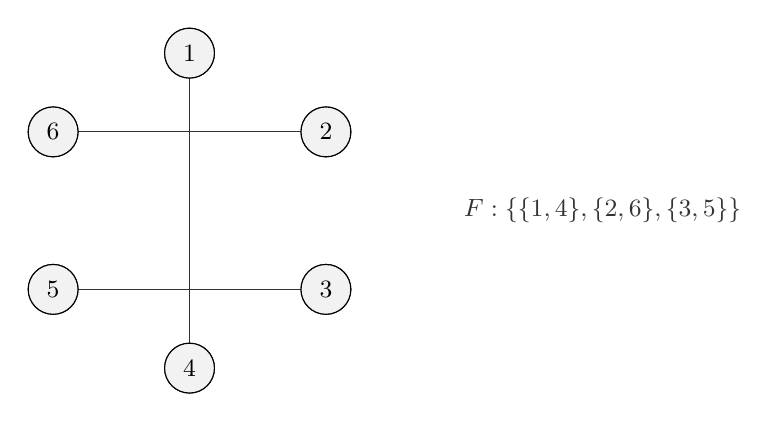
\begin{tikzpicture}[
                scale=0.8,
                vertex/.style={circle, draw, fill=gray!10, inner sep=2pt, minimum size=18pt},
                edge/.style={thin}
                ]
            
                % Define radius for vertex placement
                \def\radius{2.5cm}
                
                % Define the vertices
                \foreach \i in {1,...,6} {
                    \coordinate (v\i) at ({90 - (\i-1)*60}:\radius);
                    \node[vertex] at (v\i) {\i};
                }
                
                % Define colors for each matching
                % These are standard TikZ/xcolor names.
                \colorlet{colorF}{white!20!black} % A darker green
                
                % Draw edges for F = {(1,4), (2,6), (3,5)}
                \foreach \u/\v in {1/4, 2/6, 3/5} {
                    \draw[colorF, edge] (v\u) -- (v\v);
                }
                                
                % Add a legend
                \begin{scope}[xshift=\radius+1.2cm, yshift=1.2cm, font=\small] % Adjust xshift/yshift to position legend
        
                    \node[anchor=west, color=colorF] at (0.5, -1.2) {$F: \{\{1,4\},\{2,6\},\{3,5\}\}$};
                    \draw[white, edge] (0,-1.2) -- (0.4,-1.2);
                
                    % Draw the vertices
                    \foreach \i in {1,...,6} {
                        \node[vertex] at (v\i) {\i};
                    }
                \end{scope}
            
            \end{tikzpicture}
        $$
        In the language of graphs, these partitions are called \textsl{$1$-factors}. In addition, a \textsl{$1$-factorization} of\/ $K_6$ is a collection of\/ $1$-factors, pairwise edge-disjoint, whose union covers all edges of the graph. Since\/ $K_6$ has\/ $\binom62=15$ edges, a\/ $1$-factorization consists of\/ $5$\/ $1$-factors.

        $$
            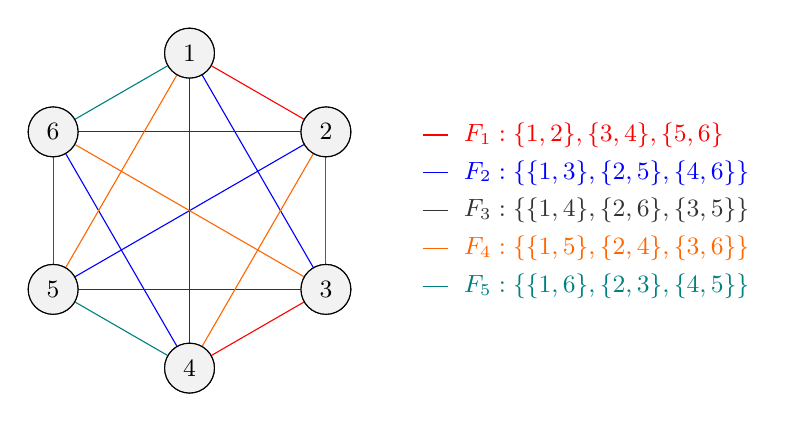
\begin{tikzpicture}[
                scale=0.8,
                vertex/.style={circle, draw, fill=gray!10, inner sep=2pt, minimum size=18pt},
                edge/.style={thin}]
            
                % Define radius for vertex placement
                \def\radius{2.5cm}
                
                % Define the vertices
                \foreach \i in {1,...,6} {
                    \coordinate (v\i) at ({90 - (\i-1)*60}:\radius);
                    \node[vertex] at (v\i) {\i};
                }
                
                % Define colors for each matching
                % These are standard TikZ/xcolor names.
                \colorlet{colorF1}{red}
                \colorlet{colorF2}{blue}
                \colorlet{colorF3}{white!20!black} % A darker green
                \colorlet{colorF4}{orange!80!red}
                \colorlet{colorF5}{teal}
                
                % Draw edges for F1 = {(1,2), (3,4), (5,6)}
                \foreach \u/\v in {1/2, 3/4, 5/6} {
                    \draw[colorF1, edge] (v\u) -- (v\v);
                }
                
                % Draw edges for F2 = {(1,3), (2,5), (4,6)}
                \foreach \u/\v in {1/3, 2/5, 4/6} {
                    \draw[colorF2, edge] (v\u) -- (v\v);
                }
                
                % Draw edges for F3 = {(1,4), (2,6), (3,5)}
                \foreach \u/\v in {1/4, 2/6, 3/5} {
                    \draw[colorF3, edge] (v\u) -- (v\v);
                }
                
                % Draw edges for F4 = {(1,5), (2,4), (3,6)}
                \foreach \u/\v in {1/5, 2/4, 3/6} {
                    \draw[colorF4, edge] (v\u) -- (v\v);
                }
                
                % Draw edges for F5 = {(1,6), (2,3), (4,5)}
                \foreach \u/\v in {1/6, 2/3, 4/5} {
                    \draw[colorF5, edge] (v\u) -- (v\v);
                }
                
                % Add a legend
                \begin{scope}[xshift=\radius+1.2cm, yshift=1.2cm, font=\small] % Adjust xshift/yshift to position legend
                    \node[anchor=west, color=colorF1] at (0.5, 0) {$F_1: \set{\{1,2\},\{3,4\},\{5,6\}}$};
                    \draw[colorF1, edge] (0,0) -- (0.4,0);
                
                    \node[anchor=west, color=colorF2] at (0.5, -0.6) {$F_2: \{\{1,3\},\{2,5\},\{4,6\}\}$};
                    \draw[colorF2, edge] (0,-0.6) -- (0.4,-0.6);
                
                    \node[anchor=west, color=colorF3] at (0.5, -1.2) {$F_3: \{\{1,4\},\{2,6\},\{3,5\}\}$};
                    \draw[colorF3, edge] (0,-1.2) -- (0.4,-1.2);
                
                    \node[anchor=west, color=colorF4] at (0.5, -1.8) {$F_4: \{\{1,5\},\{2,4\},\{3,6\}\}$};
                    \draw[colorF4, edge] (0,-1.8) -- (0.4,-1.8);
                
                    \node[anchor=west, color=colorF5] at (0.5, -2.4) {$F_5: \{\{1,6\},\{2,3\},\{4,5\}\}$};
                    \draw[colorF5, edge] (0,-2.4) -- (0.4,-2.4);
                
                    % Draw the vertices
                    \foreach \i in {1,...,6} {
                        \node[vertex] at (v\i) {\i};
                    }
                \end{scope}
            
            \end{tikzpicture}
        $$
        \textbf{Note.} A subgraph of $K_6$ is \textsl{$2$-regular} if each node has degree~$2$.
        
        \textbf{Claim 4.} \textit{If\/ $F$ and\/ $G$ are edge-disjoint\/ $1$-factors, then\/ $F\cup G$ is\/ $2$-regular with one edge in\/~$F$ and the other in\/~$G$ at every node.}

        \begin{quote}
            After renaming the nodes, we may assume that
            \begin{align*}
                F &= \{\{1,2\},\{3,4\},\{5,6\}\}\\
                G &= \{\{1,n_1\},\{2,n_2\},\{n_3,n_4\}\}
            \end{align*}
            Since $n_1\ne2$, we see that the node labeled $1$ has degree $2$, with an edge in $F$, namely $\{1,2\}$, and the other in $G$, $\{1,n_1\}$. Since this node is representative of all others (modulo rename), the conclusion is clear.            
        \end{quote}

        \needspace{3\baselineskip}
        \textbf{Claim 5.} \textit{The union of two edge-disjoint\/ $1$-factors is a simple cycle of order\/~$6$.}

        \begin{quote}
            This is a direct consequence of Claim~4 because it implies that $F\cup G$ has $3+3=6$ edges that alternate to visit all nodes. Further renaming node $n_2$ to be $3$, we have
             \begin{align*}
                F &= \{\{1,2\},\{3,4\},\{5,6\}\}\\
                G &= \{\{1,n_1\},\{2,3\},\{n_3,n_4\}\}
            \end{align*}
            we are left with two possibilities for the $G$-edge at $4$: $n_1$ or $n_3$. However, such an edge cannot be $\{1,n_1\}$ because that would mean $n_1=4$ and, \textit{a fortiori}, $\{n_3,n_4\}=\{5,6\}$, which is impossible. Therefore, the only possibilities for this edge are $\{4,5\}$ or $\{4,6\}$. This means that $\{n_3,n_4\}=\{4,5\}$ or $\{n_3,n_4\}=\{4,6\}$. In the first case we would have $n_1=6$ and, in the second, $n_1=5$. The following picture illustrates the case $n_1=5$
            $$
                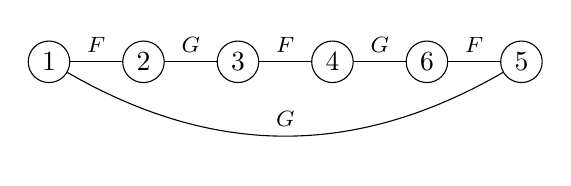
\begin{tikzpicture}[
                    scale=0.8,
                    vertex/.style={circle,
                    draw,
                    minimum size=1.5em,
                    inner sep=0pt,
                    align=center},
                    baseline=(1.base),
                    factor/.style={font=\footnotesize}
                ]
                    \node[vertex] (1) at (0,0) {$1$};
                    \node[vertex] (2) at (1.5,0) {$2$};
                    \node[vertex] (3) at (3,0) {$3$};
                    \node[vertex] (4) at (4.5,0) {$4$};
                    \node[vertex] (n3) at (6,0) {$6$};
                    \node[vertex] (n4) at (7.5,0) {$5$};
                    
                    \draw[factor] (1) -- node[above] {$F$} (2);
                    \draw[factor] (2) -- node[above] {$G$} (3);
                    \draw[factor] (3) -- node[above] {$F$} (4);
                    \draw[factor] (4) -- node[above] {$G$} (n3);
                    \draw[factor] (n3) -- node[above] {$F$} (n4);
                    \draw[factor] (n4) to[bend left=30] node[above] {$G$} (1);
                \end{tikzpicture}
            $$
            This proves the claim.
        \end{quote}

        \textbf{Claim 6.} \textit{Any\/ $1$-factorization is determined by two of its\/ $1$-factors. Reciprocally, any pair of edge-disjoint\/ $1$-factors can be extended to a unique\/ $1$-factorization.}

        \begin{quote}
            By Claim 5, after renaming the nodes, we may assume that $F\cup G$ consists of the sides of a hexagon. Therefore, the only possibilities left for the remaining $3$ $1$-factors are the three equilateral triangles whose sides skip one node.
        \end{quote}

        \textbf{Claim 7.} \textit{There are exactly\/ $6$ nonisomorphic\/ $1$-factorizations.}\footnote{Here ``isomorphisms'' are restricted to cyclic permutations of the six nodes, a.k.a. \textsl{rotations} as described below.}

        \begin{quote}
            As mentioned in Claim 4, after renaming the nodes we may assume that
            \begin{align*}
                F &= \{\{1,2\},\{3,4\},\{5,6\}\}\\
                G &= \{\{1,n_1\},\{2,n_2\},\{n_3,n_4\}\}
            \end{align*}
            Note that the permutation of nodes required to support this assumption implies that the only permutations that would produce equivalent $1$-factors are the rotations $\rho_t\colon i\mapsto\colon i\oplus_6t$.\footnote{Here $i\oplus_nj=i+j-1\pmod{n}+1$ is the cyclic sum.}
            
            By Claim 6, in order to count the number of $1$-factorizations it is enough to count the number of possible $1$-factors $G$, edge-disjoint from~$F$.
            
            Clearly $n_1\in\set{3,4,5,6}$. Moreover, taking into account that $\{n_3,n_4\}\ne\{5,6\}$ and $\{n_3,n_4\}\ne\{3,4\}$, we have
            $$
                \begin{tikzpicture}[
                    % General style for text in nodes
                    node_style/.style={font=\small}, 
                    % Styles for nodes at each level
                    n1_node/.style={node_style},
                    n2_node/.style={node_style}, % Added slight styling
                    g_node/.style={node_style},
                    % Style for the curved edges (branches)
                    branch_edge/.style={draw=black!70, -{Circle[length=1.5mm]}}
                    ]
                
                    % --- Define Y offsets for the main branches and sub-branches to control spacing ---
                    \def\yLevelOneSep{1.3cm}  % Vertical separation between n1=... blocks
                    \def\yLevelTwoSep{0.6cm}  % Vertical separation between n2=... sub-blocks within an n1 block
                    \def\xLevelSepOne{1.0cm} % Horizontal distance from (implicit) root to n1 nodes
                    \def\xLevelSepTwo{0.8cm} % Horizontal distance from n1 to n2 nodes
                    \def\xLevelSepThree{0.5cm}% Horizontal distance from n2 to G_i nodes
                    
                    % --- Invisible Root Node (for the main branches) ---
                    \coordinate (ImplicitRoot) at (-0.5, 0); % Positioned to the left, centered vertically
                    
                    % === n1=3 Branch ===
                    \node (n1_3) [n1_node] at (\xLevelSepOne, 1.5*\yLevelOneSep) {$n_1=3$};
                        \node (n2_3_5) [n2_node, right=\xLevelSepTwo of n1_3, yshift=0.5*\yLevelTwoSep] {$n_2=5$};
                            \node (G1) [g_node, right=\xLevelSepThree of n2_3_5] {$G_1 =\{\{1,3\},\{2,5\},\{4,6\}\}$};
                            \draw[dotted,-latex] (n2_3_5.east) to (G1.west);
                        \node (n2_3_6) [n2_node, right=\xLevelSepTwo of n1_3, yshift=-0.5*\yLevelTwoSep] {$n_2=6$};
                            \node (G2) [g_node, right=\xLevelSepThree of n2_3_6] {$G_2 =\{\{1,3\},\{2,6\},\{4,5\}\}$};
                            \draw[dotted,-latex] (n2_3_6.east) to (G2.west);
                        % Curved edges from n1_3 to its n2 children
                        \draw[branch_edge] (n1_3.east) to[out=25, in=180, looseness=2.0] (n2_3_5.west);
                        \draw[branch_edge] (n1_3.east) to[out=-25, in=-180, looseness=2.0] (n2_3_6.west);
                    
                    % === n1=4 Branch ===
                    \node (n1_4) [n1_node] at (\xLevelSepOne, 0.5*\yLevelOneSep) {$n_1=4$};
                        \node (n2_4_5) [n2_node, right=\xLevelSepTwo of n1_4, yshift=0.5*\yLevelTwoSep] {$n_2=5$};
                            \node (G3) [g_node, right=\xLevelSepThree of n2_4_5] {$G_3 =\{\{1,4\},\{2,5\},\{3,6\}\}$};
                            \draw[dotted,-latex] (n2_4_5.east) to (G3.west);
                        \node (n2_4_6) [n2_node, right=\xLevelSepTwo of n1_4, yshift=-0.5*\yLevelTwoSep] {$n_2=6$};
                            \node (G4) [g_node, right=\xLevelSepThree of n2_4_6] {$G_4 =\{\{1,4\},\{2,6\},\{3,5\}\}$};
                            \draw[dotted,-latex] (n2_4_6.east) to (G4.west);
                        \draw[branch_edge] (n1_4.east) to[out=25, in=180, looseness=2.0] (n2_4_5.west);
                        \draw[branch_edge] (n1_4.east) to[out=-25, in=-180, looseness=2.0] (n2_4_6.west);
                    
                    % === n1=5 Branch ===
                    \node (n1_5) [n1_node] at (\xLevelSepOne, -0.5*\yLevelOneSep) {$n_1=5$};
                        \node (n2_5_3) [n2_node, right=\xLevelSepTwo of n1_5, yshift=0.5*\yLevelTwoSep] {$n_2=3$};
                            \node (G5) [g_node, right=\xLevelSepThree of n2_5_3] {$G_5 =\{\{1,5\},\{2,3\},\{4,6\}\}$};
                            \draw[dotted,-latex] (n2_5_3.east) to (G5.west);
                        \node (n2_5_4) [n2_node, right=\xLevelSepTwo of n1_5, yshift=-0.5*\yLevelTwoSep] {$n_2=4$};
                            \node (G6) [g_node, anchor=base west] at ([xshift=\xLevelSepThree]n2_5_4.base east) {$G_6 =\{\{1,5\},\{2,4\},\{3,6\}\} \overset{\rho_1}\cong G_1$};       
                            \draw[dotted,-latex] ([yshift=2pt]n2_5_4.base east) to ([yshift=2pt]G6.base west);
                        \draw[branch_edge] (n1_5.east) to[out=25, in=180, looseness=2.0] (n2_5_3.west);
                        \draw[branch_edge] (n1_5.east) to[out=-25, in=-180, looseness=2.0] (n2_5_4.west);
                    
                    % === n1=6 Branch ===
                    \node (n1_6) [n1_node] at (\xLevelSepOne, -1.5*\yLevelOneSep) {$n_1=6$};
                        \node (n2_6_3) [n2_node, right=\xLevelSepTwo of n1_6, yshift=0.5*\yLevelTwoSep] {$n_2=3$};
                            \node (G7) [g_node, right=\xLevelSepThree of n2_6_3] {$G_7 =\{\{1,6\},\{2,3\},\{4,5\}\}$};
                            \draw[dotted,-latex] (n2_6_3.east) to (G7.west);
                        \node (n2_6_4) [n2_node, right=\xLevelSepTwo of n1_6, yshift=-0.5*\yLevelTwoSep] {$n_2=4$};
                            \node (G8) [g_node, anchor=base west] at ([xshift=\xLevelSepThree]n2_6_4.base east) {$G_8 =\{\{1,6\},\{2,4\},\{3,5\}\} \overset{\rho_2}\cong G_2$};
                            \draw[dotted,-latex] ([yshift=2pt]n2_6_4.base east) to ([yshift=2pt]G8.base west);
                        \draw[branch_edge] (n1_6.east) to[out=25, in=180, looseness=2.0] (n2_6_3.west);
                        \draw[branch_edge] (n1_6.east) to[out=-25, in=-180, looseness=2.0] (n2_6_4.west);
                \end{tikzpicture}
            $$
            where $\rho_1(i)=i\oplus_61$ and $\rho_2(i)=i\oplus_62$ are the rotations. As can be easily verified, no other cyclic isomorphism $\rho_t$ identifies the remaining $6$ factorizations. The claim follows.
        \end{quote}

        Let $\mathcal Q$ be the set of points in $\Pi$ external to $\mathcal O$. To each $R\in\mathcal Q$, we can associate the following map
        \begin{align*}
            f_R\colon\mathcal O&\to\mathcal O\\
            A_i&\mapsto RA_i\cap(\mathcal O\setminus\{A_i\})
        \end{align*}
        that assigns the second point of intersection between $RA_i$ and $\mathcal O$. By Claim~3, $f_R$ ---think of it as a set--- can be identified with a (unique) $1$-factor of $K_6$, namely $\set{\{A_i,f_R(A_i)\}\mid 1\le i\le 6}$.\footnote{Incidentally, $f_R\circ f_R=\id_{\mathcal O}$.}

        Let $\Phi$ be the set of $1$-factors of $K_6$. The map
        \begin{align}\label{function:f}
            f\colon\mathcal Q&\to\Phi\\
            R&\mapsto f_R
        \end{align}
        is injective because any pair of secants in $f_R$ intersect at $R$. It is also surjective because, according to \eqref{eq:15-patitions}, $|\Phi|=15$ and $|\mathcal Q|=21-|\mathcal O|=15$.

        Let $\mathcal M$ be the set of lines missing $\mathcal O$. If a line meets $\mathcal O$, it does at exactly $2$ points. Therefore, there are $\binom62=15$ of them. In consequence, there are $21-15=6$ lines missing $\mathcal O$, i.e., $|\mathcal M|=6$.
        
        Let $\block r\in\mathcal M$. If $R$ and $S$ are two points in $\block r$, then $f_R\cap f_S=\emptyset$. Indeed,
        \begin{align*}
            \{A_i,f_R(A_i)\}=\{A_j,f_S(A_j)\}
                &\implies A_i=A_j \text{ and }f_R(A_i)=f_S(A_i)\\
                &\implies R,S\in A_if_R(A_i)=A_jf_S(A_j)\\
                &\implies \block r=RS=A_if_R(A_i)\\
                &\implies A_i\in\block r\ \noend
        \end{align*}
        In consequence, if $\Theta$ is the set of $1$-factorizations of $K_6$, the function $f$ defined in \eqref{function:f} induces a map
        \begin{align*}
            f_*\colon\mathcal M&\to\Theta\\
            \block r&\mapsto f(\block r),
        \end{align*}
        where $\block r$ is identified with the set of its $5$ points, and $f(\block r)$ is the set-image of such points.
        
        The function $f_*$ is injective because the $3$ secants in each $1$-factor intersect at the same point. It is also surjective since, by Claim~7, $|\Theta|=6$ and, as we have seen, $|\mathcal M|=6$.

        For the points of $\mathcal O$ we simply define
        \begin{align*}
            g\colon\mathcal O&\to\op N(K_6)\\
            A_i&\mapsto i,
        \end{align*}
        where $\op N(K_6)$ stands for the nodes of $K_6$ and $i$ for the $i$th node, which is clearly bijective.

        Let $\mathcal H$ be the set of lines meeting $\mathcal O$. If $\op E(K_6)$ denotes the set of edges of $K_6$, we can define
        \begin{align*}
            g_*\colon\mathcal H&\to\op E(K_6)\\
            A_iA_j &\mapsto \{i,j\},
        \end{align*}
        Combining all these maps we have a bijection
        \begin{align*}
            f\cup g\times f_*\cup g_*\colon
                \underbrace{\mathcal Q\cup\mathcal O}_{\pts}
                \times\underbrace{\mathcal M\cup\mathcal H}_{\blocks}
                &\to \Phi\cup\op N(K_6)\times\Theta\cup\op E(K_6),
        \end{align*}
        where $\pts$ denotes the points of $\Pi$ and $\blocks$ its lines.

        \textbf{Conclusion.} Given the bijection above between the points and lines of $\Pi$ and an independent structure built on intrinsic features of $K_6$, any other projective plane would be equipped with a similar bijection. However, any two models for $K_6$ are isomorphic through a permutation of nodes, the inverse of the second bijection composed with the first, results in an isomorphism between both projective planes.

        \item[Order $5$.] ??? \qedhere
    \end{description}
\end{solution}

\begin{exr}
    Prove that the order of\/ $\PG(2,q)$ is\/ $q$.
\end{exr}

\begin{solution}
    See Remark~\ref{rem:order-of-galois-plane}.
\end{solution}


\begin{exr} {\upshape[Kárteszi]}
    Determine the size of the incidence tables obtained in the rounds of Hall’s free extension process.
\end{exr}

\textbf{Note.} This is also Exercise 8 -- page 79 -- of \textit{Introduction to Finite Geometries} by F. Kárteszi.

\begin{solution}
    We start by being more precise about the inductive construction given in Example~\ref{xmpl:hall-plane}.
    
    Let $\Pi_n=(\pts_n,\blocks_n,\incidence_n)$ be the incidence geometry induced by the incidence table $T_n$, as defined in Example~\ref{xmpl:hall-plane}. Since $T_n$ is a block inside $T_{n+1}$, $\Pi_n$ is an incidence subgeometry of $\Pi_{n+1}$. The first table $T1$ corresponds to an incidence geometry $\Pi_1$ that satisfies P1 and P3' (or \PP2 and P3'' if transposed). As we observed in the example, P3' (respectively, P3'') is satisfied by all subsequent geometries.

    \textbf{Claim 1.} \textit{Every $\Pi_n$ is a partial projective plane, i.e., it satisfies axioms\/~{\upshape P1'} and\/~{\upshape P2'}.}

    By induction on $n$. The case $n=1$ is actually a requirement to start the process. For $n>1$, suppose that $\Pi_{n-1}$ is a partial projective plane. There are three possibilities
    \begin{enumerate}[a),font=\upshape]
        \item \textit{$\Pi_n$ is a projective plane}. In this case, the process would make $\Pi_{n+1}=\Pi_n$, which is a projective plane, in particular a partial one.
        \item \textit{$\Pi_n$ does not satisfy} \PP2. In this case, $T_{n+1}$ adds to $T_n$ new columns that correspond to the intersections of existing lines that had no point in common in $\Pi_n$. This addition preserves P1' and P2' because no lines are added.
        \item \textit{$\Pi_n$ does not satisfy} \PP1. Then its dual does not satisfy \PP2 and the conclusion follows from the previous possibility.
    \end{enumerate}

    \bigskip
    
    \textbf{Claim 2.} \textit{No\/ $\Pi_n$ is a projective plane.}
    
    We proceed by induction on\/ $n$.
    
    \begin{enumerate}[a),font=\upshape]
    \item \textit{Base case.} For $n=1$, the claim is clear: $\Pi_1$ trivially fails to satisfy at least one of the axioms~\PP1 and \PP2.
    \item \textit{Inductive step.} Suppose that $\Pi_n$ is not a projective plane. We consider the two possible reasons:
      \begin{enumerate}[i),font=\upshape]
          \item If\/ $\Pi_n$ fails axiom~\PP2, then the table $T_{n+1}$ adds new columns to $T_n$, each of which represents a point in $\pts_{n+1}\setminus\pts_n$. By construction, these new points are incident with exactly two lines already present in $\blocks_n$ that had no intersection in $\Pi_n$. As a result, these new points are incident with only two lines, so certainly not with at least three, violating axiom~\PP1. Therefore, $\Pi_{n+1}$ is not a projective plane.
        
          \item If\/ $\Pi_n$ fails axiom~\PP1, the conclusion follows from part~(i), but applied to the sequence of transposed incidence tables, which defines the dual geometries.
      \end{enumerate}
    \end{enumerate}

    \bigskip

    \textbf{Claim 3.} \textit{The union\/ $\Pi=\bigcup\set{\Pi_n\mid n\ge1}$ is a projective plane.}

    As we mentioned above, $\Pi$ satisfies P3' or P3''. In consequence, we must show that it also satisfies \PP1 and \PP2. To see $P_1$, take two points $A$ and $B$ in $\Pi$. Let 
    $$
        n=\max\set{k\mid A,B\in\pts_k}.
    $$
    By construction, $\Pi_n$ satisfies P1' and P2', as defined in \ref{xmpl:hall-plane}. Therefore, if~$A$ and $B$ violate P1, then $T_{n+1}$ will add one, and only one, row to $T_n$ representing a line in~$\blocks_{n+1}$, incident with $A$ and with $B$. Thus, $A$ and $B$ define a unique line in $\Pi_{n+1}$ and, \textit{a fortiori}, in $\Pi$ by virtue of~P1'. Thus, $\Pi$ satisfies \PP1. The dual construction shows that $\Pi$ also satisfies~\PP2.

    \bigskip

    \textbf{Notation.} Let's introduce the following quantities associated to $\Pi_n$
    \begin{enumerate}[-]
        \item $d_n = \#\{\text{disjoint pairs of lines}\}$,
        \item $e_n = \#\{\text{non-collinear pairs of points}\}$,
        \item $q_n = \#\max\{\text{points per line}\}$,
    \end{enumerate}
    to which we add $v_n=|\pts_n|$ and $b_n=|\blocks_n|$.
    
    The first values are:
    \begin{center}
        \begin{tabular}{l|ccccc}
             &$1$&$2$&$3$&$4$&$\cdots$\\
             \hline
             $d_n\rule{0pt}{10pt}$&$3$&$0$&$6$&$0$&$\cdots$\\
             $e_n$&$0$&$3$&$0$&$24$&$0$\\
             $b_n$&$6$&$6$&$9$&$9$&$33$\\
             $v_n$&$4$&$7$&$7$&$13$&$13$
        \end{tabular}
    \end{center}
    Moreover
    $$
        v_{n+1}=v_n+d_n,\quad b_{n+1}=b_n+e_n.
    $$
    Given a pair of disjoint lines, say $\block a$ and $\block b$, the algorithm adds a new point~$P$ to both of them, attaching a new column to the table with exactly two $1$s. If a third line $\block c$ is disjoint from $\block a$ (or $\block b$ or both), the algorithm adds a point $Q$ to both of them as well. The key observation is that $P\ne Q$. Otherwise, the addition of $P$ would have created an ``accidental'' incidence, which goes against the \textit{free} nature of the process. Hence, the equation $v_{n+1}=v_n+d_n$. The dual consideration translates as $b_{n+1}=b_n+e_n$.

    ???

\end{solution}

\begin{exr}
    Use the process indicated in\/ {\upshape Theorem~\ref{thm:mols-equivalence}} to construct explicitly a complete set of\/ $\mols$, starting from the plane\/~$\PG(2,q)$.
\end{exr}

\begin{solution}
    Let $\Fq=\set{\zeta_0,\dots,\zeta_{q-1}}$, where $\zeta_0=0$ and $\zeta_1=1$. With the notation of the theorem, and recalling that $n=q$, let $\ell$ be defined by the equation $z=0$, $X=[1:0:0]$, $Y=[0:1:0]$ and $M=[1:1:0]$. Then, for $1\le i,j\le q$, we have
    $$
        \block h_i\equiv y-\zeta_{i-1} z=0,\quad\block v_j\equiv x-\zeta_{j-1} z=0.
    $$
    Thus,
    $$
        \lambda(i,j)=\block h_i\wedge\block v_j
            =[\zeta_{j-1},\zeta_{i-1},1].
    $$
    Moreover,
    $$
        \tr(\ell)\setminus\set{X,Y}
            = \set{[1:\zeta_1:0],\dots,[1:\zeta_{q-1}:0]}
            \quad\text{or}\quad M_m=[1:\zeta_m:0]
    $$
    and
    $$
        \pl(M_m)\setminus\set\ell
            =\set{\zeta_mx-y+\zeta_{k-1}z=0\mid 1\le k\le q},
    $$
    i.e.,
    $$
        \block m_k\equiv\zeta_mx-y+\zeta_{k-1}z=0.
    $$
    It follows that
    \begin{align}\label{eq:iota_m}
        [\zeta_{j-1}:\zeta_{i-1}:1]\incidence\block m_k
            &\iff\zeta_m\zeta_{j-1}-\zeta_{i-1}+\zeta_{k-1}=0
                \nonumber\\
            &\iff \zeta_{k-1}=\zeta_{i-1}-\zeta_m\zeta_{j-1}.
    \end{align}
    Hence,
    \begin{align*}
        L_m(i,j) &= \sigma_m\circ\iota_m\circ\lambda(i,j)\\
            &= \sigma_m\circ\iota_m([\zeta_{j-1},\zeta_{i-1},1])\\
            &= \sigma_m(\block m_k)\\
            &= k-1,
    \end{align*}
    where $\zeta_{k-1}$ is defined in \eqref{eq:iota_m}.
    
\end{solution}

%\newpage
\begin{test}
    Let $\Fq[2^2]=\set{0,1,\iq,\iq^2}$ be the field of $4$ elements [cf.~Exercise~\ref{exr:order-4=PG(2,4)}]. For $m=1$, we have to compute the values of $\zeta_{k-1}=\zeta_{j-1}+\zeta_{i-1}$
    $$
        \begin{bmatrix}
            0   &1  &\iq  &\iq^2\\
            1   &0  &\iq^2&\iq\\
            \iq   &\iq^2&0  &1\\
            \iq^2 &\iq  &1  &0
        \end{bmatrix}
        \quad\longrightarrow\quad
        L_1 = \begin{bmatrix}
            0   &1  &2  &3\\
            1   &0  &3  &2\\
            2   &3  &0  &1\\
            3   &2  &1  &0
        \end{bmatrix}
    $$
    For $m=2$ the equation is $\zeta_{k-1}=\zeta_{i-1}+\iq\zeta_{j-1}$
    $$
        \begin{bmatrix}
            0   &\iq    &\iq^2  &1\\
            1   &\iq^2  &\iq    &0\\
            \iq &0      &1      &\iq^2\\
            \iq^2&1     &0      &\iq
        \end{bmatrix}
        \quad\longrightarrow\quad
        L_2 = \begin{bmatrix}
            0   &2  &3  &1\\
            1   &3  &2  &0\\
            2   &0  &1  &3\\
            3   &1  &0  &2
        \end{bmatrix}
    $$
    For $m=3$ the equation is $\zeta_{k-1}=\zeta_{i-1}+\iq^2\zeta_{j-1}$
    $$
        \begin{bmatrix}
            0   &\iq^2  &1      &\iq\\
            1   &\iq    &0      &\iq^2\\
            \iq &1      &\iq^2  &0\\
            \iq^2&0     &\iq    &1
        \end{bmatrix}
        \quad\longrightarrow\quad
        L_3 = \begin{bmatrix}
            0   &3  &1  &2\\
            1   &2  &0  &3\\
            2   &1  &3  &0\\
            3   &0  &2  &1
        \end{bmatrix}
    $$
    Orthogonality between $L_1$ and $L_2$:
    $$
        (L_1,L_2) = \begin{bmatrix}
            (0,0)   &(1,2)   &(2,3)   &(3,1)\\
            (1,1)    &(0,3)   &(3,2)   &(2,0)\\
            (2,2)    &(3,0)   &(0,1)   &(1,3)\\
            (3,3)    &(2,1)   &(1,0)   &(0,2)
        \end{bmatrix}
    $$
    Orthogonality between $L_1$ and $L_3$:
    $$
        (L_1,L_2) = \begin{bmatrix}
            (0,0)   &(1,3)   &(2,1)   &(3,2)\\
            (1,1)    &(0,2)   &(3,0)   &(2,3)\\
            (2,2)    &(3,1)   &(0,3)   &(1,0)\\
            (3,3)    &(2,0)   &(1,2)   &(0,1)
        \end{bmatrix}
    $$
    Orthogonality between $L_2$ and $L_3$:
    $$
        (L_1,L_2) = \begin{bmatrix}
            (0,0)   &(2,3)   &(3,1)   &(1,2)\\
            (1,1)    &(3,2)   &(2,0)   &(0,3)\\
            (2,2)    &(0,1)   &(1,3)   &(3,0)\\
            (3,3)    &(1,0)   &(0,2)   &(2,1)
        \end{bmatrix}
    $$
\end{test}

\textbf{Formalization.} For a formalization of the general case of $\mols$ of order $q=p^n$ see \citep{BurroniFiniteGeometryRepo}.

\begin{exr}
    A\/ $2$-$(v, k, \lambda)$-design is called \textsl{square} (or \textsl{symmetric}) if it has as many points as blocks (formally:\/ $b = v$). Show that a design is square if, and only if, $r = k$. Show that in a square design two blocks intersect in exactly\/ $\lambda$ points. {\upshape Hint: Show that\/ $AA^T = A^T\!A$.}
\end{exr}

\begin{solution} We provide two solutions from two different sources

    \citep{Chowla_Ryser_1950} Assume that $v=b$. By Exercise~\ref{exr:design-basic-combinatory}, we also know that $k=r$. Define the matrix
    $$
        \Omega = \begin{pmatrix}
            -k  &\sqrt{-\lambda}    &\cdots &\sqrt{-\lambda}\\
            \sqrt{-\lambda}\\
            \vdots  &   &\textit{\Large A}\\
            \vdots\\
            \sqrt{-\lambda}
        \end{pmatrix}
    $$
    Let $\Omega_0$ be the $(v+1)\times(v+1)$ matrix whose first row and column equal the same row and column of $\Omega$ and all entries occupied by $A$ are zero. Then enlarge $A$ to $A_0$ by adding one row and one column with zeros as entries. We can decompose $\Omega$ into the sum
    
    \footnotesize
    \begin{align*}
        \Omega &= \Omega_0 + A_0
            = \begin{pmatrix}
                    -k&\sqrt{-\lambda}&\cdots&\sqrt{-\lambda}\\
                    \sqrt{-\lambda}\\
                    \vdots&&\textit{\Large 0}\\
                    \vdots\\
                    \sqrt{-\lambda}
                \end{pmatrix}
                +
                \begin{pmatrix}
                    0&0&\cdots&0\\
                    0\\
                    \vdots  &   &\textit{\Large A}\\
                    \vdots\\
                    0
                \end{pmatrix}
    \end{align*}
    \normalsize
    Before computing $\Omega^T\Omega$, let's observe the following
    \begin{align*}
        k^2-v\lambda &= k^2-\frac{k(k-1)}{v-1}v
            &&\text{; Exer.~\ref{exr:design-basic-combinatory}}\\
            &= \frac{k^2(\cancel v-1)-k(\cancel k-1)v}{v-1}\\
            &= \frac{kv-k^2}{v-1}
        \intertext{and}
        k-\lambda &= k - \frac{k(k-1)}{v-1}\\
            &= \frac{k(v-1)-k(k-1)}{v-1}\\
            &= \frac{kv-k^2}{v-1}.
    \end{align*}
    Hence,
    \begin{equation}\label{eq:OmegaTOmega-11}
        k^2-v\lambda=k-\lambda.
    \end{equation}
    We can now compute $\Omega^T\Omega$ as follows
    \begin{align*}
        \Omega^T\Omega &= \Omega_0\Omega_0 + \Omega_0A_0
                + (\Omega_0A_0)^T + A_0^TA_0\\
    \end{align*}
    where
    \footnotesize
    \begin{align*}
        \Omega_0\Omega_0 &= \begin{pmatrix}
            k^2-v\lambda
                &-k\sqrt{-\lambda}&\cdots&-k\sqrt{-\lambda}\\
            -k\sqrt{-\lambda}\\
            \vdots&&\text{\large $-\lambda U$}\\
            -k\sqrt{-\lambda}
        \end{pmatrix},\\
        \Omega_0A_0 &= \begin{pmatrix}
            0&k\sqrt{-\lambda}&\cdots&k\sqrt{-\lambda}\\
            0\\
            \vdots&&\text{\large$0$}\\
            0
        \end{pmatrix}\\
        A^T_0A_0 &= \begin{pmatrix}
            0&\cdots&0\\
            \vdots&\text{\large$(k-\lambda)I+\lambda U$}\\
            0
        \end{pmatrix}
    \end{align*}
    \normalsize
    In combination with \eqref{eq:OmegaTOmega-11}, we obtain
    \begin{equation}\label{eq:k-lambda-is-a-square}
        \Omega^T\Omega=(k-\lambda)I,
    \end{equation}
    which implies $\Omega^T\Omega^T=\Omega\Omega^T$. Thus,
    $$
        \Omega_0A_0+(\Omega_0A_0)^T + A_0^TA_0
        = \Omega_0A_0^T+(\Omega_0A_0^T)^T+A_0A_0^T.
    $$
    Since every vector $(0,x_1,\dots,x_v)$ is in the kernel of $\Omega_0$, we see that $\Omega_0A_0$ and $\Omega_0A_0^T$ are both zero. Therefore, $A_0^TA_0=A_0A_0^T$ and so $A^T\!A=AA^T$.

    By Exercise~\ref{exr:design-incidence-matrix}, we deduce that all block intersections $\block a_i\cap\block a_j$, $i\ne j$, have~$\lambda$ points.
    
\separator

    \citep{Stinson2004}
    Let $A$ be the incidence matrix of the design, where rows represent blocks and columns points. According to Exercise~\ref{exr:design-incidence-matrix}
    \begin{equation}\label{eq:AA^T2}
        (AA^T)_{ij} = \sum_{h=1}^va_{ih}a_{jh}
            = \begin{cases}
                k   &\text{if }i=j,\\
                |\block a_i\cap\block a_j|
                    &\text{if }i\ne j.
            \end{cases}
    \end{equation}
    For $1\le i\le b$, let $\vect a_i$ denote the $i$th row of $A$, considered as an element in $\Q^v$. As shown in Exercise~\ref{exr:design-incidence-matrix},
    the linear map $\vect x\mapsto A\vect x$ is a monomorphism from $\Q^v$ to $\Q^b$.

    \textbf{Lemma.} \textit{With the previous notation, let\/ $\set{\block a_1,\dots,\block a_b}$ and\/ $\set{A_1,\dots,A_v}$ be, respectively, the blocks and points of the design. Then}
    \begin{equation}\label{eq:sum-of-inicidence-rows}
        \sum_{i=1}^b\vect a_i = (r,\dots,r)
        \quad\text{and}\quad
        \sum_{\{i\,\mid\,A_j\in\block a_i\}}\!\!\!\!\!\vect a_i=(r-\lambda)\vect e_j+(\lambda,\dots,\lambda),
    \end{equation}
    \textit{where\/ $\vect e_j$ is the\/ $j$th canonical vector of\/ $\Q^v$, $1\le j\le v$.}

    \small
    \textsc{Proof.} The first equality is clear because at each coordinate the sum counts the number of blocks incident with the point represented by said coordinate. By definition, this is~$r$.

    For the second equality, first consider the $j$th coordinate, i.e., the one corresponding to $A_j$. Since the sum runs over all blocks incident with $A_j$, coordinate $j$ counts the number of such blocks, that is $r$. For any other coordinate $h\ne j$, the sum counts all blocks incident with $A_j$ and $A_h$. This, by definition, is $\lambda$.\hfill\rule{0.6em}{0.6em}
    
    \normalsize    
    \bigskip
    As a consequence of the lemma, for $1\le h\le b$, we have
    \begin{align*}
        \sum_{\{j\,\mid\,A_j\in\block a_h\}}
            \sum_{\{i\,\mid\,A_j\in\block a_i\}}\!\!\!\!\!\vect a_i
            &\;= \!\!\!\!\!\sum_{\{j\,\mid\,A_j\in\block a_h\}}
                (r-\lambda)\vect e_j+(\lambda,\dots,\lambda)\\
            &\;= (r-\lambda)\vect a_h+k(\lambda,\dots,\lambda)\\
            &\;= (r-\lambda)\vect a_h + \frac{k\lambda}r
                \sum_{i=1}^b\vect a_i.
    \end{align*}
    On the other hand,
    \begin{align*}
    \sum_{\{i\,\mid\,A_j\in\block a_i\}}
            \sum_{\{j\,\mid\,A_j\in\block a_h\}}\!\!\!\!\!\vect a_i
            &=\; \sum_{i=1}^b
                \sum_{\{j\,\mid\,A_j\in\block a_i\cap\block a_h\}}
                \!\!\!\!\!\vect a_i\\
            &=\; \sum_{i=1}^b|\block a_i\cap\block a_h|\vect a_i.
    \end{align*}
    Hence,
    $$
        (r-\lambda)\vect a_h + \frac{k\lambda}r
                \sum_{i=1}^b\vect a_i
            = \sum_{i=1}^b|\block a_i\cap\block a_h|\vect a_i
    $$
    or
    $$
        \Big(r-\lambda +\frac{k\lambda}r-k\Big)\vect a_h
            = \sum_{i=1,i\ne h}^b
                \Big(|\block a_i\cap\block a_h|-\frac{k\lambda}r\Big)
                    \vect a_i
    $$
    and we get the following linear relations
    $$
        (r-\lambda)(r-k)\vect a_h
            = \sum_{i=1,i\ne h}^b
                (r|\block a_i\cap\block a_h|-k\lambda)
                    \vect a_i.
    $$
    In the case $v=b$, by Exercise~\ref{exr:design-basic-combinatory}, we know that $k=r$ and the rows of $A$ are linearly independent. It follows that $|\block a_i\cap\block a_h|=\lambda$ for all $i\ne h$.

    Conversely, if $|\block a_i\cap\block a_h|=\lambda$ whenever $i\ne h$, the relation above translates into
    $$
        (r-\lambda)(r-k)\vect a_h
            = \lambda(r-k)\sum_{i=1,i\ne h}^b\vect a_i.
    $$
    Hence, $r=k$ and so $v=b$ or
    $$
        r\vect a_h = \lambda(r,\dots,r).
    $$
    By~\eqref{eq:sum-of-inicidence-rows}, this equality implies that\/ $\vect a_h = (1,\dots,1)$ for all\/ $h$, which is only possible if every point lies in every block—that is, the design is a\/ $(v,v,v)$-design, hence square.

    Finally note that equations \eqref{eq:A^TA} and \eqref{eq:AA^T} show that the design is square if, and only if, $A^T\!A=AA^T$.
    
\end{solution}

\begin{exr}
    Extend the Bruck--Ryser\/ {\upshape Theorem~\ref{thm:bruck-ryser}} to square designs with odd\/ $v$ by proving that the Diophantine equation
    \[
        x^2 = (k - \lambda)y^2 + (-1)^{(v-1)/2}\lambda z^2
    \]
    admits a nontrivial integer solution different from\/ $(0,0,0)$.
    
    \textrm{\upshape Hint: Try to copy the proof of the Bruck--Ryser theorem; for\/ $v \equiv 3 \pmod{4}$ introduce the new indeterminate\/ $x_{v+1}$ while for\/ $v \equiv 1 \pmod{4}$ separate the last variable and use Lagrange's identity for four consecutive terms as in the original proof.}
\end{exr}

\begin{solution}
    In the square case, where $v=b$ and $r=k$, we have
    \begin{align*}
        (\det A)^2 &= \det(A^TA)\\
            &= (k+(v-1)\lambda)(r-\lambda)^{v-1}
                &&\text{; Exer.~\ref{exr:design-incidence-matrix}}\\
            &= (k+k(k-1))(k-\lambda)^{v-1}
                &&\text{; Exer.~\ref{exr:design-basic-combinatory}}\\
            &= k^2(k-\lambda)^{v-1}.
    \end{align*}
    If $v$ is even, the equality above shows that $k-\lambda$ is a perfect square.\footnote{This is also a consequence of \eqref{eq:k-lambda-is-a-square}.}

    If $v$ is odd, there are two cases: 1)~$v\equiv1\bmod 4$ and 2)~$v\equiv3\bmod 4$.

    \begin{description}
        \item[Case 1.] Let $A$ denote the incidence matrix of the design. Consider the equation $\mathtt y=A\mathtt x$, where $\mathtt x=(x_1,\dots,x_v)$ and $\mathtt y=(y_1,\dots,y_v)$. Then
        \begin{align*}
            y_1^2+\cdots+y_v^2 &= \mathtt y^T\mathtt y\\
                &= \mathtt x^TA^T\!A\mathtt x\\
                &= \mathtt x^T((k-\lambda)I
                    +\lambda U)\mathtt x\\
                &= (k-\lambda)(x_1^2+\cdots+x_v^2) 
                    +\lambda(x_1+\cdots+x_v)^2\\
                &= (k-\lambda)(x_1^2+\cdots+x_v^2) + \lambda w^2,
        \end{align*}
        where $w=(1,\dots,1)^T\mathtt x$. Since $4\mid v-1$, we can group the elements $x_1,\dots, x_{v-1}$ into $(v-1)/4$ parts of $4$ terms with consecutive indexes each: $x_{4i+1},x_{4i+2},x_{4i+3},x_{4i+4}$ for $0\le i\le v-1$. 
        
        Since $k=r=\lambda(v-1)/(k-1)\ge\lambda$, because $v\ge k$, we can replace $k-\lambda$ with a sum of $4$ squares and, according to Corollary~\ref{cor:nonsingular-4-square-matrix}, write
        $$
            z_{4i+1}^2+z_{4i+2}^2+z_{4i+3}^2+z_{4i+4}^2
                = (k-\lambda)(x_{4i+1}^2+x_{4i+2}^2+
                    x_{4i+3}^2+x_{4i+4}^2),
        $$
        where
        \begin{align*}
            (z_{4i+1},z_{4i+2},z_{4i+3},z_{4i+4})
                &= (k-\lambda)(x_{4i+1},x_{4i+2},x_{4i+3},x_{4i+4})\\
                &= B_i(x_{4i+1},x_{4i+2},x_{4i+3},x_{4i+4})
        \end{align*}
        for some nonsingular integer matrix $B_i$. Add $z_v=x_v$. If $B$ is the resulting $v\times v$ diagonal block matrix $\diag(B_1,\dots,B_{(v-1)/4)},1)$, then $B$ is nonsingular and
        $$
            \mathtt z=B\mathtt x.
        $$
        Thus, $\mathtt y = AB^{-1}\mathtt z$ and\/ $w = (1,\dots,1)^T B^{-1}\mathtt z$ express the linear dependence of\/ $\mathtt y$ and\/ $w$ on\/ $\mathtt z$, subject to the equation
        \[
            y_1^2 + \cdots + y_v^2
                = z_1^2 + \cdots + z_{v-1}^2 + (k - \lambda) z_v^2 + \lambda w^2.
        \]

        \item[Case 2.] Here $4\mid v+1$. Add the variables\/ $x_{v+1}$ and\/ $y_{v+1}=x_{v+1}$. In matrix form, this yields the equation\/ $\mathtt y=A'\mathtt x$, where\/ $A'=\diag(A,1)$. Hence, from $A^TA=(k-\lambda)I+\lambda U$, we get
        \[
            y_1^2+\cdots+y_v^2+(k-\lambda)y_{v+1}^2
                = (k-\lambda)(x_1^2+\cdots+x_{v+1}^2) + \lambda w^2,
        \]
        where $w=x_1+\cdots+x_{v+1}$. As in the first case, we can introduce $\mathtt z=B\mathtt x$, where $B$ is a nonsingular integer $(v+1)\times(v+1)$ matrix. The equation above translates into
        \[
            y_1^2+\cdots+y_v+(k-\lambda)y_{v+1}^2
                = z_1^2+\cdots+z_{v+1}^2 + \lambda w^2,
        \]
        where $y_1,\dots,y_{v+1}$ and $w$ are linear combinations of $x_1,\dots,x_{v+1}$ with coefficients in $\Q$.
        
    \end{description}

    \textbf{Lemma.} [cf.~Lemma~\ref{lem:quadratic-criterion-for-sum-of-squares}] \textit{Let\/ $a$ and $b$ be two integers, and $\zeta_1,\dots,\zeta_n$ linearly independent linear forms with coefficients in\/ $\Q$. Suppose\/ $\vartheta_1,\dots,\vartheta_n,\omega$ are\/ $\Q$-linear combinations of\/ $\zeta_1,\dots,\zeta_n$ satisfying}
    \begin{equation}\label{eq:minimum-n}
        \vartheta_1^2+\cdots+\vartheta_{n-1}^2
            + a\vartheta_n^2
            = \zeta_1^2+\cdots+\zeta_n^2 + b\omega^2,
    \end{equation}
    \textit{for some integer\/ $n$. Then\/ the equation\/ $ay^2=x^2+bz^2$ has a nontrivial solution in\/ $\Z$.}

    \small
    \needspace{3\baselineskip}
    \textsc{Proof.} Fix\/ $a$ and\/ $b$, and suppose that\/ $n$ is minimal with the property stated, for any possible sequence of linear forms. If\/ $n=1$, the conclusion is immediate because:
    \begin{enumerate}[-]
        \item the desired equation can be solved over $\Q$ by assigning any nonzero integer value to\/ $\zeta_1$ and then computing\/ $\omega$ and\/ $\vartheta_1$ accordingly, and  
        \item since the equation is homogeneous of degree\/ $2$, any rational solution can be scaled to yield an integer one.
    \end{enumerate}


    If $n>1$, write
    $$
        \vartheta_1 = c_1\zeta_1+\cdots+c_n\zeta_n.
    $$
    After replacing $\vartheta_1$ with $-\vartheta_1$, if necessary, we may assume that $c_1\ne1$. Introduce the linear form
    $$
        \theta=\frac1{1-c_1}\vartheta_1(0,\zeta_2,\dots,\zeta_n)
    $$
    and define
    \begin{align*}
        \bar\omega &= \omega(\theta,\zeta_2,\dots,\zeta_n),\\
        \bar\vartheta_i &= \vartheta_i(\theta,\zeta_2,\dots,\zeta_n)
            &&;\ 2\le i\le n.
    \end{align*}
    Since $\theta-c_1\theta=\vartheta_1-c_1\zeta_1$, we have
    \begin{align*}
        \bar\vartheta_1
            &= c_1\theta+c_2\zeta_2+\cdots+c_n\zeta_n\\
            &= \theta - \vartheta_1 + c_1\zeta_1
                + \vartheta_1 - c_1\zeta_1\\
            &= \theta.
    \end{align*}
    Therefore, evaluating \eqref{eq:minimum-n} at $(\theta,\zeta_2,\dots,\zeta_n)$, we get
    $$
        \cancel{\bar\vartheta_1^2}+\bar\vartheta_2^2\cdots+\bar\vartheta_{n-1}^2+a\bar\vartheta_n^2
            = \cancel{\theta^2}+\zeta_2^2+\cdots+\zeta_n^2
                +b\bar\omega^2.
    $$
    Thus, $\bar\vartheta_2,\dots,\bar\vartheta_{n-1}$ are rational linear forms in $\zeta_2,\dots,\zeta_n$ that contradict the minimality of~$n$.\hfill\rule{0.6em}{0.6em}
    
    \normalsize
    Note that the lemma can be applied directly to conclude the proof of Case~2. For Case~1 it is enough to observe that the roles of $\mathtt y$ and $\mathtt z$ can be interchanged because both matrices, $A$ and $B$, are nonsingular, which allows all involved linear forms to be expressed as linear combinations of $y_1,\dots,y_v$. The solution is now complete.

    \small
    \textbf{Corollary.} \textit{If\/ $v$ is odd, and there exists an odd prime\/ $p$ dividing the squarefree part of\/ $k - \lambda$ such that\/ $(-1)^{(v-1)/2}\lambda$ is not a square in\/ $\Z/p\Z$, then no $2$-$(v,k,\lambda)$ square design exists.}

    \textsc{Proof.} By the lemma above, if such a design existed, the Diophantine equation $(k-\lambda)y^2=x^2+(-1)^{(v-1)/2}\lambda z^2$ would have a nontrivial integer solution. Without loss of generality we may assume that $x$, $y$, and $z$ have no common factors. Write $k-\lambda=pq$, with $p\perp q$. Then $p\nmid z$ and $(-1)^{(v-1)/2}\lambda=(z^{-1}x)^2$ in $\Z/p\Z$, in contradiction with the hypothesis.%\hfill\rule{0.5em}{0.5em}

    \textbf{Example.} \textit{There is no projective plane of order $6$.}

    Otherwise, we would have $v=43$, $k=7$ and $\lambda=1$, with $(v-1)/2=21$ odd. Since $k-\lambda=6$, we can take $p=3$ and verify that $-\lambda=2\ne1$ in $\Z/3\Z$ is not a square.
    
    \normalsize
\end{solution}

\begin{exr}
     Show that the Moulton plane\/ {\upshape[Example~\ref{xmpl:affine-moulton}]} is not Desarguesian.
\end{exr}

\begin{solution}
    Consider the following three Moulton lines:
    \begin{align*}
        y &= -x+1, &x &= 0, &y = \begin{cases}
            x+2 &\text{if }x<-2,\\
            \frac12 x+1 &\text{if }x\ge-2.
        \end{cases} 
    \end{align*}
    These lines concur at $O=(0,1)$. Now consider the triangles
    \begin{align*}
        A_1B_1C_1 &= \set{(-2,0),(0,\tfrac12),(1,0)}\\
        A_2B_2C_2 &= \set{(-\tfrac52,-\tfrac12),(0,-2),(\tfrac52,-\tfrac32)}.
    \end{align*}
    By equation \eqref{eq:moulton-m}, the slope of $A_1B_1$ in $y<0$ is $m=\frac1{0-c}$. And since in our case, the bending point is $c=-2$ (see~\eqref{picture:moulton-m}), we see that $m=\frac12$. Thus, for $y\le0$, $A_1B_1\equiv y=\frac12x+1$. Therefore,
    \small
    \begin{align*}
        X_1 &= A_1C_1\wedge A_2C_2 = \begin{cases}
            y=0\\
            y=-\frac15x-1
        \end{cases}\\
        X_2 &= A_1B_1\wedge A_2B_2 = \begin{cases}
            y = \phantom-\frac12x+1\\
            y = -\frac13x - 2
        \end{cases}\\
        X_3 &= B_1C_1\wedge B_2C_2 = \begin{cases}
            y=-\frac12x+\frac12\\
            y=-\frac15x-2
        \end{cases}
    \end{align*}
    \normalsize
    i.e., $X_1=(-5,0)$, $X_2=(-\frac{18}5,-\frac45)$, $X_3=(\frac{25}3,-\frac{11}3)$, which are not aligned in the Moulton plane. To verify this, it suffices to observe that
    $$
        \det\begin{pmatrix}
            -5 &\phantom-0 &1\\
            -\frac{18}5  &-\frac45  &1\\[0.1cm]
            \phantom-\frac{25}3 &-\frac{11}3    &1
        \end{pmatrix} = \frac{83}{15} \ne 0.
    $$
    Here is an illustration:
    $$
        \begin{tikzpicture}[
            scale=1.0, % Adjust scale for better visibility
            font=\footnotesize,
            point/.style={circle, fill, inner sep=1.5pt, draw=black},
            opoint/.style={circle, inner sep=1.5pt, draw=black},
            dpoint/.style={circle, inner sep=1.5pt, draw=red},
            line_style/.style={thin},
            moulton_line/.style={line_style},
            line_1/.style={line_style},
            line_2/.style={line_style},
            triangle_1/.style={teal, thick},
            triangle_2/.style={teal!60!black, thick}
            ]
            
            % --- Draw Axes ---
            \draw[->, thick,name path=xaxis] (-5.5,0) -- (3.2,0) node[right] {$x$};
            \draw[thin] (0,-2.9) -- (0,2.7) node[above] {};
            
            % --- Draw the Three Concurrent Lines ---
            % Line 1: y = -x + 1
            \draw[line_1, domain=-1:3.5] plot (\x, {-\x+1}) node[below] {$y=-x+1$};
            
            % Line 2: x = 0 (the y-axis is already drawn, we can just label it)
            \node[above] at (0, 2.7) {$x=0$};
            
            % Line 3: The Moulton Line
            % It bends at point A1 = (-2,0)
            % Segment for x < -2: y = x + 2
            \draw[moulton_line, domain=-4:-2] plot (\x, {\x+2});
            % Segment for x >= -2: y = 0.5*x + 1
            \draw[moulton_line, domain=-2:2.5] plot (\x, {0.5*\x+1})
            node[above] {$y=\frac12x+1$};
            \draw[dashed,gray,domain=-2:0.2] plot (\x,{\x+2});
            
            % --- Draw and Label the Triangles ---
            % Triangle A1B1C1
            \coordinate (A1) at (-2,0);
            \coordinate (B1) at (0,0.5);
            \coordinate (C1) at (1,0);
            \draw[triangle_1] (A1) -- (B1) -- (C1) -- cycle;
            \node[point, label={above left:$A_1$}] at (A1) {};
            \node[point, label={below left:$B_1$}] at (B1) {};
            \node[point, label={above right:$C_1$}] at (C1) {};
            
            % Triangle A2B2C2
            \coordinate (A2) at (-2.5,-0.5);
            \coordinate (B2) at (0,-2.0);
            \coordinate (C2) at (2.5,-1.5);
            \draw[triangle_2] (A2) -- (B2) -- (C2) -- cycle;
            \node[point, label={below:$A_2$}] at (A2) {};
            \node[point, label={below left:$B_2$}] at (B2) {};
            \node[point, label={right:$C_2$}] at (C2) {};
            
            % --- Label the Concurrency Point ---
            \node[opoint, label={[yshift=1pt]left:$O$}] at (0,1) {};

            % --- A2B2 \cap A1B1---
            \draw[gray,name path=L2] (A2) -- ($(B2)!1.15!(A2)$);
            \draw[gray, domain=-2.0:-3.5,name path=LL2] plot (\x, {0.5*\x+1}) node[xshift=-0.8cm,yshift=-0.2cm] {$y=\frac12x+1$};
            \path[name intersections={of=L2 and LL2, by=X1}];
            \node[dpoint, label={[xshift=-0.25cm,yshift=-0.15cm] $X_1$}] at (X1) {};; 

            % --- A2C2 \cap A1C1---
            \draw[gray,name path=L1] (A2) -- ($(C2)!1.65!(A2)$);
            \path[name intersections={of=xaxis and L1, by=X2}];
            \node[dpoint, label={above:$X_2$}] at (X2) {};; 

            % --- C2B2 \cap C1B1---
            \draw[gray,name path=L3] (C2) -- ($(B2)!1.65!(C2)$);
            \draw[gray,name path=LL3] (C1) -- ($(B1)!4.0!(C1)$);
            \path[name intersections={of=L3 and LL3, by=X3}];
            \node[dpoint, label={above:$X_3$}] at (X3) {};; 

            % --- X2X1 ---
            \draw[red] ($(X2)!-0.3!(X1)$) -- ($(X1)!-3.3!(X2)$);
        \end{tikzpicture}
    $$
\end{solution}

\begin{exr}
     Prove that the parabola plane\/ {\upshape[Example~\ref{xmpl:parabola-plane}]} is Desarguesian.

     {\upshape Hint [l.c.]: Find an isomorphism with $\AG(2,\kappa)$.}
\end{exr}

\begin{solution}
    Let $\Lambda$ be the affine parabola plane and $\AG(2,\kappa)$ the usual affine plane. The map
    \begin{align*}
        \phi\colon\AG(2,\kappa)&\to\Lambda\\
        (a,b)&\mapsto(a,a^2-b)\\
        y=\frac{b_2-b_1}{a_2-a_1}(x-a_1)+b_1
            &\mapsto y=x^2-\frac{b_2-b_1}{a_2-a_1}(x-a_1)-b_1\\
        x=a&\mapsto x=a
    \end{align*}
    is a bijection for both points and lines. Furthermore, the straight line passing through two points $(a_1,b_1)$ and $(a_2,b_2)$ maps to the unique parabola passing through these points, when $a_1\ne a_2$, and to the vertical line $x=a_1$, when $a_1=a_2$. Finally, given two lines intersecting at $(x_0,y_0)$, say $y=a(x-x_0)+y_0$ and $y=b(x-x_0)+y_0$, with $a\ne b$, their images under $\phi$ are, respectively, $y=x^2-b(x-x_0)-y_0$ and $y=x^2-b(x-x_0)-y_0$ that, as a matter of fact, intersect at $(x_0,x_0^2-y_0)$.
\end{solution}

\begin{exr}
    Prove that the function plane coming from the map\/ $x \mapsto x^4$ is indeed a plane. In other words, prove that\/ $x \mapsto x^4$ is a planar function.
\end{exr}

\begin{solution}
    Let's start with axiom~\ref{A1}. Take two points $(x_0,y_0)$ and $(x_1,y_1)$ and let's verify that there is a unique line passing through them both. The case $x_0=x_1$ is trivially satisfied by $x=x_0$. Suppose that $x_0\ne x_1$ and consider an hypothetical translation $f(x)=(x-a)^4+b$ with $y_0=(x_0-a)^4+b$ and $y_1=(x_1-a)^4+b$. After a translation we may assume, without loss of generality, that $(x_0,y_0)=(0,0)$ and $x_1\ne0$. Then
    \begin{align*}
        y_1 &= (x_1-a)^4-a^4\\
            &= ((x_1-a)^2-a^2)((x_1-a)^2+a^2)\\
            &= x_1(x_1-2a)((x_1-a)^2+a^2),
    \end{align*}
    which expresses $y_1$ as a polynomial of degree $3$ in $a$. Therefore, assuming that the base field is $\R$, the equation has, at least, one solution (for $a$). The derivative of the \rhs polynomial is a constant multiple of
    \begin{align*}
        \partial &= (x_1-a)^2+a^2+(x_1-2a)(x_1-2a)\\
        &= -x_1^2 + 3ax_1 - 3a^2
    \end{align*}
    whose discriminant is
    \begin{align*}
        \Delta &= 9x_1^2-12x_1^2\\
            &= -3x_1^2.
    \end{align*}
    This shows that the derivative never vanishes on\/ $\R$, so the degree-$3$ polynomial in\/ $a$ is strictly monotonic, and hence admits a unique solution for\/ $y_1$. Since\/ $b=-a^4$, it follows that there is a unique translation of\/ $x \mapsto x^4$ satisfying both conditions. This establishes that the incidence geometry fulfills~\ref{A1}.

    To verify Axiom~\ref{A2} we may assume that the line under consideration is $y=x^4$. Let $(x_0,y_0)$ be such that $y_0\ne x_0^4$. Then $y=x^4-x_0^4+y_0$ passes through $(x_0,y_0)$. In addition the lines
    $$
        y = x^4\quad\text{and}\quad y = x^4-x_0^4+y_0
    $$
    have no intersection, precisely because $y_0\ne x_0^4$.

    axioms~\ref{A3} and \ref{A4} are trivial.

    To see that this affine plane is not Desarguesian ???

\end{solution}

\begin{exr}
    Generalize the result of the previous two exercises for the function\/ $x \mapsto x^{2k}$, where\/ $k$ is a positive integer.
\end{exr}

\begin{solution}
    As above, to verify Axiom~\ref{A1}, we must show that there exists a unique translation of\/ $y = x^{2k}$ passing through\/ $(0,0)$ and\/ $(x_1, y_1)$, for\/ $x_1 \ne 0$. Such a translation must satisfy
\begin{align*}
    y_1 &= (x_1 - a)^{2k} - a^{2k},
\end{align*}
which defines a polynomial in\/ $a$ of degree\/ $2k - 1$. To analyze its behavior, replace\/ $a$ with\/ $a + \tfrac{1}{2}x_1$, yielding
\[
    y_1 = (\tfrac{1}{2}x_1 - a)^{2k} - (\tfrac{1}{2}x_1 + a)^{2k}.
\]
Next, substitute\/ $a$ by\/ $\tfrac{1}{2}x_1 a$ and divide through by\/ $(\tfrac{1}{2}x_1)^{2k}$ to obtain the normalized expression
\begin{equation*}
    (1 - a)^{2k} - (1 + a)^{2k}. \tag{$\ast$}
\end{equation*}
We claim that the polynomial in\/ ($\ast$) is strictly monotonic. To prove this, it suffices to show that it has no local extrema. Its derivative is a nonzero scalar multiple of
\[
    g(a) = (1 - a)^{2k - 1} - (1 + a)^{2k - 1}.
\]
Since\/ $g$ has a unique real root at\/ $a = 0$, and\/ $g$ is odd (i.e., $g(-a) = -g(a)$), it follows that\/ $a = 0$ is an inflection point and not a local extreme. Therefore, the function is strictly monotonic, and the original equation admits a unique solution. The other axioms are easily verified.

\textbf{Note.} This solution shows that we can restrict the plane to the field of algebraic numbers.

\end{solution}

\begin{exr}
     Describe planar functions over the reals.
\end{exr}

\begin{solution}
    A function $f\colon\R\to\R$ is \textsl{planar} when
    \begin{enumerate}[i)]
        \item Two translations $f(x+a)-b$ and $f(x+c)-d$ are equal if, and only if, $(a,b)=(c,d)$, and

        \item the incidence geometry whose lines are the set of vertical (straight) lines along with the translations $f(x+a)-b$, for $a,b\in\R$, is an affine plane.
    \end{enumerate}
    
    \medskip
    
    Fix $f$ planar. In what follows we will characterize $f$.
    
    Let's begin with Axiom~\ref{A1}. Take two points $(x_0,y_0)$ and $(x_1,y_1)$. Since $f$ is planar, there exists a unique line passing through both. If $x_0 = x_1$, the claim is trivially satisfied by the vertical line $x = x_0$. Now suppose $x_0 \ne x_1$, and consider the unique translation $f(x + a) - b$ such that
    \[
        y_0 = f(x_0 + a) - b \quad \text{and} \quad y_1 = f(x_1 + a) - b.
    \]
    Since the change of variables $x \mapsto x - x_0$ and $y \mapsto y - y_0$ maps $(x_0, y_0)$ to the origin, we may assume without loss of generality that $(x_0, y_0) = (0, 0)$ and $x_1 \ne 0$. Then the incidence conditions become
    \[
        b = f(a) \quad \text{and} \quad y_1 = f(x_1 + a) - f(a)
    \]
    for a unique value of $a$. Since $y_1$ is arbitrary, this shows that the map
    $$
        a \mapsto f(x_1 + a) - f(a)
    $$
    is a bijection of $\R$ for each fixed $x_1 \ne 0$. Adopting the more conventional notation in which $x$ denotes the variable and $a$ the fixed parameter (rather than the other way around), the condition above may be restated as follows:
    \[
        f_a(x) = f(x+a) - f(x) \tag{$\ast$}
    \]
    is a bijection of\/ $\R$ for every $a \ne 0$.

    An immediate consequence of~$(\ast)$ is that, for each $a\ne0$, the function $f_a$ is strictly increasing or decreasing. This has a remarkable implication for $f$: its points of discontinuity, if any, cannot be isolated. 

    To see this, suppose that $f$ is continuous at every point of an open interval $(x_0, x_1)$, except at a single point $c \in (x_0, x_1)$. Let us refer to such an isolated discontinuity as a \textsl{jump}. If $a$ is sufficiently small so that $c - a \in (x_0, x_1)$, then $f_a$ will exhibit jump discontinuities at both $c$ and $c - a$. This is impossible, however, because $f_a$ is monotonic and surjective: any jump discontinuity would remove an open interval from its image.
    
    We conclude that, unless $f$ has a highly pathological set of discontinuities, it must in fact be continuous everywhere.

    Let's then suppose that $f$ is continuous. We will deduce that $f$ is midpoint strictly convex, meaning that
    $$
        f(\tfrac12(x+y)) < \tfrac12f(x)+\tfrac12f(y),
    $$
    for every $x,y\in\R$. Without loss of generality, we may assume that $x<y$. Put $\xi=\frac12(x+y)$ and $h=\frac12(y-x)$. If $f_h$ is increasing, we obtain
    $$
        f(\xi)-f(x) = f_h(x) < f_h(\xi) = f(y)-f(\xi),
    $$
    which clearly implies the midpoint inequality. In the case where $f_h$ is decreasing, the argument is similar but implies that $f$ is midpoint strictly concave (opposite midpoint inequality).
    
    


    %
    
\end{solution}